\documentclass[
%twoside,
12pt,
fleqn
%,openright
]
{dmthesis}
%%%%%%%%%%%%%%%%%%
%\renewenvironment{onehalfspace}{}{} 
\renewcommand{\tstamp}{}
%%%%%%%%%%%%%%%%%%
%\setlength{\oddsidemargin}{0cm}
%\setlength{\evensidemargin}{0cm}
\begin{document}

% % % % % % % % % % % % % % % % % % % % % % % % 
% title.tex - Ian Huston
% $Id: title.tex,v 1.6 2009/10/15 18:05:07 ith Exp $
% % % % % % % % % % % % % % % % % % % % % % % 
% Redefine CVSRevision for this section
\renewcommand{\CVSrevision}{\version$Id: title.tex,v 1.6 2009/10/15 18:05:07 ith Exp $}
% 
\college{Queen Mary}
% 
% 
\department{Mathematical Sciences}
% 
% 
% \supervisor{J.E. Lidsey and Reza Tavakol}
% 
% 
% 
\title{Constraining inflationary scenarios with braneworld models and second order cosmological
perturbations}
% 
% 
\author{Ian Huston}
% 
% 
\hypersetup{pdftitle={Constraining inflationary scenarios with braneworld models and second order
cosmological perturbations},pdfauthor={Ian Huston}}
% 
\maketitle

\begin{onehalfspace}
%%%%%%%%%%%%%%%%%
\chapter*{Abstract}
\section*{}
% % % % % % % % % % % % % % % % % % % % % % % % % % 
% abstract.tex - Ian Huston
% $Id: abstract.tex,v 1.5 2009/08/15 16:53:35 ith Exp $
% % % % % % % % % % % % % % % % % % % % % % % % % 
% Redefine CVSRevision for this section
\renewcommand{\CVSrevision}{\version$Id: abstract.tex,v 1.5 2009/08/15 16:53:35 ith Exp $}
% 
% 
\chapter*{Abstract}
\label{ch:abstract}
\addcontentsline{toc}{chapter}{Abstract}
\section*{}
\singlespacing
Inflationary cosmology is the leading explanation of the very early universe. 
Many specific models have been derived which agree with current observations.
The non-gaussianity of the universe shortly after the Big Bang has emerged as
an important tool to differentiate between these models. In this thesis
two aspects of the search for non-gaussianity are described.

First, string-inspired models with large non-gaussianity are investigated.
% First paper
An upper bound on the amplitude of the primordial gravitational wave spectrum
generated during ultra-violet Dirac-Born-Infeld inflation is derived. 
% The bound is insensitive
% to the form of the inflaton potential and the warp factor of the compactified
% dimensions and can be expressed entirely in terms of observational parameters
% once the volume of the five-dimensional sub-manifold of the throat has been
% specified. 
For standard type IIB compactification schemes, the bound predicts
undetectably small tensor perturbations with a tensor-scalar ratio $r <
10^{-7}$. 
This is incompatible with a corresponding lower limit of $r > 0.1
(1-n_s)$, which applies to any model that generates a red spectral index $n_s
<1$ and a potentially detectable non-gaussianity in the curvature perturbation.
% Possible ways of evading these bounds in more general DBI-type scenarios are
% discussed and a multiple-brane model is investigated as a specific example. 

% Second Paper
Extending this analysis, a class of non-canonical inflationary models is
identified, where the leading-order contribution to the non-gaussianity of the
curvature perturbation is determined by the sound speed of the fluctuations in
the inflaton field. 
Included in this class of models is the effective action for
multiple coincident branes in the finite n limit. 
% The action for this
% configuration is determined using an iterative technique, based upon the
% fundamental representation of SU(2). 
In principle the upper bounds on the
tensor-scalar ratio that arise in the standard, single-brane DBI inflationary
scenario can be relaxed in such multi-brane configurations if a large and
detectable non-Gaussianity is generated. 
% Moreover models with a small number of
% coincident branes could generate a gravitational wave background that will be
% observable to future experiments. 

% Third paper
The second aspect of non-gaussianity we describe is the numerical calculation
of the non-gaussian parameter $\fnl$ for a general class of single field models.
We numerically solve the Klein-Gordon equation at second
order in cosmological perturbation theory in closed form. 
We use the slow-roll
version of the second order source term and show that our method is extendable
to the full equation.
% We consider two standard single field models and find that
% the results agree with previous calculations using analytic methods, where
% comparison is possible. 
Our procedure allows the evolution of second order
perturbations in general and the calculation of the non-linearity parameter
$\fnl$ to be examined in cases where there is no analytical solution available. 


\chapter*{Declaration}
% % % % % % % % % % % % % % % % % % % % % % % % 
% declaration.tex
% $Id: declaration.tex,v 1.2 2009/07/12 17:47:59 ith Exp $
% % % % % % % % % % % % % % % % % % % % % % % 
% Redefine CVSRevision for this section
\renewcommand{\CVSrevision}{\version$Id: declaration.tex,v 1.2 2009/07/12 17:47:59 ith Exp $}

\chapter*{Acknowledgements}
%\addcontentsline{toc}{chapter}{Acknowledgements}
% % % % % % % % % % % % % % % % % % % % % % % 
% acknowledgements.tex - Ian Huston
% $Id: acknowledgements.tex,v 1.4 2009/07/14 14:05:11 ith Exp $
% % % % % % % % % % % % % % % % % % % % % % 
% Redefine CVSRevision for this section
\renewcommand{\CVSrevision}{\version$Id: acknowledgements.tex,v 1.4 2009/07/14 14:05:11 ith Exp $}
% 
% 
\chapter*{Acknowledgements}
\label{ch:acknowledgements}
\addcontentsline{toc}{chapter}{Acknowledgements}


%\end{onehalfspace}
%\setcounter{tocdepth}{0}
\tableofcontents
\listoffigures
%\listoftables
%\begin{onehalfspace}
%%%%%%%%%%%%%%%%
\chapter{Background and Motivation}
\label{MainIntro}
% % % % % % % % % % % % % % % % % % % % % % % % % % % % % 
% mainintro.tex - Ian Huston
% $Id: mainintro.tex,v 1.68 2009/12/07 15:38:40 ith Exp $
% % % % % % % % % % % % % % % % % % % % % % % % % % % % 
% Redefine CVSRevision for this section
\renewcommand{\CVSrevision}{\version$Id: mainintro.tex,v 1.68 2009/12/07 15:38:40 ith Exp $}

% % % % % % % % % % % % % % % % % % % % % % % % % % % % % % % % 
% =========================================================== %
% % % % % % % % % % % % % % % % % % % % % % % % % % % % % % % % 
\chapter{Inflationary Cosmology}
\label{ch:introduction}
% % % % % % % % % % % % % % % % % % % % % % % % % % % % % % % % 
% =========================================================== %
% % % % % % % % % % % % % % % % % % % % % % % % % % % % % % % % 

In this chapter the foundations of inflationary cosmology are described. 
% 
In Section~\ref{sec:frw-intro} the
physics of
an isotropic and homogeneous universe is reviewed. The inflationary
scenario is introduced in Section~\ref{sec:inflation-intro}. 
First order cosmological perturbation theory is presented in
Section~\ref{sec:perts-intro} and inflationary models with non-canonical actions are
described in Section~\ref{sec:noncanoninfl}.
The current observational limits on inflationary models are outlined in
Section~\ref{sec:obs-intro} and departures from
Gaussian statistics are parametrised in Section~\ref{sec:fnl-intro}.

% Finally the structure and goals of the full thesis
% are described in Section~\ref{sec:goals-intro}.


% % % % % % % % % % % % % % % % % % % % % % % % % % % % % % % % 
% =========================================================== %
% % % % % % % % % % % % % % % % % % % % % % % % % % % % % % % % 
\section{The Friedmann-Robertson-Walker Universe}
\label{sec:frw-intro}
% % % % % % % % % % % % % % % % % % % % % % % % % % % % % % % % 
% =========================================================== %
% % % % % % % % % % % % % % % % % % % % % % % % % % % % % % % % 
The cosmological principle is central to the Friedmann-Robertson-Walker
(FRW\footnotemark) Universe. 
\footnotetext{Lema\^{i}tre is sometimes also included in this group to give
FLRW.}
According to this postulate, there is no privileged
place in the universe and no privileged direction in which to make observations.
These assertions
are formalised by assuming that the universe is homogeneous and isotropic at
every point. This clearly conflicts with the highly inhomogeneous nature of matter
on planetary and solar system scales, but is assumed to hold as larger and larger
scales are considered.
Surveys of the observable universe indicate that this assumption is valid up to
the largest
scales observed \cite{Colless:2001gk, York:2000gk}. 
Historically, homogeneity and isotropy were assumed primarily for simplicity.
Many alternative approaches can be taken. Violating these assumptions can
be done, for example, by specifying a preferred direction or supposing that the
universe is formed by a series of voids connected by filaments. Although many
of these approaches have been disregarded due to lack of evidence, some are still
allowed by observations
\cite{GarciaBellido:2008nz,Alexander:2007xx,Alnes:2005rw,Hunt:2008wp}.

This section outlines the dynamics of the standard Big Bang scenario.
By assuming homogeneity and isotropy, the equations of motion of a
fluid-filled universe can be derived. What follows here is a
standard exposition of well-known physics and has been the subject of
numerous reviews including Refs.~\cite{book:kolbturner, book:kip, book:liddle}.


By imposing both homogeneity and isotropy on a general 4-dimensional metric, the
line element $\d s^2$ of the FRW universe with coordinates $(t,r,\theta,\omega)$
is obtained:
% 
\begin{equation}
 \label{eq:frwmetric-intro}
\d s^2 = -\d t^2 + a^2(t)
  \left( 
    \frac{\d r^2}{1-Kr^2} + r^2\left(\d\theta^2 + \sin^2(\theta)
\d\omega^2\right)
  \right)\,,
\end{equation}
% 
where $K=+1, 0$ or $-1$ depending on whether the universe is closed, flat
or open respectively. The time-like coordinate in the metric is $t$, known as
proper time. 
% 
The spatial part of the FRW metric is multiplied by the scale factor $a(t)$.
This characterises the size of space-like hypersurfaces at
different times. In an expanding universe, $a$ grows with
increasing $t$ and $\dot{a}>0$.
The definition of the Hubble parameter, $H$, captures this expansion:
% Definition of Hubble parameter
\begin{equation}
 \label{eq:Hdefn-intro}
  H = \frac{\dot{a}}{a} \,.
\end{equation}
%


The Einstein equations can be derived by the variational principle from the
action $S$, where $S\equiv S_\mathrm{EH} + S_\mathrm{M}$. This is the sum
of the
Einstein-Hilbert ($S_\mathrm{EH}$) and matter ($S_\mathrm{M}$) actions which are
defined as 
% 
\begin{align}
\label{eq:EHeqn-intro}
 S_\mathrm{EH} &= \frac{1}{16\pi G}\int \d^4 x \sqrt{|g|} \left(R +
2\Lambda_c\right) \,,\\
\label{eq:matteraction-intro}
 S_\mathrm{M} &= \int \d^4 x \sqrt{|g|}
\mathcal{L}_\mathrm{M} \,.
\end{align}
%
Here $g$ is the determinant of the metric $g_{\mu\nu}$, $R$ is the Ricci
scalar, $G$ is Newton's gravitational constant, $\Lambda_c$ is a cosmological
constant term 
and $\mathcal{L}_\mathrm{M}$ is the sum of the Lagrangian densities
for all the matter fields.
Changing either the matter or gravity actions will affect the
resultant physics. In this work we focus our attention only on the matter
Lagrangian and will use the standard Einstein-Hilbert action throughout.
We can now write down the Einstein equations for a general matter Lagrangian:
% 
\begin{equation}
\label{eq:einstein-intro}
 R_{\mu\nu} - \frac{1}{2}R g_{\mu\nu} = 8\pi G T_{\mu\nu} + \Lambda_c
g_{\mu\nu}\,,
\end{equation}
% 
where $T_{\mu\nu}$ is the stress energy tensor obtained by the variation of the
matter Lagrangian. 
In the definitions above we have included a
cosmological constant term, $\Lambda_c$, for completeness. In the early
universe this term is sub-dominant and will be negligible until much later
\cite{book:liddle}. From now on we will
disregard the contribution of such a term in the early universe.


We concentrate now on the case of a universe filled with a perfect
fluid. Suppose $u^\mu$ is the 4-velocity of this fluid with $u^\mu
u_\mu=-1$. The stress-energy tensor of the fluid is
% 
\begin{equation}
 \label{eq:fluidstress-intro}
  T^\mu_{~\nu} = (E + P)u^\mu u_\nu + P\delta^\mu_\nu \,,
\end{equation}
% 
where $E$ is the matter energy density and $P$ is the isotropic pressure.
The trace of $T$ is given by
% 
\begin{equation}
 \label{eq:Ttrace-intro}
  T^\mu_{~\mu} = -E + 3P\,.
\end{equation}
% 
The Einstein equations and the stress-energy tensor of the
perfect fluid can now be used to derive the equations of motion of the fluid.
From the metric in \eq{eq:frwmetric-intro}, the $00$ and $ij$ components of the
Ricci tensor can be found:
% 
\begin{align}
\label{eq:Ricci00-intro}
 R_{00} &= -3 \frac{\ddot{a}}{a} \,,\\
\label{eq:Ricciij-intro}
 R_{ij} &= \delta_{ij} \left[ 2\dot{a}^2 +
  a \ddot{a} + 2\frac{K}{a^2} \right] \,.
\end{align}
% 
The Friedmann equations are then determined from the Einstein equations
\eqref{eq:einstein-intro}.
The $00$ equation gives
% 
\begin{equation}
 \label{eq:Friedmann1-intro}
 H^2 = \left(\frac{\dot{a}}{a}\right)^2 = \frac{8\pi G}{3} E - \frac{K}{a^2}\,,
\end{equation}
% 
while the trace of the Einstein equations gives the Raychaudhuri or
acceleration equation
% 
\begin{equation}
 \label{eq:Friedmann2-intro}
 \frac{\ddot{a}}{a}  = -\frac{4\pi G}{3}(E + 3P)\,.
\end{equation}
% 
By combining these two equations we can determine a continuity equation for the
energy density:
\begin{equation}
 \label{eq:continuity-intro}
 \dot{E} + 3H(E+P) = 0 \,.
\end{equation}


The last three equations, \eqref{eq:Friedmann1-intro},
\eqref{eq:Friedmann2-intro}
and \eqref{eq:continuity-intro}, will determine the evolution of the
perfect fluid. Two important solutions of these equations are
the radiation and
matter dominated universes. In the standard Big Bang scenario the universe is
dominated by radiation to a good approximation until matter becomes dominant
at later times \cite{book:kolbturner}. These different components
change the rate of expansion
of the universe. For relativistic radiation $P_\mathrm{rad}=E_\mathrm{rad}/3$
and integrating the continuity equation \eqref{eq:continuity-intro} gives
$E_\mathrm{rad}\propto a^{-4}$. Matter conversely is taken to be dust-like with
zero
pressure and so $E_\mathrm{matter}\propto a^{-3}$. The dependence of $a$ on $t$
can then be
found from \eq{eq:Friedmann1-intro}, giving $a\propto t^{1/2}$ and $a\propto
t^{2/3}$ for the radiation and matter eras respectively.


% Horizons
Instead of using proper time as above we could bring
the scale factor outside the whole metric and use conformal time $\eta$
defined by
% Conformal time
\begin{equation}
\label{eq:etatime-intro}
 \eta = \int\frac{\d t}{a}\,.
\end{equation}
% 
The metric written in conformal time is then 
% 
\begin{equation}
 \label{eq:frwconformal-intro}
\d s^2 = a^2(\eta)
  \left( -\d\eta^2 +
    \frac{\d r^2}{1-Kr^2} + r^2\left(\d\theta^2 + \sin^2(\theta)
\d\omega^2\right)
  \right)\,,
\end{equation}

% 
As all the coordinates in the line element are now scaled by $a(\eta)$, we
have defined a coordinate grid which does not change as the universe expands.
These ``comoving'' coordinates allow distances to be compared at different
eras with ease. A comoving distance $x$ can be translated into a physical
distance $d$ by
% 
\begin{equation}
 \label{eq:comovingdefn-intro}
 d = ax \,.
\end{equation}
The physical distance changes as the universe expands but the comoving distance
will remain fixed. 

One particularly important distance is the maximum distance light could have
propagated from some initial time $t_i$ to a later time $t$. From
\eq{eq:etalog-intro}, this is simply the conformal time integrated from
the initial time and is called the comoving or particle horizon.
If the initial time is restricted to
being at some finite time in the past, as in the Big Bang scenario, then the
particle horizon will be finite. Two points which are further apart than
this finite distance could never have been in causal contact. This
is the origin of one of the major problems with the standard Big Bang scenario
and will be discussed in the next section.
Rewriting the comoving horizon as
% 
\begin{equation}
\label{eq:etalog-intro}
 \eta = \int_{a_i}^a \frac{\d a'}{a'} \frac{1}{a' H(a')} \,,
\end{equation}
shows that it is also the logarithmic integral of the comoving Hubble
radius $1/aH$. This distance is how far particles can travel in one
``e-folding'', the time for $a$ to expand by one exponential factor. 
The number of e-foldings between two measurements of the scale factor, $a_i$
and $a_f$, is given by
\begin{equation}
\label{eq:nefolddefn-intro}
 \N = \ln \frac{a_f}{a_i}\,.
\end{equation}

Particles
that are separated by more than the Hubble radius cannot be in causal
contact now. Particles separated by more than the
comoving horizon, however, could never have been in causal contact. In addition
to the Hubble parameter $H$, it will be useful
to define the parameter $\H = aH = a'/a$. The comoving Hubble radius is then
$1/\H$.







% % % % % % % % % % % % % % % % % % % % % % % % % % % % % % % % 
% =========================================================== %
% % % % % % % % % % % % % % % % % % % % % % % % % % % % % % % % 
\section{Inflation}
\label{sec:inflation-intro}
% % % % % % % % % % % % % % % % % % % % % % % % % % % % % % % % 
% =========================================================== %
% % % % % % % % % % % % % % % % % % % % % % % % % % % % % % % % 
In this section we introduce the inflationary scenario. First we briefly
describe how it solves two major problems with the standard Big Bang
picture: the flatness problem and the horizon problem \cite{book:liddle}. We go on to
describe canonical slow roll inflation, the generation of
perturbations from quantum fluctuations and inflation from non-canonical
actions.

\subsection{Problems with the Big Bang Scenario}
Although remarkably successful in describing the evolution of the universe from
very early in its history, the standard Big Bang scenario suffers from a number
of serious problems. Two of the main problems are described in this section.

\subsubsection{Flatness Problem} 
\label{sec:flatprob}
The Friedmann equation
\eqref{eq:Friedmann1-intro} can be re-written as
% 
\begin{equation}
\label{eq:omegadefn-intro}
\Omega(t) - 1 = \frac{K}{(aH)^2} = \frac{K}{\dot{a}^2} \,,
\end{equation}
% 
where $\Omega(t)=E(t)/E_\mathrm{crit}$ and the critical density
$E_\mathrm{crit}= 3H^2/8\pi G$. 
If $\ddot{a}>0$ then $\Omega$ approaches the critical value $\Omega=1$ over time,
whereas if
$\ddot{a}<0$ it diverges from this value. The flat universe, $K=0$,
is an unstable fixed point in the parameter space.
Current observations confirm that $\Omega=1$ within about 2\%, at a 95\% confidence
level \cite{Komatsu:2008hk}.
During the radiation and matter dominated eras $aH$ is decreasing with time,
so that $\Omega$ diverges away from 1. If the measured value is now very
close to 1 then in the past it must have been even closer. 
The fine-tuning in the initial conditions required for this proximity to $\Omega=1$
is known as the flatness problem. 


\subsubsection{Horizon Problem} \label{sec:horizprob}
The particle horizon, also known
as the comoving horizon, defines the maximum separation between two points that
have been in causal contact sometime in the past. During the radiation and
matter eras, this comoving horizon increases monotonically and so length scales
which are now entering the horizon would have been far outside it in
the past. 
The CMB as observed by the WMAP satellite is extremely smooth on scales that
would have been far outside the horizon at the time of last scattering
\cite{Komatsu:2008hk}. These regions of space have very similar energies and
yet according to the Big Bang scenario they could never have been in causal contact. 

% 
% \subsubsection{Cosmological Defects} \label{sec:cosdefects}
% The Big Bang achieved temperatures at which a Grand Unified Theory
% (GUT) would predict a higher order symmetry gauge group \cite{book:kolbturner}.
% During cooling,
% spontaneous symmetry breaking could leave relics that might survive to
% the current day. Magnetic monopoles, cosmic strings and domain walls are some of
% the unwanted features predicted by GUT models. However, none of these features
% have been observed and some mechanism is needed to explain their absence.
% 



% % % % % % % % % % % % % % % % % % % % % % % % % % % % % % % % 
% =========================================================== %
% % % % % % % % % % % % % % % % % % % % % % % % % % % % % % % % 
\subsection{Inflation and Canonical Slow Roll}
\label{sec:slowroll-intro}
% % % % % % % % % % % % % % % % % % % % % % % % % % % % % % % % 
% =========================================================== %
% % % % % % % % % % % % % % % % % % % % % % % % % % % % % % % % 

Inflation is a period of accelerated expansion in the size of the universe
which took place just after the Big Bang
\cite{Starobinsky:1980te,Guth:1980zm,Albrecht:1982wi,Linde:1981mu,
Starobinsky:1982ee}. During this
expansion phase  the comoving Hubble radius $(aH)^{-1}$ decreases and the isotropic
pressure of the universe is negative \cite{book:liddle, Baumann2009}:
% 
\begin{equation}
\label{eq:infldefn-intro}
 \frac{\d }{\d t}\left( \frac{1}{aH}\right) <0 
\quad \Rightarrow  \quad
\ddot{a}>0
\quad \Rightarrow \quad
E + 3P < 0 \,.
\end{equation}
% 
We can define a new parameter 
% 
\begin{equation}
\label{eq:epsilonHdefn-intro}
\varepsilon_H = -\frac{\dot{H}}{H^2}\,,
\end{equation}
% 
and then rewrite
the Raychaudhuri equation \eqref{eq:Friedmann2-intro} as
% 
\begin{equation}
 \label{eq:Friedeps-intro}
 \frac{\ddot{a}}{a} = H^2 (1-\varepsilon_H)\,.
\end{equation}
% 
This parametrisation illustrates that inflation only occurs when $\varepsilon_H<1$.
In this subsection we describe briefly how inflation solves the problems
outlined above and outline the inflationary dynamics of single scalar field
models. 

Both the horizon and flatness problems described above are statements about our
reluctance to impose fine-tuned initial conditions. Inflation removes the need
to fix these conditions at the start of the Big Bang.
A period of decreasing Hubble radius before the radiation period could explain the
homogeneity of temperatures in the CMB at large scales.
Comoving scales that entered the horizon recently, such as
those we observe in the CMB, would have been within the horizon previously. 
During this period, the energy density could reach an equilibrium
value.
Figure~\ref{fig:comovingscales-intro} shows how, by extending
the era of inflation far enough into the past, any comoving length could
previously have been inside the horizon.
Observations require that inflation lasted at least long enough that all the
scales we measure today were previously inside the horizon. 
% 
\begin{figure}[htbp]
\centering
 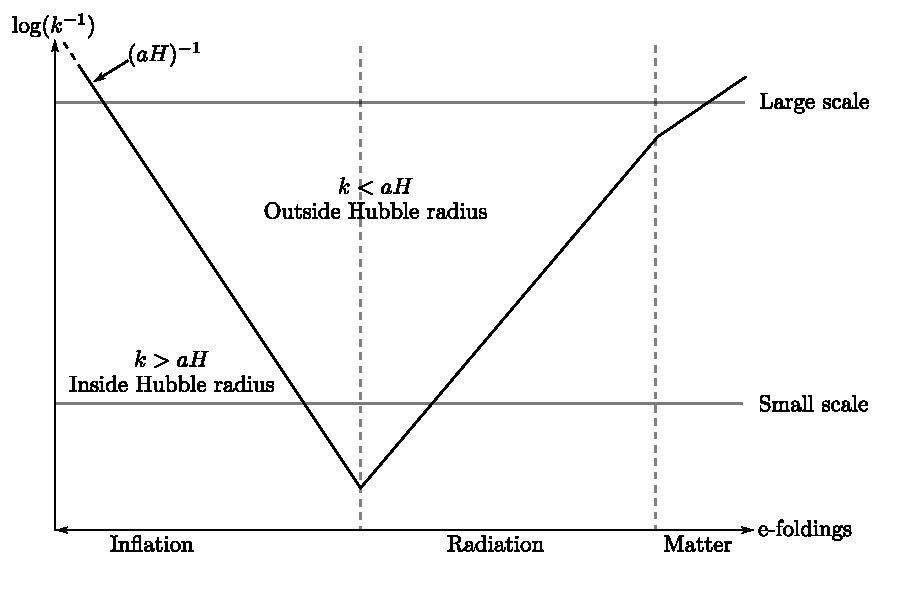
\includegraphics[width=\textwidth]{graphs/scales.pdf}
 \caption[Comoving Scales and the Hubble Radius]{Comoving scales that have recently
entered the horizon would
previously have been inside the horizon, if the inflationary period extended far
enough into the past.}
 \label{fig:comovingscales-intro}
\end{figure}
% 

Now consider the time derivative of $|\Omega -1|$ as defined in
\eq{eq:omegadefn-intro}:
% 
\begin{equation}
 \label{eq:omegaderiv-intro}
 \frac{\d}{\d t}\left(|\Omega -1 |\right) = 2\frac{\d}{\d t}
\left(\frac{1}{aH}\right)\,.
\end{equation}
% 
If the universe is not flat to begin with, a period of inflation of sufficient
duration will push it
towards $\Omega=1$, solving the flatness problem. Instead of an unstable point
in the parameter space, $\Omega=1$ is an attractor during the inflationary
phase. 
% 

To solve the horizon and flatness problems the duration of the inflationary era
must be
sufficiently long. Approximately $50$--$70$ e-foldings is considered standard
\cite{book:liddle}. Inflation
can last longer than this but only the last 50--70 e-foldings will be important
for the length scales of our observable universe. 


During inflation the universe is filled by material exhibiting negative isotropic
pressure.
Therefore, whatever drives inflation cannot be matter or radiation in their usual
forms. The simplest proposal is to fill the universe with a single scalar field
$\varphi$. The canonical action for this field is
\begin{equation}
\label{eq:phiaction-intro}
 \mathcal{L}_\mathrm{M} \equiv P(\varphi, X) = X -V(\varphi) \,,
\end{equation}
where $X=-\frac{1}{2}g_{\mu\nu}\partial^\mu\varphi \partial^\nu\varphi$ denotes
the kinetic energy of $\varphi$, $V(\vp)$ is the potential and $P(\varphi, X)$
is called the kinetic
function. In Section~\ref{sec:noncanoninfl} we will consider other
choices for $P$. 

The equation of motion for $\varphi$, for the canonical action $P=X-V$, is
% 
\begin{equation}
 \label{eq:phieom1-intro}
 \ddot{\vp} + 3H\dot{\vp} -\nabla^2 \vp + \frac{\delta V}{\delta \vp} = 0\,.
\end{equation}
% 
If we now restrict ourselves to considering the homogeneous part of the field,
$\vp=\vp(t)$, the $\nabla^2\vp$ term disappears and the functional derivative
of $V$ becomes a standard derivative $V_{,\vp}$. 
% A subscripted comma will
% denote partial differentiation, $V_{,\vp}=\partial V/\partial\vp$.
With these choices we have the following relations for the matter
energy-density and isotropic pressure:
% 
\begin{align}
\label{eq:EandP-intro}
 E &= \frac{1}{2}\dot{\varphi}^2 + V(\varphi) \,,\\
\label{eq:Pdefn-intro}
 P &= \frac{1}{2}\dot{\varphi}^2 - V(\varphi) \,.
\end{align}
% 
Under these conditions the kinetic function $P(\varphi, X)$ can be identified as
the isotropic pressure. The dynamics of the field are governed by the potential
$V(\varphi)$. Inflation requires $P<-E/3$, so from Eqs.~\eqref{eq:EandP-intro} and
\eqref{eq:Pdefn-intro} inflation
can also be thought of as a period when the potential energy dominates over
the kinetic energy. 


Inflation needs to last long enough to solve the problems described above. A generic
potential is not likely to satisfy these requirements without fine-tuning. One
approach is to enforce conditions on the potential under which the inflationary
period is necessarily long. 
% 
We have seen that for
inflation to occur the potential needs to dominate over the kinetic energy. From
\eq{eq:EandP-intro}, this occurs in the limit $P\rightarrow -E$ or equivalently
$\varepsilon_H \ll 1$. However, for this to remain the case for a sufficiently long
period the second derivative of $\vp$ must be small. If we define
another parameter 
% 
\begin{equation}
 \label{eq:etaHdefn-intro}
 \eta_H \equiv -\frac{\d \ln \dot{\vp}}{\d \ln a} =
-\frac{\ddot{\vp}}{H\dot{\vp}}
 =\varepsilon_H -\frac{\dot{\varepsilon_H}}{2H\varepsilon_H}\,,
\end{equation}
% 
then taking $|\eta_H|\ll 1$ ensures that $\dot{\vp}$ and $\varepsilon_H$
change slowly. This allows an inflationary phase of sufficient duration to occur.

The approximations $\varepsilon_H\ll 1$ and $|\eta|\ll 1$ are known as the
slow roll conditions because they force the inflaton field $\vp$ to roll down
the potential $V$ slowly. The parameters $\varepsilon_H$ and $\eta_H$ are the
slow roll parameters. Setting $\ddot{\vp}$ to be small is equivalent to
making the friction $H\dot{\vp}$ in \eq{eq:phieom1-intro} dominant. With
these approximations the
equations of motion for a slowly rolling field become
% 
\begin{align}
 \dot{\vp} &\simeq - \frac{V_{,\vp}}{3H}\,, \\
 H^2 &\simeq \frac{8\pi G}{3}V(\vp)\,.
\end{align}




% % % % % % % % % % % % % % % % % % % % % % % % % % % % % % % % 
% =========================================================== %
% % % % % % % % % % % % % % % % % % % % % % % % % % % % % % % % 
\section{Perturbations}
\label{sec:perts-intro}
% % % % % % % % % % % % % % % % % % % % % % % % % % % % % % % % 
% =========================================================== %
% % % % % % % % % % % % % % % % % % % % % % % % % % % % % % % % 

We considered a homogeneous scalar field in the analysis of
Section~\ref{sec:inflation-intro}. Such a field, however, will
lead only to a homogeneous universe later. How does the myriad structure
that we see around us form? From stars to galaxies to clusters, the
gravitational force has concentrated energy density over the history of the
universe, but some initial fluctuation must have been present to begin this
process. One of the main achievements of inflation is to provide a physical
origin for
such initial fluctuations. In Chapter~\ref{ch:perts} we will formally develop
cosmological perturbation theory up to second order. In this section we 
review first order perturbation theory and introduce the observable quantities
important for inflation.


Suppose that a full inhomogeneous scalar field
$\varphi$ is split into a homogeneous background field $\vp_0$, as described
above, and an inhomogeneous perturbation $\dvp{}(\eta,x^i)$ for $i=1,2,3$. For the
following
analysis to be applicable the perturbation must be much smaller than the background
field value. From the amplitude of perturbations in the CMB this approximation
can be seen to be valid \cite{Komatsu:2008hk}. 

If we suppose that $\epsilon$ is a small quantity then the split in $\vp$
can be written as \cite{Malik:2008im}
% 
\begin{equation}
\label{eq:pertsplit-intro}
\vp(\eta, x^i) = \vp_0(\eta) + \epsilon\dvp{}(\eta, x^i) \,.
\end{equation}
% 
 The perturbation $\dvp{}(\eta, x^i)$ can be further expanded in
powers of $\epsilon$.  We will follow the
custom of not explicitly writing $\epsilon$, instead relying on the order of
the perturbation, denoted by a subscript, to keep track.
If we expand in a Taylor series then up to second order (\ie including terms
up to $\epsilon^2$) we have:
% 
\begin{equation}
 \vp(\eta, x^i) = \vp_0(\eta) + \dvp1(\eta, x^i) + \frac{1}{2}\dvp2(\eta, x^i)
\,.
\end{equation}
% 
There is some freedom in how the split of the perturbations into different
orders is made. We will suppose that the first order perturbation $\dvp1$
contains only linear contributions and the higher order terms contain non-linear
terms. 


Instead of working in coordinate space, we can also consider
the perturbation in Fourier space using the definition
% 
\begin{equation}
\label{eq:fourierdefn-intro}
 \dvp{}(\eta, x^i) = \frac{1}{(2 \pi)^3} \int \d^3k \dvp{}(\kvi) \exp (i k_i
x^i)
\,,
\end{equation}
where $k^i$ are the components of the comoving wavenumber vector $\bf{k}$. The
amplitude of this
vector $k=|\bf{k}|$ identifies whether a particular mode is inside or outside
the comoving horizon. Wavemodes inside the comoving horizon are identified by
$k>aH$, while $k<aH$ for those outside the horizon. 


We must also consider perturbations in the metric tensor $g_{\mu\nu}$. If the
background metric is the FRW one described in Section~\ref{sec:frw-intro} then
the metric can be written with perturbations, up to first order, as follows:
% 
\begin{align}
 \label{eq:pertmetric-intro}
 g_{00} &= -a^2 (1 + 2\phi_1) \,, \nonumber\\
 g_{0i} &= a^2 B_{1i} \,, \nonumber\\
 g_{ij} &= a^2\left(\delta_{ij} + 2C_{ij} \right) \,.
\end{align}
% 
The $0$-$i$ and $i$-$j$ perturbations can be decomposed into scalar, vector and
tensor parts \cite{Malik:2008im}:
\begin{align}
\label{eq:svt-intro}
  B_{1i} &= B_{1,i} - S_{1i} \,, \nonumber\\
  C_{1ij} &= -\psi_1\delta_{ij} + E_{1,ij} + F_{1(i,j)} + \frac{1}{2}h_{1ij}\,.
\end{align}
% 
The vectors $S_{1i}$ and $F_{1i}$ are divergence free and the tensor part
$h_{1ij}$
is divergence free and traceless:
% 
\begin{equation}
 S^k_{1~,k} = 0\,, \quad F^k_{1~,k}=0\,; \qquad h^{ik}_{1~~,k} = 0\,,
  \quad h^k_{1~k}= 0\,.
\end{equation}
% 
In the previous equations $\phi$ is the lapse function, $\psi$ is the curvature
perturbation, $B_1$ and $E_1$ are the scalar part of the shear, $S_{1i}$, and
$F_{1i}$
are the vector parts of the shear, and $h_{1ij}$ is the tensor perturbation
describing gravitational waves.
% Scalar field inflation does not produce vector perturbations so we will not
% consider them  \cite{book:liddle}.


Splitting an inhomogeneous spacetime into background and perturbation is not a
covariant operation. This leads to an ambiguity in the choice of coordinates
which must be rectified by choosing a gauge. Gauge transformations relate
physical results in one gauge to those in another. To choose a gauge one must
specify how spacetime is foliated, \iec a slicing, and how coordinates in one
spatial hypersurface are related to those in another, \iec a threading
\cite{Malik:2008im}. We will
employ the uniform curvature gauge in which spatial hypersurfaces are flat. This
is also known as the flat gauge.

The gauge transformation vector at first order,  $\xi_1^\mu$, can be split into
scalar
and vector parts
% 
\begin{equation}
\label{eq:xidefn-intro}
 \xi_1^\mu = (\alpha_1, \beta_{1,}^{~i} + \gamma_1^i)\,,
\end{equation}
% 
where the vector part obeys $\gamma_{1~,k}^{~k}=0$. A scalar quantity such as
the inflaton perturbation will transform as \cite{Malik:2008im, Malik:2008yp}
% 
\begin{equation}
 \label{eq:dphitransform-intro}
 \wt{\dvp1} = \dvp1 + \vp_0' \alpha_1\,,
\end{equation}
where a tilde ($\wt{~}$) denotes a transformed quantity. For the metric
perturbations the
transformations for the scalars are
\begin{align}
 \label{transphi1}
\widetilde {\phi_1} &= \phi_1 +\H\alpha_1+\alpha_1'\,,\\
%
\label{transpsi1}
\widetilde \psi_1 &= \psi_1-\H\alpha_1 \,,\\
%
\label{transB1}
\widetilde B_1 &= B_1-\alpha_1+\beta_1'\,,\\
%
\label{transE1}
\widetilde E_1 &= E_1+\beta_1\,,
\end{align}
and for the vectors
\begin{align}
 \label{transS1}
\widetilde {S_{1}^{~i}} &= S_{1}^{~i}-\gamma_1'\,, \\
%
\label{transF1}
\widetilde {F_{1}^{~i}} &= F_{1}^{~i}+\gamma_1\,. 
\end{align}
% 
The tensor perturbation $h_{1ij}$ does not change under transformation at first
order, but does at subsequent orders.
The flat gauge, which we will use, is the one in which spatial hypersurfaces
are not perturbed by scalar or vector perturbations, so $\wt{\psi_1} = \wt{E_1}
=0$ and $\wt{F_{1i}} = \textbf{0}$.  This is equivalent to the transformation
% 
\begin{equation}
 \alpha_1 = \frac{\psi_1}{\H}\,,\quad \beta_1=E_1 \,, \quad \gamma^i_1 =
-F^i_1\,.
\end{equation}

A gauge invariant inflaton perturbation variable is the Sasaki-Mukhanov
variable \cite{Mukhanov:1990me, Mukhanov:1988jd,
Sasaki:1986hm}:
% 
\begin{equation}
\label{eq:flatdvp1-intro}
 \wt{\dvp1} \equiv \dvp1 + \vp_0'\frac{\psi_1}{\H}\,,
\end{equation}
% 
In the flat gauge this is just $\dvp1$. We will work in flat
gauge from now on and so will drop the tildes on quantities in that gauge.

Another very important gauge invariant quantity is the comoving curvature
perturbation $\R$. At first order in the flat gauge $\R$ is related to the
inflaton perturbation by \cite{Malik:2008im}
% 
\begin{equation}
\label{eq:flatRdefn-intro}
 \R = \frac{\H}{\vp_0'}\dvp1\,.
\end{equation}
% 
We are interested in the power spectrum of the curvature perturbation as this
is directly related to the temperature fluctuations that we can observe in the
CMB. 

The action \eqref{eq:phiaction-intro},
including perturbations of $\vp$ and $g_{\mu\nu}$ up to first order, is
varied to get the equation of motion of $\dvp1$. 
In the flat gauge the equation can be rewritten in terms of the inflaton field
values only by eliminating the metric perturbations using
\eq{eq:flatdvp1-intro}. 
% 
In Fourier space and in terms of the conformal time $\eta$, the closed form of
the first order perturbation equation of motion is \cite{Malik:2008im}
% 
\begin{multline}
\label{eq:fokg-intro}
\dvp1''(\kvi) + 2\H \dvp1'(\kvi) + k^2\dvp1(\kvi) \\
+ a^2 \left[\Upp +
\frac{8\pi G}{\H}\left(2\vp_{0}' \Uphi + (\vp_{0}')^2\frac{8\pi G
}{\H}\U\right)\right]\dvp1(\kvi) = 0 \,,
\end{multline}
% 
where $\U$ is the background value of the potential $V(\vp)$.
% 
Substituting $u=a\dvp1$ gives the Mukhanov equation \cite{Mukhanov:1990me}
% 
\begin{equation}
 \label{eq:ueq-intro}
 u''(\kvi) + \left[ k^2 -\frac{z''}{z}\right]u(\kvi) = 0\,,
\end{equation}
% 
where $z= a\vp_0'/\H$.

\subsection{Quantum Perturbations}
So far we have considered classical perturbations. However, the generation of
fluctuations is a quantum effect and we need to consider the
perturbations as quantum operators in some vacuum. 

In Minkowski space the quantisation of $u(\kvi)$ is straightforward.
The perturbation modes can be written in terms of quantum operators as
% 
\begin{equation}
 u(\kvi)\rightarrow\hat{u}(\kvi) = 
  w(\kvi) \hat{a}(\kvi) + w^\star(-\kvi)\hat{a}^\dagger(-\kvi) \,.
\end{equation}
%
The mode function $w(\kvi)$ obeys the same equation of motion as $u(\kvi)$:
% 
\begin{equation}
\label{eq:weqn-intro}
 w''(\kvi) + \left[ k^2 -\frac{z''}{a}\right]w(\kvi) = 0\,.
\end{equation}
% 
The operators $\hat{a}^\dagger$ and $\hat{a}$ are the usual creation and
annihilation operators. They act on quantum states by adding or
removing particles. The zero particle vacuum state, $|0\rangle$, is such that
% 
\begin{equation}
 \hat{a}^\dagger|0\rangle = |1\rangle\,,\quad \hat{a}|0\rangle = 0\,.
\end{equation}
% 
In Minkowski space these operators have the usual commutation relations
% 
\begin{equation}
 [\hat{a}(\kb), \hat{a}^\dagger(\kb')] = (2\pi)^3 \delta(\kb -\kb') \\
\end{equation}
and
\begin{equation}
[\hat{a}(\kb), \hat{a}(\kb')] = 0\,.
\end{equation}
% 
The $w$ modes are normalised by the condition \cite{Mukhanov:2005sc}
% 
\begin{equation}
\label{eq:quantcondition-intro}
 i(w^\star(\kvi)w'(\kvi) - {w^{\star}}'(\kvi)w(\kvi)) = 1\,.
\end{equation}


In the expanding FRW background the choice of vacuum is not straightforward.
Suppose one observer selects a zero particle state as the vacuum. Another
observer accelerating with respect to the first will see particles being
created in this ``vacuum'' state due to the Unruh effect
\cite{Kinney2009, Unruh1976a}. In selecting the vacuum we must choose one of the
many equivalent options.
To do this we consider the far past where $\eta\rightarrow -\infty$. The wavelengths of all the
modes are then much smaller than the Hubble radius and curvature scale. The modes are
therefore assumed to evolve in flat space. This suggests the Minkowski vacuum as the
most natural vacuum state to select and this choice of vacuum at
early times is known as the Bunch-Davies vacuum.
% 
In the limit $\eta\rightarrow -\infty$ (or equivalently $k/aH\rightarrow \infty$),
the mode equation
\eqref{eq:weqn-intro} becomes
% 
\begin{equation}
  w''(\kvi) + k^2 w(\kvi) = 0\,,
\end{equation}
% 
which has the plane wave solution
% 
\begin{equation}
\label{eq:subhsoln-intro}
 w(\kvi) = \frac{1}{\sqrt{2k}} e^{-ik\eta}\,.
\end{equation}
% 
This is the initial condition for modes which are well inside the horizon.

Now consider the de Sitter limit in which $\varepsilon_H\rightarrow 0$ and $H$
is constant. We have $z''/z = a''/a = 2/\eta^2$ so the mode equation is
% 
\begin{equation}
  w''(\kvi) + \left[ k^2 -\frac{2}{\eta^2} \right]w(\kvi) = 0\,.
\end{equation}
% 
A full general solution for $w$ is
% 
\begin{equation}
 w(\kvi) = A\frac{e^{-ik\eta}}{\sqrt{2k}}\left(1 -\frac{i}{k\eta}\right)
	  +B\frac{e^{+ik\eta}}{\sqrt{2k}}\left(1 +\frac{i}{k\eta}\right)\,.
\end{equation}
% 
Taking the condition \eqref{eq:quantcondition-intro} along with the solution
for subhorizon modes in \eq{eq:subhsoln-intro} we find that $A=1$ and $B=0$.
Thus the full solution in de Sitter space is \cite{book:liddle}
% 
\begin{equation}
\label{eq:wfinal-intro}
 w(\kvi) = \frac{e^{-ik\eta}}{\sqrt{2k}}\left(1 -\frac{i}{k\eta}\right)\,.
\end{equation}
% 
Inflation in spacetimes that are close to de Sitter will contain perturbations
with a spectrum defined by \eq{eq:wfinal-intro}. The slow roll approximation is
enough to ensure that inflation occurs in a quasi-de Sitter spacetime.
However, the initial conditions for Fourier modes in \eq{eq:subhsoln-intro}
apply to non slow roll models so long as they are applied well before horizon
crossing.


\subsection{Power Spectra and Spectral Indices}
The power spectrum of the inflaton perturbation $\dvp1 = u/a$ can now be
defined as
% 
\begin{equation}
  \langle \dvp1(\textbf{k}) \dvp1(\wt{\textbf{k}}) \rangle 
   \equiv (2\pi)^3 \delta(\textbf{k} + \wt{\textbf{k}}) P_{\dvp{}}^2 (k)
   = (2\pi)^3 \delta(\textbf{k} + \wt{\textbf{k}}) \frac{|w(\kb)|^2}{a^2}\,,
\end{equation}
% 
where $\langle \ldots \rangle$ denotes the ensemble average. 
If taken over a large enough volume, the ensemble average and spatial average
are equivalent \cite{book:lyth}.
The power spectrum
$P_{\dvp{}}^2$ depends only on the magnitude of the wavenumber
vector, $k=|\bf{k}|$, but has dimensions of $k^{-3}$. A dimensionless power
spectrum
can be defined as
% 
\begin{equation}
 \label{eq:curlPrdefn-intro}
 \mathcal{P}_{\dvp{}}^2= \Delta^2_{\dvp{}} \equiv \frac{k^3}{2\pi^2}
P_{\dvp{}}^2(k)\,.
\end{equation}
% 

In a similar way we can define the power spectrum of the comoving curvature
perturbation $\R = H\dvp1/\dot{\vp}_0$:
% 
\begin{equation}
 \label{eq:Prdefn-intro}
 \langle \R(\textbf{k}) \R(\wt{\textbf{k}}) \rangle 
   = (2\pi)^3 \delta(\textbf{k} + \wt{\textbf{k}}) P_\R^2 (k)\,,
\end{equation}
%
and the dimensionless power spectrum
% 
\begin{equation}
 \Pr= \Delta^2_{\dvp{}} \equiv \frac{k^3}{2\pi^2}
P_{\R}^2(k)\,.
\end{equation}

A slow roll inflation model in a quasi-de Sitter spacetime will have the
Fourier mode solution given in \eq{eq:wfinal-intro}. 
After horizon crossing, when $k\ll aH$, this gives $|w|^2 = 1/(2k^3 \eta^2)$ so 
% 
\begin{equation}
\label{eq:pphi-intro}
 \mathcal{P}_{\dvp{}}^2(k) = \left(\frac{H}{2\pi}\right)^2 \,,
\end{equation}
% 
for the scalar perturbation spectrum and
% 
\begin{equation}
 \Pr(k) = \left(\frac{H}{\dot{\vp_0}}\right)^2 \left(\frac{H}{2\pi}\right)^2\,,
\end{equation}
% 
for the comoving curvature perturbation spectrum. Models that are not
slowly rolling usually require their more complicated mode equations to be
numerically solved. 

We have discussed in depth the scalar perturbations but tensor perturbations
can also be produced. The tensor perturbation $h_{ij}$
has two polarisations, $h_s$ for $s=+, \times$. The amplitude of
each can be thought of as a separate scalar field. The analysis for each field
is similar to that above with the substitution $h_s= 2\dvp1/\Mpl$. After horizon
crossing in a quasi-de Sitter space the spectrum for each polarisation is
% 
\begin{equation}
 \mathcal{P}_h^2(k) = \frac{4}{\Mpl^2} \left(\frac{H}{2\pi}\right)^2\,,
\end{equation}
% 
and the overall tensor perturbation spectrum is
% 
\begin{equation}
 \label{eq:Ptdefn-intro}
\Pt(k) = \frac{2}{\Mpl^2} \frac{H^2}{\pi^2}\,.
\end{equation}
The ratio of the tensor to curvature perturbations (tensor-scalar ratio) $r$ is
defined as 
% 
\begin{equation}
 r = \frac{\Pt}{\Pr}\,,
\end{equation}
% 
where $r$ is usually quoted at a particular $k$ but could in principle depend
on $k$. The tensor-scalar ratio can also be written in terms of $\varepsilon_H$:
% 
\begin{equation}
\label{eq:rslowroll-intro}
 r = 16 \varepsilon_H\,.
\end{equation}
As $\varepsilon_H\ll1$ for slow roll models of inflation the amplitude of tensor
perturbations that these models produce is much smaller than the amplitude of
curvature perturbations. 


% Post spectra derivations
If the curvature perturbation power spectrum, $\Pr(k)$, is independent of
wavenumber $k$, it is said to be scale invariant. The spectral index $n_s$ is a
measure of the deviation from scale invariance:
% 
\begin{equation}
\label{eq:nsdefn-intro}
 n_s -1 = \frac{\d \ln (\Pr(k))}{\d \ln k}\,,
\end{equation}
% 
where $n_s=1$ denotes a scale invariant spectrum. The spectral index of
the tensor power spectrum can be similarly defined:
% 
\begin{equation}
\label{eq:ntdefn-intro}
 n_T = \frac{\d \ln(\Pt(k))}{\d \ln k}\,,
\end{equation}
although this definition means that the spectrum is scale invariant if
$n_T=0$.
The spectral indices and indeed the spectra themselves are usually calculated
at an arbitrary pivot scale. The WMAP results for $\Pr$ and $\Pt$ outlined in
Section~\ref{sec:obs-intro} are quoted at the scale $k=0.002\Mpc^{-1}$.


If there is a non-trivial dependence of $\Pr$ or $\Pt$ on $k$ then higher order
derivatives can be taken to give the running of the quantities. The runnings
of the spectral indices are
% 
\begin{equation}
\label{eq:runningsdefn-intro}
 \alpha_s = \frac{\d \ln n_s}{\d \ln k}\,, \quad 
  \alpha_T = \frac{\d \ln n_T}{\d \ln k}\,.
\end{equation}

In the slow roll approximation $n_s$ and $n_T$ can be written in terms of the slow
roll parameters $\epsilon_H$ and $\eta_H$, evaluated at $k=aH$ using $\d \ln(aH)
\simeq H\d t$:
% 
\begin{align}
 n_s -1 &= -4\epsilon_H + 2\eta_H\,, \\
 n_T &= -2\epsilon_H \label{eq:ntslowroll-intro}\,.
\end{align}
% 
Combining \eq{eq:ntslowroll-intro} and \eq{eq:rslowroll-intro} gives a
powerful consistency condition for slow roll inflation:
% 
\begin{equation}
 \label{eq:consistency-intro}
 r = -8 n_T \,.
\end{equation}
% 
For the slow roll approximation to be valid for single field canonical inflation
models, \eq{eq:consistency-intro} must hold. Current observations are not accurate
enough to test this condition but it is hoped that this will be possible in the
future.


% % % % % % % % % % % % % % % % % % % % % % % % % % % % % % % % 
% =========================================================== %
% % % % % % % % % % % % % % % % % % % % % % % % % % % % % % % % 
\section{Current Observations}
\label{sec:obs-intro}
% % % % % % % % % % % % % % % % % % % % % % % % % % % % % % % % 
% =========================================================== %
% % % % % % % % % % % % % % % % % % % % % % % % % % % % % % % % 
There have been rapid improvements in the quantity and quality of cosmological data
sources in the last twenty years. From the launch of the COBE satellite in
1989 \cite{Bennett1994, Bennett1996c}, through the currently
ongoing WMAP mission \cite{spergel, Komatsu:2008hk}, to the recent launch of the
Planck satellite \cite{planck}, space based observations have been at the
forefront of the effort to collect data. Complementing these have been ground
and balloon based missions including CBI
\cite{Mason2003b, Sievers2003, Sievers2007}, VSA \cite{Dickinson2004}, ACBAR
\cite{Kuo2004, Kuo2007} and BOOMERANG \cite{Ruhl2003, Montroy2006,
Piacentini2006}.

Major recent data releases have provided significant confirmation of the FRW
model of the universe. The Hubble parameter today has been measured as $H_0 =
72\pm8\,\mathrm{km}/\mathrm{s}/\Mpc$ by the Hubble Key Project
\cite{Freedman2001}. The WMAP 5-Year data release (WMAP5) \cite{Komatsu:2008hk}
quotes their results combined with
data from Baryon
Acoustic Oscillations in galaxy distributions (BAO) \cite{Percival2007}
and supernova surveys (SN) by the Hubble Space Telescope and others \cite{Riess2004,
Riess2007, Astier2006, Wood-Vasey2007}. 
% the SuperNova Legacy Survey \cite{Astier2006}, and ESSENCE
% \cite{Wood-Vasey2007}. 
This combined data constrains the
universe to within two percent of the flat $\Omega =1, K=0$ case outlined in
Section~\ref{sec:frw-intro}. 

The amplitude of the scalar curvature perturbations $\Pr$ was first measured
accurately by the COBE satellite \cite{Bennett1994, Bennett1996c}. The WMAP5
normalisation is taken at a different scale to the COBE result, measuring
% 
\begin{equation}
 \label{eq:wmapnorm-intro}
 \Pr(\kwmap) = 2.457 \e{-9}\,,
\end{equation}
% 
where the pivot scale $\kwmap = 0.002\Mpc^{-1} \simeq 5.25\e{-60}\Mpl$. The
spectral index of scalar perturbations for models with tensor-scalar ratio
$r\ne0$ is given by the combined WMAP5+BAO+SN measurement as
% 
\begin{equation}
 \label{eq:wmapns-intro}
 n_s = 0.968 \pm 0.015\,,
\end{equation}
% 
and $r$ in this case is bounded by
% 
\begin{equation}
\label{eq:rbound-intro}
 r < 0.54\,,
\end{equation}
at the 95\% confidence level.






% % % % % % % % % % % % % % % % % % % % % % % % % % % % % % % % 
% =========================================================== %
% % % % % % % % % % % % % % % % % % % % % % % % % % % % % % % % 
\section{Non-Canonical Inflation} 
\label{sec:noncanoninfl}
% % % % % % % % % % % % % % % % % % % % % % % % % % % % % % % % 
% =========================================================== %
% % % % % % % % % % % % % % % % % % % % % % % % % % % % % % % % 

In the previous section we considered the dynamics of a scalar field with a
canonical action $P(\vp, X) = X - V(\vp)$, where $X \equiv -\frac{1}{2}g^{\mu
\nu}\nabla_\mu \varphi \nabla_\nu \varphi$ is the kinetic energy. 
In this
section we will generalise
that analysis to include non-canonical actions. Non-canonical scalar
field actions appear frequently in string theory derived inflationary models.
In Chapters~\ref{ch:dbi-intro}, \ref{ch:dbi} and \ref{ch:multibrane}
there are explicit examples of non-canonical scenarios.

We will consider an action of the same form as before
% 
\begin{equation}
\label{eq:DBIaction-dbiintro2}
S=\int  \d^4x \sqrt{|g|} \left[ \frac{\Mpl^2}{2} R 
+ P (\varphi , X) \right] \,,
\end{equation}
% 
with minimal coupling to the gravitational sector. Varying this action gives the
stress-energy tensor in
\eq{eq:fluidstress-intro} where $u_\mu = \partial_\mu\vp/\sqrt{2X}$. 
% Insert energy momentum tensor.
The energy density $E$ is defined as
\begin{equation}
 E = 2X\PX - P\,,
\end{equation}
% 
and for a homogeneous scalar field the kinetic term $P(\vp, X)$ is the
isotropic pressure. 
It proves convenient to define two parameters in terms of the 
kinetic function $P$ and its derivatives \cite{lidser1,lidser3}: 
% 
\begin{align}
\label{eq:defcs-dbiintro}
 c_s^2 &\equiv \frac{\PX}{E_{,X}} =  \frac{\PX}{\PX + 2X P_{,XX}} \,,
\\
\label{eq:deflambda-dbiintro}
\Lambda &\equiv  \frac{X^2 P_{,XX} +
\frac{2}{3}X^3 P_{,XXX}}{X P_{,X} +
2X^2 P_{,XX}}\,.
\end{align}
% 
The first parameter, $c_s$, is called the sound speed of the fluctuations
in the inflaton field. This can be significantly less than unity for non-canonical
actions, 
in contrast to slow roll inflation driven by a canonical 
field such that $c_s = P_{,X} =1$.
% 
Christopherson \& Malik showed in \Rref{Christopherson:2008ry} that $c_s$
is in fact the phase speed of the fluctuations and not the sound speed
which is defined as $\dot{P}/\dot{E}$. However, in common with the rest of the
literature, we will continue to use $c_s$ as defined in \eq{eq:defcs-dbiintro}. 

The generation of quantum perturbations in the non-canonical case is similar to
the canonical one, but now includes contributions from $c_s$. Letting
$u=a\dvp1$, the Mukhanov equation for the
Fourier modes, \eq{eq:ueq-intro}, becomes
\cite{gm}:
% 
\begin{equation}
 u''(\kvi) + \left[c_s^2 k^2 - \frac{z''}{z}\right] u(\kvi) = 0\,,
\end{equation}
% 
where $z$ has been redefined as
% 
\begin{equation}
 z = \frac{a\sqrt{E+P}}{c_s H} = \frac{a\sqrt{2X\PX}}{c_s H} \,.
\end{equation}
% 
We quantise the $u$ modes using the Bunch-Davies vacuum as above and work with the
amplitude $w(\kvi)$. Instead of considering whether modes are
inside the comoving horizon, it is now important to distinguish between modes
inside and outside the sound horizon, defined by $kc_s = aH$. Far inside the sound
horizon, where $kc_s \gg aH$, the mode solution takes a similar asymptotic form to
\eq{eq:subhsoln-intro}:
% 
\begin{equation}
 w(\kvi) = \frac{1}{\sqrt{2kc_s}} e^{-ikc_s \eta}\,.
\end{equation}


Following the same analysis as above, the amplitude of the curvature 
perturbations 
generated during inflation can be found and is given by
\cite{gm}
% 
\begin{equation} 
\label{eq:Ps-dbiintro}
 \Pr = \frac{H^4}{8\pi^2 X}\frac{1}{c_s \PX} \,.
\end{equation}
% 
This expression is only valid after exit from the sound horizon. In contrast
the tensor perturbations are not affected by the change in the action. The
expression for the power spectrum $\Pt$ in \eq{eq:Ptdefn-intro} is still valid.
This should be evaluated after the modes have exited the normal horizon,
\iec when $k < aH$. 
The consistency relation \eqref{eq:consistency-intro} is now defined as
\cite{gm} 
% 
\begin{equation}
\label{eq:rdefn-dbiintro}
  r = 16c_s \varepsilon_H = -8c_s n_T \,.
\end{equation}
% 
Hence, a sound speed different to unity leads to a violation of the 
standard inflationary consistency equation, which might be 
detectable in the foreseeable future \cite{lidser1,lidser2}. 




% % % % % % % % % % % % % % % % % % % % % % % % % % % % % % % % 
% =========================================================== %
% % % % % % % % % % % % % % % % % % % % % % % % % % % % % % % % 
\section{Non-Gaussianity}
\label{sec:fnl-intro}
% % % % % % % % % % % % % % % % % % % % % % % % % % % % % % % % 
% =========================================================== %
% % % % % % % % % % % % % % % % % % % % % % % % % % % % % % % % 
The initial fluctuations described above have Gaussian statistics, with no
correlations between modes
on different scales. All the information about the perturbations can be obtained from the
two-point function or power spectrum as defined in \eq{eq:Prdefn-intro}. For a
Gaussian random 
field all higher point functions are either zero or combinations of the two-point function. In
particular the three-point function of $\R$, $\langle
\R(x_1)\R(x_2)\R(x_3)\rangle$, will be zero for purely Gaussian $\R$. We can
write the Fourier
transform of the three point function in terms of the bispectrum $B$
\cite{Bartolo:2004if}:
% 
\begin{equation}
 \langle \R(\kb_1)\R(\kb_2)\R(\kb_2)\rangle = (2\pi)^3 \delta^3(\kb_1 + \kb_2 + \kb_3) B(k_1, k_2,
k_3)\,,
\end{equation}
% 
where translation invariance imposes the conservation of the $\kb$ vectors and
the bispectrum
depends only on the magnitude of each wavenumber. Any deviation from Gaussianity
will result in a
non-zero bispectrum value. 
Because of the delta-function, the wavevectors form triangles in Fourier
space and $B$ is a function of only two variables. The bispectrum generated by
inflationary models
takes two main triangular shapes, squeezed and equilateral \cite{Babich:2004gb}.
 
The first parametrisation of non-Gaussianity was defined in
real space in terms of the Gaussian part of the perturbation. As the
non-linearity is localised in real space the parameter is
known as the local non-Gaussianity $\fnlloc$: 
% 
\begin{equation} 
\label{eq:fnllocdefn-intro}
{\cal{R}} = {\cal{R}}_G + \frac{3}{5} \fnlloc  (
{\cal{R}}_G^2 -\langle {\cal{R}}_G^2 \rangle )\,.
\end{equation}
Here the 
quadratic component represents a convolution and 
$\R_G$ denotes the Gaussian contribution
\cite{Maldacena:2002vr}\footnotemark.
\footnotetext{We use the WMAP sign convention for $\fnl$ throughout. 
This is the opposite of the Maldacena convention:
$\fnl^\mathrm{WMAP}=-\fnl^\mathrm{Maldacena}$.}
The local non-Gaussian parameter $\fnlloc$ can be related to the bispectrum by:
\begin{equation}
 B(k_1, k_2, k_3) = \frac{6}{5}\fnlloc \left[P_\R^2(k_1)P_\R^2(k_2) +
P_\R^2(k_2)P_\R^2(k_3) + P_\R^2(k_3)P_\R^2(k_1)\right]\,.
\end{equation}
% 
If $P_\R^2(k)$ is approximately scale invariant, $P_\R^2(k) = c k^{-3}$, then
the bispectrum becomes \cite{Baumann2009}
% 
\begin{equation}
 B(k_1, k_2, k_3) = \frac{6}{5}\fnlloc c^2\left[\frac{1}{k_1^3 k_2^3} +
\frac{1}{k_2^3 k_3^3} + \frac{1}{k_3^3 k_1^3}\right]\,.
\end{equation}
% 
This expression is maximised if one of the $k_i$ is much smaller than the other two.
Momentum
conservation then requires that they are approximately equal. This
configuration is a squeezed triangle in momentum space where, for example, $k_3 \ll
k_1,k_2$. In
single field inflation $\fnlloc$ is proportional to the slow roll parameters
and therefore expected to be small. Non-linear contributions from the coupling
of the gravitational potential to the curvature perturbation are expected to
produce $\fnlloc$ of order one which would be much larger than the
$O(\varepsilon_H)$ contributions from single field, slow roll inflation
\cite{Bartolo:2004if, Komatsu:2008hk}. Any detection of $\fnlloc$ at greater
than $O(1)$ would present a challenge to such single field slow roll models. 
The current bounds on the non-Gaussianity parameter are not strong but have
been steadily tightening. The WMAP5 bound on the local form of $\fnl$ is
% 
\begin{equation}
\label{eq:fnlloc-wmap5-intro}
 -9<\fnlloc<111\,.
\end{equation}
% 
This observational limit still includes $\fnlloc=0$ at the 95\% confidence level.


The other important case is   
where the three momenta have equal magnitude, which corresponds to the
equilateral triangle limit. Non-Gaussianity of this shape is chiefly produced
by models with non-canonical kinetic terms as defined in
Section~\ref{sec:noncanoninfl}. The equilateral non-Gaussianity parameter
$\fnleq$ can be evaluated in terms of the sound speed $c_s$ and the
$\Lambda$ parameter defined in \eq{eq:deflambda-dbiintro}.
The leading-order contribution to the
non-linearity 
parameter is given by \cite{chenetal,lidser3}
% 
\begin{equation} 
\label{eq:fnldefn-dbiintro}
 \fnl = -\frac{35}{108}\left(\frac{1}{c_s^2} -1 \right) +
\frac{5}{81}\left( \frac{1}{c_s^2} -1 -2\Lambda \right) \,.
\end{equation}
%  
Data from WMAP3 imposed the bound $|\fnl| < 300$ on this parameter
\cite{spergel}. The more recent WMAP5 data set
improves on this bound somewhat \cite{Komatsu:2008hk}, and
also indicates that it is distinctly asymmetric. At the $95 \%$ confidence
level, the current bound on the 
equilateral triangle is 
% 
\begin{equation}
\label{eq:fnleq-wmap5-intro}
 -151<\fnleq<253\,.
\end{equation}
% 
% Other groups have re-examined the WMAP data
% and included previously absent parameter regions. 


% % % % % % % % % % % % % % % % % % % % % % % % % % % % % % % % 
% =========================================================== %
% % % % % % % % % % % % % % % % % % % % % % % % % % % % % % % % 
\section{Discussion}
\label{sec:disc-intro}
% % % % % % % % % % % % % % % % % % % % % % % % % % % % % % % % 
% =========================================================== %
% % % % % % % % % % % % % % % % % % % % % % % % % % % % % % % % 

In this chapter the physics of the FRW universe has been described. Inflation has been introduced
to solve problems with the standard Big Bang scenario. To solve these problems the
inflationary
period must be of sufficient duration. This can be ensured by using models which comply with
certain slow roll conditions. 

To explain inhomogeneities in the early universe, cosmological perturbation theory
was presented up
to first order. The power spectrum of scalar perturbations, $\Pr$, the spectral index of this
spectrum, $n_s$, and the ratio of tensor-scalar perturbations, $r$, are the main
observable
quantities against which models can be tested. Slow roll models must also satisfy a
consistency
relation between the tilt of the tensor spectrum and $r$. Current observations favour an almost
scale invariant red spectrum ($n_s<1$) with a low level of tensor signal. The accuracy of the
current data is not yet good enough to meaningfully evaluate the slow roll consistency relation. 

As well as the standard models, one can also construct inflationary models in which the action
takes a non-canonical form. In these models the sound speed of scalar fluctuations, $c_s$, plays a
pivotal role. The predictions for scalar perturbations are altered by a factor of $c_s$, as is the
slow roll consistency relation. Non-canonical models also often exhibit strong non-linear effects
which can be parametrised using the non-Gaussianity parameter $\fnl$. Canonical single field slow
roll models do not predict large amounts of non-Gaussianity. 

This chapter laid the foundations for the two main parts of this work in which first
analytic
and then numerical techniques are used to constrain inflationary models. In the next chapter the
DBI brane inflation scenario is presented. 


%%%%%%%%%%%%%%%%
%%%%%%%%%%%%%%%%
\part{DBI inflation}
\label{part:dbi}
% % % % % % % % % % % % % % % % % % % % % % 
% dbi.tex - Ian Huston
% $Id: dbi.tex,v 1.69 2009/12/07 16:43:29 ith Exp $
% % % % % % % % % % % % % % % % % % % % % 
% Redefine CVSRevision for this section
\renewcommand{\CVSrevision}{\version$Id: dbi.tex,v 1.69 2009/12/07 16:43:29 ith Exp $}

% % % % % % % % % % % % % % % % % % % % % % % % % % % % % % % % 
% =========================================================== %
% % % % % % % % % % % % % % % % % % % % % % % % % % % % % % % % 
\chapter{Observational Bounds on DBI Inflation}
\label{ch:dbi}
% % % % % % % % % % % % % % % % % % % % % % % % % % % % % % % % 
% =========================================================== %
% % % % % % % % % % % % % % % % % % % % % % % % % % % % % % % % 
% 
% 
% 
% % % % % % % % % % % % % % % % % % % % % % % % % % % % % % % % 
% =========================================================== %
% % % % % % % % % % % % % % % % % % % % % % % % % % % % % % % % 
\section{Introduction}
\label{sec:intro-dbi}
% % % % % % % % % % % % % % % % % % % % % % % % % % % % % % % % 
% =========================================================== %
% % % % % % % % % % % % % % % % % % % % % % % % % % % % % % % % 

In this chapter two bounds on the amplitude of primordial gravitational waves will be derived, which
severely challenge the standard
DBI inflationary scenario. By considering the field range of observable
inflation inside a warped throat, the tensor-scalar ratio $r$ will be
constrained to be less than $10^{-7}$. In contrast a lower bound of $r\gtrsim
0.005$ will be derived when the power spectrum of scalar perturbations has a red
spectral index. These clearly incompatible bounds can be relaxed by using a more
general form of the DBI action.

% 
The gravitational wave background generated in DBI 
inflation was initially investigated by Baumann \& McAllister (BM) 
\cite{bmpaper}. By exploiting a relationship due originally 
to Lyth \cite{lyth}, these authors derived a field-theoretic upper limit 
to the tensor amplitude and concluded that 
rather stringent conditions would need to be satisfied for these 
perturbations to be detectable.      
Moreover, the special case of 
DBI inflation driven by a quadratic potential is incompatible with the WMAP3 
data when this constraint is imposed \cite{bean}.  


Our aim in this chapter is to derive observational constraints on DBI inflation
that are 
insensitive to the details of the throat geometry and the inflaton potential. 
In general, there are two realisations of the scenario, 
which are referred to as the ultra-violet (UV) and infra-red (IR) 
versions. These are characterised respectively by whether the brane is 
moving towards or away from the tip of the throat. 
We focus initially on the UV scenario 
and derive an upper bound on 
the gravitational wave amplitude in terms of observable 
parameters. This limit arises by considering 
the variation of the inflaton field during the era when 
observable scales cross the Hubble radius, and 
we find in general that the tensor-scalar ratio must satisfy 
$r \lesssim 10^{-7}$. This 
is below the projected sensitivity of future CMB
polarisation 
experiments \cite{Baumann:2008aq,vpj}. 

On the other hand, the WMAP5 data 
favours a red perturbation spectrum, with 
$n_s<1$, when  
the scalar spectral index is effectively constant \cite{Komatsu:2008hk}. 
For models which generate such a spectrum, 
we identify a corresponding lower limit on the 
tensor modes such that $r \gtrsim 0.1 (1-n_s)$. 
This is incompatible with the upper bound 
on $r$ when $1-n_s \simeq 0.03$, as inferred
by the observations. 

Therefore a reconciliation between theory and observation 
requires either a relaxation of the upper limit on $r$ or a blue 
spectral index $(n_s >1)$. The DBI scenario would need 
to be generalised in a suitable way for the upper bound on $r$
to be weakened. Necessary conditions are identified that a 
generalised action must satisfy for the BM constraint and our newly derived
bound to be relaxed. 
Such conditions are shown in Chapter~\ref{ch:multibrane} to be
realised in a recently proposed IR version of DBI inflation driven
by multiple coincident branes \cite{thomasward}. 

% 
% 
% % % % % % % % % % % % % % % % % % % % % % % % % % % % % % % % 
% =========================================================== %
% % % % % % % % % % % % % % % % % % % % % % % % % % % % % % % % 
\section{An Upper Bound on the Primordial Gravitational Waves}
% 
\label{sec:upper-dbi}
% % % % % % % % % % % % % % % % % % % % % % % % % % % % % % % % 
% =========================================================== %
% % % % % % % % % % % % % % % % % % % % % % % % % % % % % % % % 
%

In \Rref{bmpaper} Baumann \& McAllister
derived a field-theoretic upper bound on the tensor-scalar ratio. They achieved
this by noting that the four-dimensional Planck mass is related 
to the volume of the compactified CY manifold, $V_6$, such that 
$\Mpl^2=V_6 \kappa_{10}^{-2}$, where $\kappa_{10}^2 \equiv 
\frac{1}{2} (2\pi )^7 \gs^2 \ms^{-8} = \pi /T_3^{2}$ for a 
${\rm D3}$-brane\footnote{We parametrise the Planck scale 
in terms of the ${\rm D3}$-brane tension out of convenience, 
and note that there is no physical relationship between the two.}.
In general, the compactified volume 
is comprised of bulk and throat contributions, 
$V_6 = V_{6\,{\rm bulk}}+V_{6\,{\rm throat}}$. The latter is 
given by
% 
\begin{equation}
\label{eq:throatvolume}
V_{6\,\mathrm{throat}} = \mathrm{Vol}(X_5)  
\int_0^{\rho_{UV}} \d\rho \frac{\rho^5}{h^4(\rho )} \,,
\end{equation}
% 
where $\rho_{UV}$ denotes the radial coordinate at 
the edge of the throat (defined as the region 
where $h (\rho_{UV})$ is of order unity). The geometry of the throat is shown
in Figure~\ref{fig:throat-geom}.

% 
\begin{figure}[htbp]
 \centering
 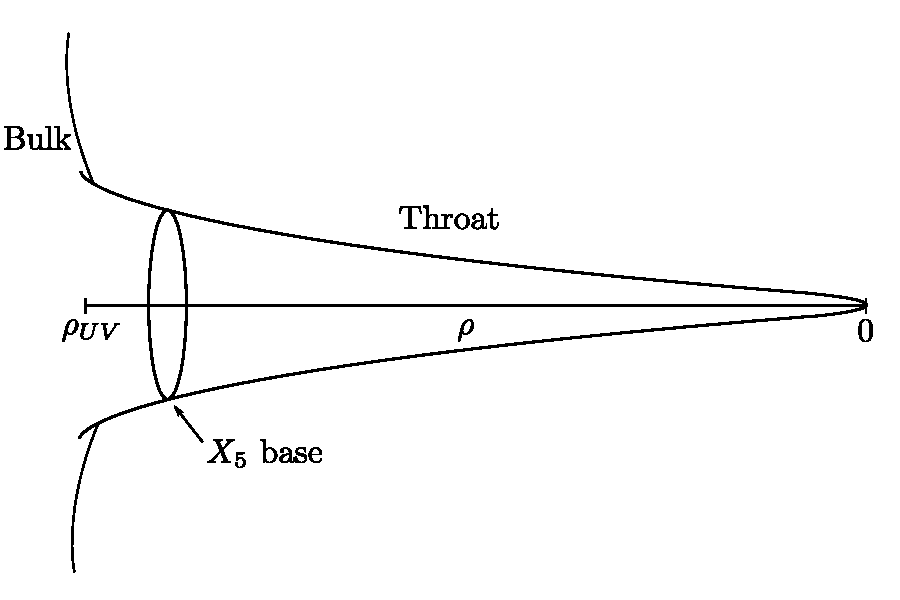
\includegraphics[width=\textwidth]{./dbi/graphs/throat-geom.pdf}
 % throat-geom.pdf: 432x288 pixel, 72dpi, 15.24x10.16 cm, bb=0 0 432 288
 \caption[Warped Throat Geometry]{Geometry of the warped throat. The radial
coordinate $\rho$ is measured from the tip of the throat to $\rho_{UV}$ at the join
with the bulk manifold.}
 \label{fig:throat-geom}
\end{figure}

% 

If one assumes that the bulk volume is 
non-negligible relative to 
that of the throat ($V_{6\,\mathrm{throat}} < V_{6}$), 
it follows that $\Mpl^2> V_{6\,\mathrm{throat}}\kappa_{10}^{-2}$. 
For a warped $AdS_5 \times X_5$ geometry, this leads to an 
upper limit on the total variation of the inflaton field in 
the throat region in terms of the D3 charge:
% 
\begin{equation}
\label{eq:BMbound-dbi}
\frac{\varphi_{UV}}{\Mpl}   < \frac{2}{\sqrt{N}} \,.
\end{equation}
% 


Condition (\ref{eq:BMbound-dbi}) may be converted into a 
corresponding limit on the tensor-scalar ratio by noting from 
the definition (\ref{eq:epsdefn-dbiintro})
that $\dot{\varphi}^2 /\Mpl^2 = 2\varepsilon_H H^2/P_{,X}$.
This implies that the variation of the inflaton field 
is given by the Lyth bound \eqref{eq:genlyth-dbiintro} 
\cite{lyth,bmpaper}:
% 
\begin{equation}
\label{eq:rtheory}
\frac{1}{\Mpl^2} \left( \frac{\d\varphi}{\d \N} \right)^2 =
\frac{r}{8} \,,
\end{equation}
% 
where $\N$ is the number of e-foldings as defined in \eq{eq:nefolddefn-intro}. 
Since $\vp_*$, the field value during observable inflation,  is
less than $\varphi_{UV}$,
this results in an upper bound on the observable tensor-scalar ratio
\cite{bmpaper}: 
% 
\begin{equation}
\label{eq:BMboundr}
r_*  < \frac{32}{N (\Neff)^2} \,.
\end{equation}
% 
The effective number of e-foldings, $\Neff$, defined in
\eq{eq:Neff-dbiintro}, 
is a model-dependent parameter that quantifies 
how $r$ varies during the final stages of inflation. Since $\cs\PX = 1$ in the
standard DBI model, 
it follows that $\Neff = \N_\mathrm{end}$ if $r$ is constant during inflation,
where $\N_\mathrm{end}$ is the total number of e-foldings
from the epoch of observable inflation until inflation ends.


Typically, one expects $30 \lesssim {\Neff} \lesssim 60$, 
although smaller values may be possible if the slow roll conditions are 
violated after observable scales have crossed the horizon. 
Furthermore, $N \gg 1$ is necessary 
for backreaction effects to be negligible \cite{bmpaper}. 
Hence, the constraint \eqref{eq:BMboundr} 
imposes a strong restriction on DBI inflationary models. 
On the other hand, the numerical value 
of $\Neff$ is uncertain.  
Our aim here is to focus on the range of values covered by the 
inflaton field during the observable stages of inflation. 
This will result in a constraint on the tensor modes that 
can be expressed in terms of observable parameters.  


To proceed, we denote the change in the value of the inflaton field over 
observable scales by 
$\Delta  \varphi _{*} = \sqrt{T_3} \Delta \rho_{*}$. 
Since the brane moves towards the tip of the throat in 
UV DBI inflation, it follows that $\rho_{*} > \rho_{end} >0$, which 
implies that  
% 
\begin{equation}
\label{eq:importantbound}
\rho_{*} > |\Delta \rho _{*}| \,.
\end{equation}
% 
This change in the inflaton value will correspond 
to a fraction of the throat volume, 
$| \Delta V _{6\,*}|  < {V_{6\,\mathrm{throat}}} \lesssim {V_6} $,
where equality in the second limit arises if
the bulk volume is negligible. Hence, 
$| \Delta \varphi_* |$ is bounded such that  
% 
\begin{equation}
\label{eq:halfwayconstraint}
\left( \frac{\Delta \varphi}{\Mpl} \right)^2_{*} < 
\frac{T_3 \kappa_{10}^2 (\Delta \rho_{*})^2}{|\Delta V_{6\,*}|} \,.
\end{equation}
%  


The observations of the CMB 
that directly constrain the primordial tensor perturbations only 
cover multipole values in the range $2 \le l \lesssim 100$. 
This is equivalent to ${\Delta \N_{*}} \simeq {4}$ 
e-foldings of inflationary expansion and, in general,   
corresponds to a narrow range of inflaton values. 
To a first approximation, therefore, the fraction of the throat volume 
(\ref{eq:throatvolume}) that is accessible to cosmological 
observation can be estimated to be 
% 
\begin{equation}
\label{eq:trapezium}
| \Delta V_{6\,*} | \simeq \mathrm{Vol}(X_5) 
\frac{|\Delta \rho_*| \rho^5_{*}}{h^{4}_{*}} \,.
\end{equation}
% 
Combining the inequality (\ref{eq:importantbound}) with \eq{eq:trapezium} 
then implies that 
% 
\begin{equation}
\label{eq:trapeziumlimit}
|\Delta V _{6\,*}| > \mathrm{Vol}(X_5) 
\frac{(\Delta \rho_* )^6}{h^{4}_*}  \,.
\end{equation}
% 
Substituting the condition \eqref{eq:trapeziumlimit} into the bound
\eqref{eq:halfwayconstraint} gives
\begin{equation}
\label{eq:hbound6}
\left( \frac{\Delta \varphi}{\Mpl} \right)_*^6 < \frac{\pi T_3}{\Vol} 
\left( \frac{h_*}{\Mpl} \right)^4 \,,
\end{equation}   
and using $T(\vp) = T_3 h^4$ and 
\eq{eq:obswarp-dbiintro} yields the upper limit
% 
\begin{equation}
\label{eq:boundpower6}
\left( \frac{\Delta \varphi}{\Mpl} \right)^6_{*} 
< \frac{\pi^3}{16\mathrm{Vol}(X_5)} r^2 \Pr 
\left( 1- \frac{1}{3\fnleq} \right)  \,.
\end{equation}
% 
Hence, employing the Lyth bound \eqref{eq:rtheory} in the form
$(\Delta \varphi_* / \Mpl )^2 \simeq 
r (\Delta \N_*)^2 /8$  
results in a very general upper limit on the tensor-scalar ratio: 
% 
\begin{equation}
\label{eq:generalbound}
r_{*} < \frac{32 \pi^3}{(\Delta \N_*)^6 \mathrm{Vol}(X_5)} 
\Pr \left( 1- \frac{1}{3\fnleq} \right) \,.
\end{equation}
% 


Condition (\ref{eq:generalbound}) is 
only weakly dependent on the level of non-Gaussianity 
when $-\fnleq > 5$ and we may therefore neglect the 
factor involving this parameter. 
Substituting the WMAP5 normalisation 
$\Pr \simeq 2.5 \times 10^{-9}$ then implies that
%  
\begin{equation}
\label{eq:upperbound}
r_{*} < \frac{2.5\times 10^{-6}}{( \Delta \N_*)^6 \mathrm{Vol}(X_5)} \,.
\end{equation}
% 
Furthermore, the most optimistic 
estimate for the minimum number of e-foldings that could be 
probed by observation is $\Delta \N_{*} \simeq 1$, whereas
a generic compactification arises when 
the volume of the Einstein five-manifold is $\mathrm{Vol}(X_5) 
\simeq {\cal{O}} (\pi^3)$ \cite{ks}. This yields a model-independent 
upper bound on the tensor-scalar ratio for standard UV DBI inflation:
%    
\begin{equation}
\label{eq:standardbound}
r_* < 10^{-7} \,.
\end{equation}
% 
The bound \eqref{eq:standardbound} is the main result of this section.
This value of $r$ is significantly below the sensitivity 
of future CMB polarisation experiments, which will measure 
${r} \gtrsim 10^{-4}$ \cite{Baumann:2008aq,vpj}. 
If CMB  
observations are able to span the full range of e-foldings such that
$\Delta \N_* \simeq 4$, this constraint is strengthened to 
${r_*} \lesssim {2 \times 10^{-11}}$.


Before concluding this section, we should explicitly outline all the assumptions that have lead to
\eq{eq:standardbound}. First, we are considering the relativistic limit where $\cs\ll1$. We are
also restricting ourselves to considering the UV scenario where a brane moves towards the tip of
the throat. This ensures that \eq{eq:importantbound} is satisfied. For the Lyth bound to take the
form in \eq{eq:approxlyth-dbiintro}, we have assumed that $r$ varies slowly during the observable
period of inflation. This is justified as the change in $r$ can be written in terms of the
quasi deSitter parameters $\epsilon_H, \eta_H$ and $s$ and we have assumed their magnitudes are
much less than unity.

The estimate (\ref{eq:trapezium}) was derived under the assumption  
that the integrand in \eq{eq:throatvolume}  
is constant. This inevitably introduces errors into the bound
(\ref{eq:generalbound}). However, the two limiting cases of interest 
in KS-type geometries arise 
when the warp factor scales either as $h \propto \rho$
or as $h \simeq {\rm constant}$ \cite{ks,kt}. In both cases
the integral (\ref{eq:throatvolume}) can be performed analytically. 
Indeed, if we specify $h \propto \rho^{\alpha}$ for some constant $\alpha$,  
evaluate the integral between $\rho_{*}$ 
to $\rho_{*}+\Delta \rho_{*}$, and expand to second-order in a 
Taylor series, we find that  
% 
\begin{equation}
\label{eq:limits}
\Delta V_{6\,*} \simeq \mathrm{Vol}(X_5) \frac{\rho^5_{*}}{h^{4} 
(\rho_{*} )}(\Delta \rho_*) 
\left[ 1 +\frac{(5-4 \alpha )}{2} 
\frac{(\Delta \rho_*)}{\rho_{*}} \right]  \,.
\end{equation}
% 
This implies that the error in \eq{eq:trapezium} 
is no greater than 
about $3 (\Delta \rho_* / \rho_*)$ if  
$0 \le \alpha \le 1$. More generally, it follows that a similar
error will arise for {\em any} warp factor 
$h \propto \rho^{\alpha (\rho )}$, where the function 
$\alpha (\rho)$ satisfies $0 \le \alpha (\rho ) \le 1$ 
over observable scales. 
We conclude, therefore, that \eq{eq:trapezium} 
provides a sufficiently good estimate of the volume element  
for a generic warp factor\footnote{As we shall see in the following section, 
even an order of magnitude error will make little 
difference to our final conclusions.}.

In order to neglect the $\fnleq$ term in \eq{eq:boundpower6} we have assumed that $-\fnleq>5$. As
$\cs$ has been taken to be small this is expected to be the case. The volume of the Sasaki-Einstein
manifold $X_5$ is taken to be $\mathcal{O}(\pi^3)$ in keeping with the values for known solutions.
The WMAP5 normalisation of the scalar perturbation power spectrum has also been used. Finally, in
going from \eq{eq:upperbound} to the final numerical figure in \eq{eq:standardbound} the most
``optimistic'' value, $\Delta \N_*\simeq 1$, has been chosen as this leads to the least
restrictive bound on $r$.  As described above a more realistic value of $4$ would severly
constrain $r$ due to the strong dependence of \eq{eq:upperbound} on $\Delta\N_*$.
% 
% 
% 
% 
% % % % % % % % % % % % % % % % % % % % % % % % % % % % % % % % 
% =========================================================== %
% % % % % % % % % % % % % % % % % % % % % % % % % % % % % % % % 
\section{A Lower Bound on the Primordial Gravitational Waves} 
% 
\label{sec:lower-dbi}
% % % % % % % % % % % % % % % % % % % % % % % % % % % % % % % % 
% =========================================================== %
% % % % % % % % % % % % % % % % % % % % % % % % % % % % % % % % 

The analysis of the previous section 
indicates that standard versions of UV DBI inflation generate a 
tensor spectrum that is unobservably 
small. Therefore, $r=0$ can be assumed as a prior when discussing the WMAP5
data.
However, in this case the data 
disfavours a scale-invariant density spectrum at close to the $3 \sigma$ level
($2.78\sigma$)
when the running in the spectral index, $\alpha_s \equiv \d n_s/\d\ln k$, 
is negligible \cite{Komatsu:2008hk}.  
Furthermore, a blue spectral index 
is only marginally consistent with the data when $r\ne 0$ and $\alpha_s=0$. 
(The inferred upper limit is $n_s < 1.018$.)
Although the results from WMAP5 do allow for a blue spectrum if there is 
significant negative running in the spectral index, we will 
focus in this section 
on models that generate a red spectral index $n_s<1$, since these are preferred by the current
data.  


In general, the spectral index may be related to the tensor-scalar ratio. 
After differentiating \eq{eq:csdefn-dbiintro} 
with respect to coordinate time, and employing Eqs. (\ref{eq:phidot-useful}) 
and (\ref{indices}), we find that\footnotemark
% 
\begin{equation}
\label{eq:nsconstraint}
1-n_s = 4 \varepsilon_H +\frac{2s}{1-\gamma^2} \mp 
\frac{2\Mpl^2}{\gamma} \frac{T_{,\vp}|H_{,\vp}|}{TH}  \,,
\end{equation}
% 
where the minus (plus) sign corresponds to 
a brane moving down (up) the warped throat.
%  
\footnotetext{The relationship between $\dot{\vp}$ and $H_{,\vp}$ is defined in
\eq{eq:phidot-useful}. When $\dot{\vp}<0$ and the brane moves down the throat
(UV case) $H_{,\vp}>0$. Alternatively in the IR case when $\dot{\vp}>0$ we have
$H_{,\vp}<0$. In order to remove the ambiguity we rewrite \eq{eq:phidot-useful}
using $-H_{,\vp} = \mp |H_{,\vp}|$ where the minus (plus) sign corresponds to
the UV (IR) case.}
% 
The second term in \eq{eq:nsconstraint}
can be converted into observable parameters
by defining the `tilt' of the non-linearity parameter  \cite{brane14}: 
% 
\begin{equation}
\label{eq:nnl-defn-dbi}
\nnleq \equiv \frac{\d \ln |\fnleq|}{\d\ln k}\,. 
\end{equation}
% 
This implies that $s=  3 \fnleq \nnleq /[2(1-3\fnleq)]$ and     
substitution of Eqs.~(\ref{indices})--(\ref{eq:fnlcs-dbiintro}) 
into \eq{eq:nsconstraint} then yields
% 
\begin{equation}
\label{eq:obscon1}
1-n_s = \frac{r}{4} \sqrt{1-3\fnleq} + \frac{\nnleq}{1-3\fnleq}
\mp \sqrt{\frac{r}{8}} \left( \frac{T_{,\vp}}{T} \Mpl \right)_*  \,.
\end{equation}
% 


In \Rref{lidser2}, brane inflation near the tip of a KS-type 
throat was considered, where the warped brane tension asymptotes to a 
constant value. In this regime, \eq{eq:obscon1} reduces to 
the condition $r \simeq 2.3 (1-n_s)/\sqrt{-\fnleq}$ when $|\fnleq|$ is 
sufficiently large to be detectable by Planck, 
\iec $|\fnleq| > 5$. 
It then follows from the  
WMAP5 best-fit value $n_s \simeq 0.968$ and lower limit 
$\fnleq > -151$ \cite{Komatsu:2008hk} that the gravitational wave amplitude 
is bounded both from above and below such that $0.001 \lesssim r 
\lesssim 0.01$. These bounds follow from 
current WMAP5 limits on the spectral index and the 
non-linearity parameter, but do not take into account the 
field-theoretic upper bound that must be imposed 
on the variation of the inflaton field during inflation. 


More generally, in UV DBI inflation where the brane moves towards the 
tip of the throat, it is reasonable to assume 
that the warp factor decreases monotonically 
with the radial coordinate over the observable range of inflaton values, 
\iec $dh/d \rho \ge 0$. This condition is satisfied for  
$AdS_5 \times X_5$ compactifications and KS-type solutions. 
Consequently, the third term in 
\eq{eq:obscon1} will be semi-negative definite, 
which implies that 
% 
\begin{equation}
\label{eq:halfbound}
\frac{r}{4} \sqrt{1-3\fnleq} + \frac{\nnleq}{1-3\fnleq} 
> 1-n_s \,.
\end{equation}
% 

Condition (\ref{eq:halfbound}) is a consistency relation on UV DBI 
inflation in terms of observable parameters and it 
may be combined with the upper bound 
(\ref{eq:generalbound}) to confront the scenario with observations.
Firstly, let us assume that the tensor-scalar ratio is negligible. 
The WMAP5 data implies that $1-n_s > 0.026$ at $1\sigma$, and this is only 
compatible with condition (\ref{eq:halfbound}) if 
% 
\begin{equation}
\label{eq:nnlbound}
\nnleq \simeq -2s > -3 (1-n_s ) \fnleq > -0.078 \fnleq \,.
\end{equation}
% 
However, when $-\fnleq \gg 1$, this would violate the slow roll conditions
that must be satisfied for a consistent 
derivation of the perturbation spectra 
(\ref{eq:spectra-dbiintro}). For example, the conservative 
bound $|s| < 0.1$ with $1-n_s \simeq 0.05$ is violated if  
$-\fnleq > {\cal{O}} (5)$. 

In view of this, let us consider the case where the tensor 
perturbations are non-negligible. 
The magnitude of the second term in condition (\ref{eq:halfbound}) 
is suppressed by a factor of $(-\fnleq)^{3/2} \gg 1$ 
relative to the first. This is expected to 
be a significant effect in DBI inflation. 
Consequently, 
by saturating the WMAP5 limit $\fnleq > -151$, we arrive at 
a lower bound on the tensor-scalar ratio which applies   
to any model for which the ratio $|\nnleq/\fnleq|$ is 
negligible:
% 
\begin{equation}
\label{eq:lowerbound}
r_* >  \frac{4(1-n_s)}{\sqrt{-3\fnleq}} > \frac{1-n_s}{6} \,.
\end{equation}
% 
This second bound requires $r > 0.005$ for the WMAP5 best-fit value 
$1-n_s \simeq 0.032$, which is incompatible with the upper limit 
(\ref{eq:standardbound}). 


In general, therefore, it is difficult to simultaneously satisfy 
the bounds on $r$ with the WMAP5 data
in standard UV DBI inflation. There is a 
small observational window where a blue spectrum is consistent 
with the data, in which case the lower limit 
(\ref{eq:lowerbound}) does not apply. 
However, if the tensor modes are negligible,
as implied by the inequality (\ref{eq:standardbound}), the 
data strongly favours a red spectral index with $n_s < 0.974$,
and this violates the condition (\ref{eq:lowerbound}). A significant 
detection of a red spectral index requires either a 
violation of the slow roll conditions or a sufficiently 
small value for the volume of $X_5$. 
In particular, combining the limits
(\ref{eq:upperbound}) and (\ref{eq:lowerbound}) results in the condition 
% 
\begin{equation}
\label{eq:upperboundvol}
\mathrm{Vol}(X_5) < \frac{2 \times 10^{-5}}{(1-n_s) 
(\Delta \N_{*} )^6}  \,,
\end{equation}
% 
and we find that $\mathrm{Vol}(X_5) \lesssim 10^{-7}$ 
is required for typical values $1-n_s \simeq 0.05$ and 
$\Delta \N_* \simeq 4$. 
This 
is comparable to the limit on the volume derived for the special case of a 
quadratic inflaton potential \cite{bmpaper}.  

As noted in Refs.~\cite{bmpaper} and \cite{bean}, condition 
\eqref{eq:upperboundvol} may be achieved 
if $X_5$ corresponds to a $Y^{p,q}$ space. Previously only two five-dimensional Sasaki-Einstein
metrics were explicity known, $S^5$ and $T^{1,1}$ on $S^2\times S^3$. The $Y^{p,q}$ metrics
described in \Rref{gauntlett} are a countably infinite number of Sasaki-Einstein metrics on
$S^2\times S^3$. The metrics are parametrised by the two topological numbers $p$ and $q$, which are
coprime when the $Y^{p,q}$ is topologically $S^2\times S^3$. The volume of one of these manifolds
is proportional to $1/p$. Hence by setting $q=1$ and letting $p$ become large, this volume can be
made arbitrarily small \cite{gauntlett}. On the other hand, the largest volume occurs for $p=2$,
$q=1$ giving $\mathrm{Vol}(Y^{2,1})\simeq 0.29\pi^3$. 
% 
Small volumes could also be realised 
by orbifolding the $S^2$ symmetry of a KS-type throat. 


On the other hand, 
the upper limit (\ref{eq:upperbound}) on the gravitational waves 
follows as a consequence of assuming 
the constraint (\ref{eq:importantbound}). This  
could be violated in IR versions of the scenario, where
observable scales crossed the Hubble radius when the 
brane was near the tip of the throat and $\varphi \ll \Mpl$
\cite{brane12,brane14}. 
Nonetheless, we emphasise that the upper bound (\ref{eq:upperbound})
on the tensor modes 
will also apply to any IR DBI model for which 
$|\Delta \varphi_* | < \varphi_*$.  
In view of the above discussion, 
we will proceed in the following section
to discuss a framework for generalising the DBI scenario so 
that the constraints on the tensor modes can be satisfied. 
% 
% 
% 
% 
% % % % % % % % % % % % % % % % % % % % % % % % % % % % % % % % 
% =========================================================== %
% % % % % % % % % % % % % % % % % % % % % % % % % % % % % % % % 
\section{Relaxing the Upper Bounds}
% 
\label{sec:relaxing-dbi}
% % % % % % % % % % % % % % % % % % % % % % % % % % % % % % % % 
% =========================================================== %
% % % % % % % % % % % % % % % % % % % % % % % % % % % % % % % % 
% 
In this section, we take a phenomenological 
approach and consider a general kinetic function of the form:
% 
\begin{equation}
\label{eq:genaction-dbi}
P= -f_1 (\varphi ) \sqrt{1-f_2 (\varphi ) X} -f_3 (\varphi) \,,
\end{equation}
% 
where $f_i (\varphi )$ are unspecified functions of the inflaton 
field\footnote{It is assumed 
implicitly that the functions have a suitable form for 
generating a successful phase of inflation.}.
A direct comparison with \eq{eq:Pdefn-dbiintro} 
indicates that the standard DBI action exhibits two important properties. 
The first is the condition that $f_1 f_2 =2$. This implies that 
$\cs P_{,X} =1$ and greatly simplifies the form of \eq{eq:rtheory}. 
The second property is that the warp factor uniquely determines 
the kinetic structure of the action, i.e., $h^4 \propto f_1 \propto f_2^{-1}$.  
In view of this, it is interesting to consider whether
the gravitational wave constraints could be weakened by relaxing one 
or both of these conditions. 


\eq{eq:genaction-dbi} 
can be transformed into a similar form to that of 
\eq{eq:Pdefn-dbiintro} through the field redefinition 
% 
\begin{equation}
\label{eq:defvarphi}
\tilde{\varphi} \equiv \int d \varphi \sqrt{\frac{f_1f_2}{2}}  \,.
\end{equation}
% 
This implies that the sound speed of fluctuations in 
the inflaton, defined in \eq{eq:defcs-dbiintro} is given by
%  
\begin{equation}
\label{eq:cs-dbi}
\cs = \sqrt{1-f_2 X} = \frac{f_1f_2}{2} \frac{1}{P_{,X}}  \,,
\end{equation}
% 
and the scalar power spectrum \eqref{eq:Ps-dbiintro} by
% 
\begin{equation}
\label{eq:spectrum-dbi}
\Pr = \frac{1}{2\pi^2}\frac{H^4}{f_1f_2\dot{\varphi}^2}  \,.
\end{equation}
% 
However, the consistency equation (\ref{eq:rdefn-dbiintro}) and 
non-Gaussianity constraint (\ref{eq:fnlcs-dbiintro}) remain unaltered 
for this more general class 
of models \cite{lidser2}. It 
follows, therefore, 
that the CMB normalisation condition (\ref{eq:obswarp-dbiintro}) 
generalises to a constraint on the value of $f_1 (\varphi_*)$:
%   
\begin{equation}
\label{eq:observef1}
\left( \frac{f_1}{\Mpl^4} \right)_{*} \simeq \frac{\pi^2}{16} r^2\Pr
\left( 1- \frac{1}{3\fnleq} \right)  \,.
\end{equation}
% 
Finally, the expression for the scalar spectral index
follows most directly by generalising \eq{eq:obscon1} 
via the correspondence (\ref{eq:defvarphi}). It  
is straightforward to show that
%  
\begin{equation}
\label{eq:nsconstraintW}
1-n_s = \frac{r}{4} \sqrt{1-3\fnleq}
 +\frac{\nnleq}{1-3\fnleq} \mp \sqrt{\frac{r}{4f_1f_2}} \left( 
\frac{f_{1,\vp}}{f_1} \Mpl \right)_*  \,.
\end{equation}
% 


% \eq{eq:defvarphi} also allows us to deduce 
% that the infinitesimal variation of the effective 
% field $\tilde{\varphi}$ is given by the Lyth bound, 
% $(\Delta \tilde{\varphi} /\Mpl )^2 \simeq 
% r (\Delta \N)^2/8$. This implies that 
% the variation of the inflaton field during inflation is 
% % 
% \begin{equation}
% \label{eq:newphivar}
% \int_0^{\varphi_{*}} \frac{d\varphi}{\Mpl} \, \sqrt{\frac{f_1f_2}{2}} 
% = \sqrt{\frac{r_*}{8}}  \Neff \,.
% \end{equation}
% % 
In Section~\ref{sec:lyth-dbiintro} the Lyth bound was defined for general
non-canonical actions. 
If we restrict our attention to 
the observable stage of inflation, and further assume that the variation
of $f_1f_2 = 2 \cs\PX$ is negligible during that epoch, we can use
\eq{eq:approxlyth-dbiintro} to deduce that 
% 
\begin{equation}
\label{eq:genphivary1}
\left( \frac{\Delta \varphi}{\Mpl} \right)^2_{*} \simeq 
\frac{(\Delta \N_{*} )^2}{8} \left(\frac{r}{\cs\PX}\right)_*  \,.
\end{equation}
% 
On the other hand, the BM bound restricts the maximal 
variation of the scalar field $\varphi$ in the throat region. 
This will be determined by expression (\ref{eq:BMbound-dbi}) 
for generic warped geometries that are asymptotically 
$AdS_5 \times X_5$ away from the tip of the throat. In addition, 
if observable scales leave the horizon 
while the brane is inside the throat, the change in the field value 
must satisfy $| \Delta \varphi_*|<\varphi_{UV}$. It follows from   
\eq{eq:approxlyth-dbiintro}, therefore, that\footnote{We are 
being conservative by restricting our discussion to the 
observable phase of inflation. More generally, if 
$f_1f_2$ remains nearly constant over the last $\N$ 
e-foldings of inflation, 
we may substitute $\Delta \N_* \rightarrow 
\Neff$, where $\Neff$ 
may be as large as 60. Thus, the generalised bound 
(\ref{eq:genBMbound}) should be regarded as a necessary 
(but not sufficient) condition to be satisfied by the tensor modes.} 
% 
\begin{equation}
\label{eq:genBMbound}
r_*< \frac{32}{N (\Delta \N_{*})^2} (\cs\PX)_* = \frac{16}{N (\Delta \N_{*})^2}
(f_1f_2)_* \,.
\end{equation}
% 


We will refer to condition 
(\ref{eq:genBMbound}) as the 
generalised BM bound. 
Combining expressions (\ref{eq:observef1}) and (\ref{eq:genBMbound}) then
results in a necessary condition on the value of $f_2(\varphi_*)$ 
for the generalised BM bound to be satisfied:
%  
\begin{equation}
\label{eq:f2bound}
\frac{f_2 (\varphi_*)\Mpl^4}{N} > \frac{(\Delta \N_*)^2}{\pi^2} 
\frac{1}{r\Pr} \,.
\end{equation}
% 
This condition can also be interpreted as a lower limit on $r$ 
for a given value of $f_2 (\varphi_*)$.  


In UV models, identical arguments that led to 
the lower limit (\ref{eq:lowerbound}) on the tensor-scalar ratio
will also apply in this more general context if, as expected, $f_1 (\varphi) $ 
is a monotonically increasing function. A necessary condition for
the lower and upper limits
(\ref{eq:lowerbound}) and (\ref{eq:genBMbound}) to be compatible, therefore, is  
that  
% 
\begin{equation}
\label{eq:evade}
f_1f_2 > \frac{N (\Delta \N_*)^2 (1-n_s)}{4\sqrt{-3\fnleq}} \,.
\end{equation}
% 


In IR scenarios, however, the positive sign will apply in the 
last term of the right-hand side of \eq{eq:nsconstraintW}.
Hence, assuming $f_{1,\vp} >0$ and neglecting the term proportional to 
$\nnleq/\fnleq$ yields an {\em upper} limit on the tensor-scalar ratio:
% 
\begin{equation}
\label{eq:IRupper}
r_* < \frac{4(1-n_s)}{\sqrt{-3\fnleq}}  \,.
\end{equation}
% 
Combining conditions (\ref{eq:f2bound}) and (\ref{eq:IRupper}) 
therefore leads to a constraint on $f_2 (\varphi_*) $
for the generalised BM bound to be satisfied in IR inflation: 
% 
\begin{equation}
\label{eq:f2IRlower}
\frac{f_2\Mpl^4}{N} > \frac{\sqrt{3} (\Delta \N_*)^2}{4\pi^2}
\frac{\sqrt{-\fnleq}}{(1-n_s)\Pr}  \,.
\end{equation}
% 

The upper bound on $r$ that we derived in Section~\ref{sec:upper-dbi} arises 
because the warp factor in standard DBI models 
completely specifies the kinetic 
energy of the inflaton field. Deriving a corresponding bound for 
the generalised model (\ref{eq:genaction-dbi}) would be more involved, 
since the CMB normalisation (\ref{eq:observef1}) only 
directly constrains the function 
$f_1 (\varphi )$ and this may not necessarily depend on the warp factor. 
Nonetheless, the constraints \eqref{eq:halfwayconstraint} and
\eqref{eq:trapeziumlimit} can be 
combined with \eq{eq:approxlyth-dbiintro} to derive a limit 
on the tensor-scalar ratio in terms of the warp factor and $P(X,\vp)$, and we find
that 
% 
\begin{equation}
\label{eq:LHbound}
r_* < \frac{10}{(\Delta \N)_*^2} \left( \frac{T_3}{\Vol} \right)^{1/3} 
\left( \frac{h_*}{\Mpl} \right)^{4/3} \left( \cs P_{,X} \right)_* \,.
\end{equation}
% 
This bound is valid for any $P(X,\vp)$ in the warped throat including the
generalised DBI function given in \eq{eq:genaction-dbi}.
For a specific model where the warp factor and 
the functions $f_i (\varphi )$ are determined by particle 
physics considerations,   
condition \eqref{eq:LHbound} 
may be interpreted as a bound that relates 
the tensor modes directly to the value of the inflaton field during observable 
inflation. This constraint provides a consistency 
check that any given model must satisfy 
irrespective of the form of the inflaton potential. 
% 


Comparison of the limits \eqref{eq:genBMbound} and \eqref{eq:LHbound}
implies that the latter is the stronger of the two when
% 
\begin{equation}
\label{eq:LHstronger}
h_*^{4/3}N < 20 \left( \Vol \gs \right)^{1/3}  
\left( \frac{\ms}{\Mpl} \right)^{-4/3} 
\frac{( \Delta \N )_*^2}{\Neff^2} \,.
\end{equation}
% 
For typical field-theoretic values $\Vol \simeq \mathcal{O}(\pi^3)$, $\ms \simeq
0.1 \Mpl$ 
and  $\gs \simeq 10^{-2}$, this implies that
%  
\begin{equation}
\label{eq:LHstronger1}
h_*^{4/3} N < 300 \frac{(\Delta \N)^2_*}{\Neff^2} \,.
\end{equation}
% 

To summarise this section, 
expressions \eqref{eq:genBMbound} and \eqref{eq:LHbound} imply that the 
bounds described in Section~\ref{sec:upper-dbi}
could be relaxed if $2\cs\PX = f_1f_2 \gg 1$ on observable scales. 
It is therefore important to develop string-inspired models 
where this condition arises naturally. We will explore this possibility in the
next chapter.

% % % % % % % % % % % % % % % % % % % % % % % % % % % % % % % % % 
% % =========================================================== %
% % % % % % % % % % % % % % % % % % % % % % % % % % % % % % % % % 
% \section{Theoretic Upper Bounds on the Tensor-Scalar Ratio}
% \label{sec:theobound-multi}
% % % % % % % % % % % % % % % % % % % % % % % % % % % % % % % % % 
% % =========================================================== %
% % % % % % % % % % % % % % % % % % % % % % % % % % % % % % % % % 

% \addtodo{Refer to dbi-intro chapter and defns there.}
% The ten-dimensional metric of the warped deformed conifold inside a  
% throat region has the form
% %  
% \begin{equation}
% \label{eq:conemetric-multi}
% \d s_{10}^2= h^2 ( \rho) \d s_4^2 + h^{-2} (\rho ) 
% \left( \d\rho^2 +\rho^2 \d s_{X_5}^2 \right) \,,
% \end{equation}
% %  
% where the `warp factor' $h(\rho )$ is a function of the radial 
% coordinate $\rho$ along the throat and $X_5$ denotes a five-dimensional, 
% Sasaki-Einstein manifold. In many scenarios, the ten-dimensional 
% manifold (\ref{eq:conemetric-multi}) can be approximated by the product 
% $AdS_5 \times X_5$, where $AdS_5$ represents five-dimensional, 
% anti-de Sitter space. In this case, the warp factor is given by
% %   
% \begin{equation}
% h = \frac{\rho}{L} , \qquad 
% L^4 = \frac{4\pi^4 \gs N}{\Vol \ms^4}\,,
% \end{equation}
% %  
% where $L$ denotes the $AdS_5$ radius of curvature, 
% $\Vol$ is the volume of the five-manifold $X_5$ with unit radius, 
% $N$ is the ${\rm D3}$-brane charge in the throat, 
% $\gs$ is the string coupling and $\ms$ is the string mass scale. 
% Generally the value of the inflaton field 
% is determined by the radial position of the 
% ${\rm D3}$-brane in the throat, 
% $\varphi \equiv \rho \sqrt{T_3}$, where $T_3 \equiv  
% \ms^4/[(2\pi)^3\gs]$ is the brane tension. 


% The four-dimensional Planck mass is related to the volume 
% of the compactified Calabi-Yau three-fold, $V_6$, such that
% $\Mpl^2 =V_6 \kappa_{10}^{-2}$, where $\kappa_{10}^2 \equiv \frac{1}{2}
% (2 \pi )^7 \gs^2/ \ms^{8} = \pi /T_3^{2}$ for a 
% ${\rm D3}$-brane \footnote{We parameterise the Planck scale 
% in terms of the ${\rm D3}$-brane tension out of convenience, 
% and note that there is no physical relationship between the two.}. 
% Hence the Planck mass is bounded from 
% below by the volume of a throat region, 
% $\Mpl^2 >V_{6\,{\rm th}} \kappa_{10}^{-2}$, 
% where $V_{6\,{\rm th}} \lsim V_6$ denotes the throat volume. 
% For an $AdS_5 \times X_5$ throat, Baumann \& McAllister (BM)
% exploited this inequality to derive an upper limit on the 
% maximum variation of the inflaton field in the throat, 
% $\Delta \varphi_{\rm max} < 2\Mpl/\sqrt{N}$, which leads to the 
% corresponding limit $|\Delta \varphi |_* < 2\Mpl /\sqrt{N}$ \cite{bmpaper}.  
% Combining this with the constraint (\ref{eq:approxlyth-dbiintro}) therefore 
% yields an upper limit on the tensor-scalar ratio: 
% % 
% \begin{equation}
% \label{eq:BMbound-multi}
% r_* < \frac{32}{N \Neff^2} \left( 
% \cs P_{,X} \right)_* \,.
% \end{equation}
% % 

% 
% \addtodo{ Change to reference chapter not paper. Change bound name?}
% Two of the authors (Lidsey \& Huston, LH) derived a complementary bound on
% the 
% tensor-scalar ratio by noting that during observable inflation
% the brane spans a fraction of the throat volume \cite{lidseyhuston}
% % 
% \begin{equation}
% \label{eq:approxvol}
% | \Delta V_{6\,*} | \simeq \Vol \frac{| \Delta \rho_*| \rho_*^5}{h_*^4}
% \end{equation}
% % 
% and, since $| \Delta V_{6\,*} |< 
% V_{6\,{\rm th}}$, it follows that
% %  
% \begin{equation}
% \label{eq:firstbound-multi}
% \left(\frac{\Delta \varphi}{\Mpl}\right)^2_* < \frac{T_3 \kappa_{10}^2
% (\Delta \rho_*)^2}{| \Delta V_{6*}|} \,.
% \end{equation}
% % 
% It was then assumed that the fractional change in the value of the 
% inflaton field during observable inflation was less than unity:
% % 
% \begin{equation}
% \label{eq:delta1constraint}
% |\Delta \varphi_* | <  \varphi_* \,.
% \end{equation}
% %  
% This condition is necessarily satisfied in UV
% versions of the scenario, 
% where the brane is moving towards the tip of the throat, but must be 
% assumed as a further constraint in IR versions 
% where the brane moves out of the throat, since in these latter cases
% $\varphi_*$ could be very small. Combining the limit 
% (\ref{eq:delta1constraint}) with \eq{eq:approxvol} then implies that
% %  
% \begin{equation}
% | \Delta V_{6\,*} | > \Vol \frac{( \Delta \rho_* )^6}{h_*^4}
% \end{equation}
% % 
% and substituting this constraint into the bound (\ref{eq:firstbound-multi})
% yields 
% the condition
%  
% \begin{equation}
% \left( \frac{\Delta \varphi}{\Mpl} \right)_*^6 < \frac{\pi T_3}{\Vol} 
% \left( \frac{h_*}{\Mpl} \right)^4 \,.
% \end{equation}

% Finally substituting the constraint (\ref{eq:approxlyth-dbiintro}) 
% yields the upper limit \cite{lidseyhuston}
% % 
% 
% 
% 
% In the following Section, we identify a class of models in which  
% these bounds could be relaxed. 
% 
% 
% 
% 
% % % % % % % % % % % % % % % % % % % % % % % % % % % % % % % % 
% =========================================================== %
\section{Review of Other DBI Based Models} 

\label{sec:others-dbi}
% =========================================================== %
% % % % % % % % % % % % % % % % % % % % % % % % % % % % % % % % 
\begin{figure}[htbp]
 \centering
 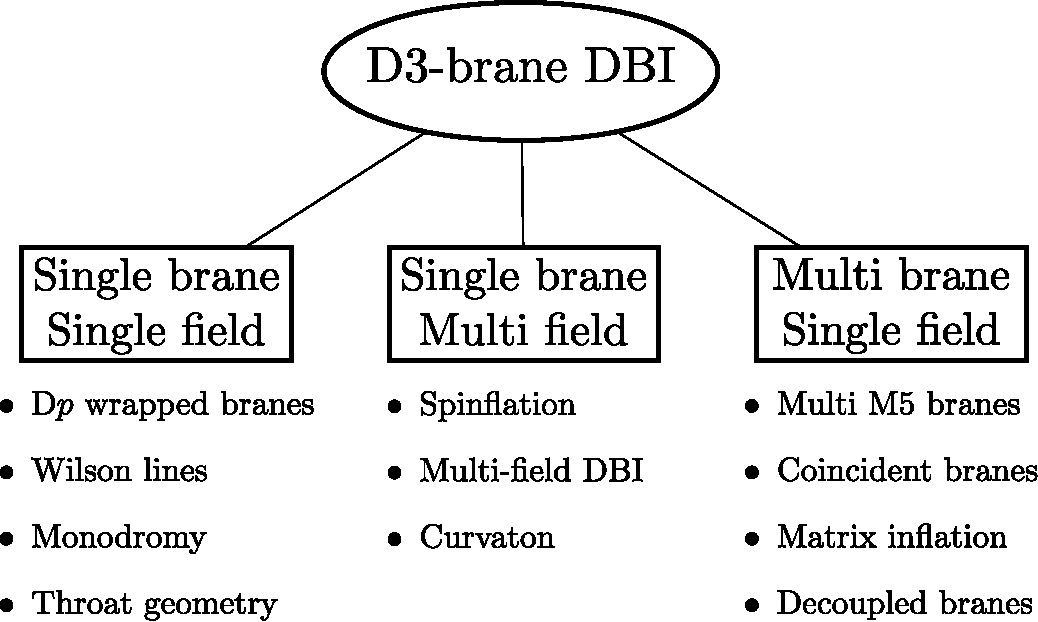
\includegraphics[width=0.8\textwidth]{./dbi/graphs/dbi-review.pdf}
 % dbi-review.pdf: 498x327 pixel, 72dpi, 17.57x11.54 cm, bb=0 0 498 327
 \caption[Recent DBI Inspired Models]{A schematic of recent DBI inspired models}
 \label{fig:review-dbi}
\end{figure}
% 

We have found that the standard DBI model appears to be in conflict with
observations. Many attempts have since been made to modify the original scenario in
order to evade the bounds derived above. These new models can be classified according
to
whether they involve single or multiple fields and single or multiple branes.
Figure~\ref{fig:review-dbi} lists some of the models in
each category.


The most straightforward extensions of the DBI model are single field, single brane
models. 
These have a single degree of freedom, as in the D3-brane model, but
they rely on other physical mechanisms to ease the bounds on $r$.
A natural extension to the single ${\rm D3}$-brane model 
is to consider a ${\rm D}p$-brane wrapped around a $(p-3)$-cycle of the 
internal space.
This leads to a change in the relationship
between $\rho$ and $\vp$ from that defined in Section~\ref{sec:dbiinflation}
\cite{Kobayashi:2007hm, Becker:2007ui, Ward:2007gs}.  
For example, Becker \etal \cite{Becker:2007ui} 
have proposed a model in which inflation is driven by a wrapped ${\rm D5}$-brane. 
In this case, the range of allowed values for the inflaton 
becomes independent of the throat charge, $N$, which weakens the upper bound on 
the tensor-scalar ratio to $r \lesssim 0.04$. (Strictly speaking there is a weak
dependence on the charge since $\Delta \varphi \sim N^{-1/4}$.)
However, in arriving at this bound, it was assumed that 
backreaction effects of any fluxes in the throat were 
negligible. 
Kobayashi \etal \cite{Kobayashi:2007hm} 
considered both ${\rm D5}$ and
${\rm D7}$ wrapped brane models, but concluded that the former case
required an excessively large background charge in 
order to relax the bounds on $r$. 
% 
This requirement is highly constraining, but is
still not as restrictive as the value of the charge required by the single brane scenario,
which effectively rules this model out. 
% 
Thus, a wrapped brane configuration is preferable to
the single D3-brane model, but the parameter space of the former is still severely
limited by the WMAP5 observations \cite{Alabidi:2008ej}. 
% However
% the difficulty in these models is that the backreaction is no longer under
% control. 


Another interesting proposal is warped Wilson line DBI. In this scenario, moduli
fields associated with Wilson
lines play the role of the inflaton \cite{Avgoustidis:2008zu}. This scenario is
T-dual to the
standard DBI model with non-parallel branes. In general, the model describes the
physics of a single brane with multiple position fields and multiple Wilson line
fields.
% 
In \Rref{Avgoustidis:2008zu}, observational predictions were derived for
the case when the brane position is fixed and only one Wilson line degree of freedom
is used. This implementation is therefore a single brane, single field model.
% 
By following the method outlined in Section~\ref{sec:upper-dbi} for this single field model,
a lower bound on $r$ was derived, instead of the upper bound \eqref{eq:upperbound}
\cite{Avgoustidis:2008zu}. The lower bound \eqref{eq:lowerbound} remains valid for
this scenario. 
% 
There are, therefore, two lower bounds on $r$ and the inconsistency of the
standard DBI model is not replicated. 
 


Changing the physical setting can also allow larger field ranges, which in turn can relax the
bounds on $r$. One such example is the case of a D4-brane in compactified manifolds
containing monodromies. 
The large field variations in this single brane, single field model lead to possibly
observable
tensor modes
\cite{Silverstein:2008sg}. Although formulated in Type IIA string theory, the
monodromy scenario has a simple inflationary interpretation as a large field, slow roll
model with a potential $V(\vp)\propto\vp^{2/3}$. 

The tensor-scalar ratio and other observable quantities are
significantly altered if the throat geometry is not of the $AdS_5$ type, even in the case of the
standard D3-brane model \cite{Gmeiner:2007uw}. In
\Rref{Butti:2004pk}, a one parameter family of solutions was found, which interpolates
between the
Klebanov-Strassler (KS) \cite{ks} and Maldacena-Nu\~{n}ez
\cite{Maldacena:2000yy} throats. As the throat geometry moves away from KS, more
non-Gaussianity is produced whereas the tensor-scalar ratio is reduced.
The choice of throat geometry, therefore, could affect the bounds on $r$
and must be considered when models are compared.



The next class of models that can be investigated are the single brane, multi-field
configurations. 
% 
The warped throat is six-dimensional, so it is natural to consider cases where
the D3-brane is not restricted to a radial trajectory. This was investigated in
Refs.~\cite{spinflation} and \cite{Huang:2007hh}. Increasing the degrees of
freedom in this way introduces the possibility of entropy mode production. There are also
changes in the predictions for the amount and type of non-Gaussianity produced
and the constraints on $r$ can be eased \cite{Arroja:2008yy, Langlois:2009ej,
Langlois:2008qf, Langlois:2008wt, Mizuno:2009mv, Mizuno:2009cv, RenauxPetel:2009sj}.
%
The bounds on $r$ could also be affected if a non-negligible part of the
curvature perturbation was produced by a curvaton field \cite{Lyth:2001nq}.
Curvaton fields arise generically in scenarios containing warped throats,
particularly for propagation near the tip \cite{Li:2008fm, Kobayashi:2009cm}. 
% 
% Differences in
% the bi- and tri-spectra could enable multi-field DBI models to be distinguished
% from single field ones. In particular multi-field DBI models
% have a unique tri-spectrum term with amplitude proportional to $\fnlloc\fnleq$
% \cite{RenauxPetel:2009sj}. This opens the possibility of a distinct
% observational signature for this type of model.
% 

Investigations have also been made into models with multiple branes, each of which
has a single dynamical field. In Refs.~\cite{Cai:2008if} and \cite{Cai:2009hw}, no
interactions between branes were considered, and the branes could conceivably propagate in different
throats. The action for $n$ decoupled branes in the
relativistic limit is the sum of $n$ copies of the DBI action
\eqref{eq:DBIaction-dbiintro}. The power spectrum of curvature perturbations is
enhanced by a factor of $n^{3/2}$ with respect to the single brane case. Consequently, the value
of the tensor-scalar ratio will be reduced. 


We have not yet addressed models with multiple branes but only one effective
degree of freedom. Multiple M5-branes in M-theory act with an effective
single degree of freedom, but the Lyth bound is now significantly weakened. Large
field ranges and an observable tensor signal are therefore possible \cite{Krause:2007jr}. 
Another proposal is that of $n$ D3-branes which are coincident and propagating in a
warped throat \cite{thomasward, hltw, Ward:2007gs, Berndsen:2009ww}. The
non-Abelian nature of the interactions between the branes differentiates this model
from other multi-brane models and the model is also known as ``Matrix Inflation''.
In Chapter~\ref{ch:multibrane} we
investigate this model in the relativistic limit
for both large and small $n$, and show how the constraints derived in this
chapter can be applied.


% 
% 
% 
% % % % % % % % % % % % % % % % % % % % % % % % % % % % % % % % 
% =========================================================== %
\section{Discussion}
\label{sec:conclusion-dbi}
% =========================================================== %
% % % % % % % % % % % % % % % % % % % % % % % % % % % % % % % % 

In this chapter, we have derived an upper limit on
the amplitude of the primordial gravitational wave spectrum
generated during UV DBI inflation. We considered   
the maximal inflaton field variation   
that can occur during the observable stages of inflation and assumed  
only that the brane was propagating inside the throat during that epoch. 
The bound (\ref{eq:upperbound}) is valid for an arbitrary inflaton potential and 
warp factor (modulo some weak caveats) and can be expressed 
entirely in terms of observable parameters, once the volume of 
the five-dimensional sub-manifold of the throat has been specified. 
The inferred upper limit on $r$ is surprisingly strong. 
We find that the standard UV  
scenario predicts tensor perturbations that are undetectably small, 
at a level ${r_*} \lesssim {10^{-7}}$. 

The current WMAP5 data 
favours models that generate a red spectral index, $n_s<1$,
when both the gravitational waves and running in the scalar 
spectral index are negligible. For UV versions of the scenario, 
we have identified a corresponding 
lower limit on $r$ which applies in this region of 
parameter space, $r_* \gtrsim 0.1 (1-n_s)$. It is clear that 
the standard scenario 
cannot satisfy both the upper and lower bounds 
on the tensor modes for the observationally favoured value 
$1-n_s \simeq 0.03$.


The generality of our 
analysis implies that modifying either the inflaton potential 
or the form of the warp factor is unlikely to resolve this discrepancy. 
On the other hand, there are a number of possible ways of reconciling  
theory with observation. In general, 
either the upper or lower limit on $r$ needs to be relaxed. 
Weakening the latter would require a violation of the slow roll 
conditions or a blue spectral index. 
A value of $n_s >1$ is compatible with WMAP5 if the running of the 
spectral index 
is sufficiently negative, but is only marginally
consistent if just the tensor modes are non-negligible.  The 
upper limit on $r$ can be weakened by reducing 
the volume of $X_5$ or 
by generalising the DBI action. Furthermore, it need not necessarily 
apply in IR versions of the scenario, although the BM bound will still hold
in such cases. 
We considered a generalised version of the 
DBI action and identified a necessary condition on the form of such  
an action for the BM bound to be relaxed.

% As a concrete example, 
% we investigated a version of IR inflation that is driven by 
% multiple coincident branes and found that  
% the bounds on the tensor-scalar ratio can indeed 
% be made compatible if the brane charges satisfy appropriate 
% conditions.   





In conclusion therefore, we have shown that primordial gravitational wave constraints 
combined with cosmological observations of the density perturbation
spectrum act as a powerful discriminant of DBI inflationary models. 
They also serve as an important observational guide for identifying viable 
generalisations of the scenario. In Chapter~\ref{ch:multibrane} we will explore
one particular generalisation, the multi-coincident brane scenario
introduced in \Rref{thomasward}.

% 
% % % % % % % % % % % % % % % % % % % % % % 
% multibrane.tex - Ian Huston
% $Id: multibrane.tex,v 1.7 2009/07/14 17:23:04 ith Exp $
% % % % % % % % % % % % % % % % % % % % % 
% Redefine CVSRevision for this section
\renewcommand{\CVSrevision}{\version$Id: multibrane.tex,v 1.7 2009/07/14 17:23:04 ith Exp $}

% % % % % % % % % % % % % % % % % % % % % % % % % % % % % % % % 
% =========================================================== %
% % % % % % % % % % % % % % % % % % % % % % % % % % % % % % % % 
\chapter{Multi brane inflation}
\label{ch:multibrane}
% % % % % % % % % % % % % % % % % % % % % % % % % % % % % % % % 
% =========================================================== %
% % % % % % % % % % % % % % % % % % % % % % % % % % % % % % % % 

% % % % % % % % % % % % % % % % % % % % % % % % % % % % % % % % 
% =========================================================== %
% % % % % % % % % % % % % % % % % % % % % % % % % % % % % % % % 
\section{Introduction}
\label{sec:multi-intro}
% % % % % % % % % % % % % % % % % % % % % % % % % % % % % % % % 
% =========================================================== %
% % % % % % % % % % % % % % % % % % % % % % % % % % % % % % % % 

The quest to realise inflation within string/M-theory continues to 
attract considerable attention. The Dirac-Born-Infeld (DBI) scenario 
of the compactified type IIB theory is a well-motivated model, 
in which inflation is driven by one or more ${\rm D}$-branes 
propagating in a warped `throat' background
\cite{brane1,brane11,brane12,brane13,brane2,brane20,brane3,brane4,brane5,brane6}
. Such a background is generated 
by the non-trivial form-field fluxes over the internal dimensions. 
(For recent reviews, see
\cite{tyereview,McAllister:2007bg,Lorenz:2007ze,Kallosh:2007wm,Bean:2007eh,bean,
cline}.) 
In the simplest version of the scenario, 
the inflaton parametrizes the radial 
position in the throat of a single ${\rm D3}$-brane. 
The brane dynamics are determined by the DBI action in such a 
way that the inflaton's kinetic energy is bounded from above by the warped 
brane tension. The regime where this bound is nearly saturated is 
known as the `relativistic' limit.

Recently relativistic DBI inflation has come under considerable 
pressure when confronted with cosmological observations.  
Baumann \& McAllister (BM) and Lidsey \& Huston (LH) 
have shown that the ratio of the amplitudes of the 
tensor and scalar perturbations generated during 
inflation is bounded from above by $r \lsim 10^{-7}$
\cite{bmpaper,lidseyhuston}. 
However in ultra-violet (UV) versions of the scenario, where 
the ${\rm D}$-brane is moving towards the tip of the throat, the tensor-scalar 
ratio is also bounded from below, $r \gsim 0.1 (1-n_s)$, 
where $n_s$ denotes the spectral index 
of the scalar perturbation spectrum \cite{lidseyhuston}. 
The two bounds on $r$ are incompatible 
if $n_s \sim 0.95$, as currently favoured by Cosmic Microwave Background 
(CMB) observations \cite{spergel,Komatsu:2008hk}. 

The purpose of the present paper is to investigate whether the 
upper bounds on $r$ can be relaxed in more general DBI 
inflationary scenarios. 
A natural extension to the single ${\rm D3}$-brane model 
is to consider a ${\rm D}p$-brane wrapped around a $(p-3)$-cycle of the 
internal space. For example, Becker \etal \cite{Becker:2007ui} 
have proposed a model where inflation is driven by a ${\rm D5}$-brane. 
In this case, the range of allowed values for the inflaton 
becomes independent of the throat charge, $N$, which weakens the upper bound on 
the tensor-scalar ratio to $r \lsim 0.04$. Strictly speaking this is 
only true for the ${\rm D7}$-brane case, since the
wrapped ${\rm D5}$-brane imposes 
$\Delta \phi \sim N^{-1/4}$.
However in arriving at this bound, it was assumed that the 
backreaction effects of any fluxes in the throat were 
negligible. Kobayashi \etal \cite{Kobayashi:2007hm} 
considered both ${\rm D5}$- and
${\rm D7}$-brane models, but concluded that the former case
required an excessively large background charge in 
order to relax the bounds on $r$. Whilst this is highly constraining, it is still much better than
the
case for single ${\rm D3}$-branes which require a much higher background charge - and therefore are
effectively ruled
out as a predictive model. Thus wrapped brane configurations are preferable to single brane models.
However
the difficulty in these models is that the backreaction is no longer under control.

Alternative ways to relax these bounds have been proposed, including
theories based upon multi-field models \cite{Huang:2007hh}, the addition of
angular momentum as another degree of freedom \cite{spinflation} and using
different throat geometries \cite{Gmeiner:2007uw}. However it must be noted that
the extra degrees of freedom introduced in these models do not solve the problem. The 
bounds are relaxed only by a small fraction, and therefore these models should still be 
regarded as being unsatisfactory since they require an extreme amount of fine tuning in order
to work.

Another alternative possibility is to consider 
multiple brane configurations\footnote{In certain limits this approach 
is actually dual to considering wrapped branes \cite{Ward:2007gs}.}. 
In the case where  
$n$ branes are localised initially at equal distances $l > l_s$ and 
subsequently follow the same trajectory, 
the effective theory is equivalent to that of $n$ copies of the
action for a single brane. A more general initial condition, particularly
for branes created in the infra-red (IR) region of the throat
\cite{brane13, DeWolfe:2004qx, Kachru:2002gs}, is that
the branes should be separated over a range of scales, 
with a subset being coincident and the remainder being widely separated. 

Our approach in this paper is two-fold. We 
begin in Sections \ref{sec:noncanoninfl} and \ref{sec:theobound} 
by noting that the upper bounds on the tensor-scalar ratio arise due to the
special algebraic properties of the DBI action. We 
then adopt a phenomenological approach in Section \ref{sec:relaxingbound}
and identify a general class of non-canonical inflationary models, 
where the leading-order contribution to the non-Gaussianity of the 
curvature perturbation is determined 
entirely by the speed of sound of the inflaton fluctuations. 
In these models, the bounds on $r$ can be relaxed 
if significant non-Gaussianities are generated.  
This class of models includes the relativistic limit  
of the action for $n$ coincident ${\rm D3}$-branes, 
which originates from a UV complete theory. This motivates us 
to develop the theory of multiple coincident branes further in Section
\ref{sec:multibranes}. We find that for a finite number of branes, 
the effective action for $n$ coincident branes can be derived and the backreaction
kept firmly under control.
In Section \ref{sec:multibounds} we find that such models 
can in principle lead to a detectable 
gravitational wave background if 
the number of coincident branes is sufficiently small. 

Units are chosen such that $\hbar = c =1$ and $\Mpl \equiv (8\pi G)^{-1/2}
= 2.4 \times 10^{-18} \, {\rm GeV}$ denotes the 
reduced Planck mass. 

% % % % % % % % % % % % % % % % % % % % % % % % % % % % % % % % 
% =========================================================== %
% % % % % % % % % % % % % % % % % % % % % % % % % % % % % % % % 
\section{Non-Canonical Inflation} 
\label{sec:noncanoninfl}
% % % % % % % % % % % % % % % % % % % % % % % % % % % % % % % % 
% =========================================================== %
% % % % % % % % % % % % % % % % % % % % % % % % % % % % % % % % 


The low-energy, world-volume dynamics of a 
${\rm D3}$-brane in a warped background is determined 
by an effective action of the form 
\begin{equation}
\label{DBIaction}
S=\int  d^4x \sqrt{|g|} \left[ \frac{\Mpl^2}{2} R 
+ P (\phi , X) \right] \,,
\end{equation}
where $R$ is the Ricci curvature scalar, 
$X \equiv -\frac{1}{2}g^{\mu \nu}\nabla_\mu \phi \nabla_\nu \phi$
denotes the kinetic energy of the inflaton field $\phi$, and the function  
$P (\phi , X)$ is referred to as the `kinetic function'.  

We assume that the four-dimensional universe is   
spatially flat and isotropic and sourced by an  
homogeneous inflaton field, $\phi =\phi (t)$, with energy 
density $E = 2X\PX - P$, where a subscripted comma denotes partial
differentiation. 
We further assume that the inflaton dynamics  
generates a quasi-exponential expansion of the universe, 
where $\epsilon \equiv -\dot{H}/H^2 \ll1$. 
 
It proves convenient to define two parameters in terms of the 
kinetic  function $P$ and its derivatives \cite{lidser1,lidser3}: 
\begin{eqnarray}
\label{defcs}
 c_s^2 \equiv \frac{\PX}{\PX + 2X P_{,XX}} \,,
\\
\label{deflambda}
\Lambda \equiv  \frac{X^2 P_{,XX} +
\frac{2}{3}X^3 P_{,XXX}}{X P_{,X} +
2X^2 P_{,XX}}\,.
\end{eqnarray}
The first parameter, $c_s$, determines the sound speed of fluctuations 
in the inflaton field. This can be significantly less than unity, 
in contrast to slow-roll inflation driven by a canonical 
field such that $P_{,X} =1$.

The amplitudes of the scalar and tensor perturbations 
generated during inflation are given by \cite{gm}
\begin{eqnarray} 
\label{eqn:Ps2}
 \Ps = \frac{H^4}{8\pi^2 X}\frac{1}{c_s \PX} \,,
\\
\label{eqn:Pt2}
\Pt = \frac{2}{\pi^2} \frac{H^2}{\Mpl^2} \,,
\end{eqnarray}
respectively, and the ratio of these amplitudes 
is defined as \cite{gm} 
\begin{equation}
\label{defr}
r\equiv \frac{\Pt}{\Ps} = 16c_s \epsilon \,.
\end{equation}  
The WMAP3 normalization of the CMB power spectrum 
implies that $\Ps= 2.5\times10^{-9}$ and 
the experimental upper bound on the tensor-scalar 
ratio is $r <0.55$ \cite{spergel}.

Deviations from Gaussian statistics in the curvature perturbation, ${\cal{R}}$,
are parametrized in terms of the non-linearity parameter, 
$\fnl$, which is defined by ${\cal{R}} = {\cal{R}}_G + \frac{3}{5} \fnl  (
{\cal{R}}_G^2 -\langle {\cal{R}}_G^2 \rangle )$, where the 
quadratic component represents a convolution and 
${\cal{R}}_G$ denotes the Gaussian contribution \cite{maldacena}. In the limit  
where the three momenta have equal magnitude (corresponding to the equilateral  
triangle limit), the leading-order contribution to the non-linearity 
parameter is given by \cite{chenetal,lidser3}
\begin{equation} 
\label{deffnl}
 \fnl = -\frac{35}{108}\left(\frac{1}{c_s^2} -1 \right) +
\frac{5}{81}\left( \frac{1}{c_s^2} -1 -2\Lambda \right) \,.
 \end{equation} 
One should note that the sign convention is that employed
by the WMAP data set.
Data from WMAP3 imposes the bound $|\fnl| < 300$ on this parameter
\cite{spergel}. The corresponding bounds for other triangle configurations 
may be much tighter than this and this may be particularly relevant if 
non-Gaussian signatures have indeed been detected in the 
CMB \cite{Yadav:2007yy,crim}. The more recent WMAP5 data set
\cite{Komatsu:2008hk} improves on this bound somewhat, and
also indicates that it is distinctly asymmetric. At the $95 \%$ confidence level, the bound on the 
equilateral triangle becomes $-151 < \fnl < 253$.

Eqs. (\ref{eqn:Ps2}) and (\ref{eqn:Pt2}) imply 
that the variation of the inflaton field during inflation  
is related to the tensor-scalar amplitude by \cite{lyth,bmpaper}
\begin{equation}
\label{genlythbound}
\frac{1}{\Mpl^2}
\left( \frac{d \phi}{d \cal{N}} \right)^2 = \frac{r}{8 c_s P_{,X}} \,,
\end{equation}
where ${\cal{N}} \equiv \int dt \, H$ denotes the number of e-foldings.
We will refer to the epoch of inflation that can be directly 
constrained by cosmological observations as 
`observable inflation' and will assume that this phase 
occurred when the brane was located within a 
throat region\footnote{We denote the values of all parameters 
evaluated during observable inflation by a subscript 
`$*$'.}. Observable inflation corresponds to no more than about 4 e-foldings  
of inflationary expansion, $\Delta {\cal{N}}_* \simeq 4$. 
The total variation in the inflaton field between the epoch of observable 
inflation and the end of inflation is then given by
\begin{equation}
\label{totalfield}
\frac{\Delta \phi_{\rm inf}}{\Mpl} = 
\left( \frac{r}{8c_sP_{,X}} \right)_*^{1/2} {\cal{N}}_{\rm eff} \,,
\end{equation}
where
\begin{equation}
\label{Neff}
{\cal{N}}_{\rm eff} \equiv \left( \frac{c_sP_{,X}}{r}\right)_*^{1/2}
\int_0^{{\cal{N}}_{\rm end}}  
\left( \frac{r}{c_sP_{,X}} \right)^{1/2} d {\cal{N}} \,.
\end{equation}
If $r/(c_s P_{,X})$ varies 
sufficiently slowly during observable inflation, 
the corresponding change in the value of the inflaton  
field is given approximately by \cite{lyth,bmpaper}
\begin{equation}
\label{approxlyth}
\left( \frac{\Delta \phi}{\Mpl} \right)_*^2 \simeq 
\frac{(\Delta {\cal{N}}_*)^2}{8} \left( \frac{r}{c_sP_{,X}} \right)_* \,.
\end{equation}

% 
% 
% % % % % % % % % % % % % % % % % % % % % % % % % % % % % % % % 
% =========================================================== %
% % % % % % % % % % % % % % % % % % % % % % % % % % % % % % % % 
\section{Theoretic Upper Bounds on the Tensor-Scalar Ratio}
\label{sec:theobound}
% % % % % % % % % % % % % % % % % % % % % % % % % % % % % % % % 
% =========================================================== %
% % % % % % % % % % % % % % % % % % % % % % % % % % % % % % % % 

The ten-dimensional metric of the warped deformed conifold inside a  
throat region has the form 
\begin{equation}
\label{conemetric}
ds_{10}^2= h^2 ( \rho) ds_4^2 + h^{-2} (\rho ) 
\left( d\rho^2 +\rho^2 ds_{X_5}^2 \right) \,,
\end{equation} 
where the `warp factor' $h(\rho )$ is a function of the radial 
coordinate $\rho$ along the throat and $X_5$ denotes a five-dimensional, 
Sasaki-Einstein manifold. In many scenarios, the ten-dimensional 
manifold (\ref{conemetric}) can be approximated by the product 
$AdS_5 \times X_5$, where $AdS_5$ represents five-dimensional, 
anti-de Sitter space. In this case, the warp factor is given by  
\begin{equation}
h = \frac{\rho}{L} , \qquad 
L^4 = \frac{4\pi^4 g_s N}{\Vol m_s^4}\,,
\end{equation} 
where $L$ denotes the $AdS_5$ radius of curvature, 
$\Vol$ is the volume of the five-manifold $X_5$ with unit radius, 
$N$ is the ${\rm D3}$-brane charge in the throat, 
$g_s$ is the string coupling and $m_s$ is the string mass scale. 
Generally the value of the inflaton field 
is determined by the radial position of the 
${\rm D3}$-brane in the throat, 
$\phi \equiv \rho \sqrt{T_3}$, where $T_3 \equiv  
m_s^4/[(2\pi)^3g_s]$ is the brane tension. 

The four-dimensional Planck mass is related to the volume 
of the compactified Calabi-Yau three-fold, $V_6$, such that
$\Mpl^2 =V_6 \kappa_{10}^{-2}$, where $\kappa_{10}^2 \equiv \frac{1}{2}
(2 \pi )^7 g_s^2/ m_s^{8} = \pi /T_3^{2}$ for a 
${\rm D3}$-brane \footnote{We parameterise the Planck scale 
in terms of the ${\rm D3}$-brane tension out of convenience, 
and note that there is no physical relationship between the two.}. 
Hence the Planck mass is bounded from 
below by the volume of a throat region, 
$\Mpl^2 >V_{6,{\rm th}} \kappa_{10}^{-2}$, 
where $V_{6,{\rm th}} \lsim V_6$ denotes the throat volume. 
For an $AdS_5 \times X_5$ throat, Baumann \& McAllister (BM)
exploited this inequality to derive an upper limit on the 
maximum variation of the inflaton field in the throat, 
$\Delta \phi_{\rm max} < 2\Mpl/\sqrt{N}$, which leads to the 
corresponding limit $|\Delta \phi |_* < 2\Mpl /\sqrt{N}$ \cite{bmpaper}.  
Combining this with the constraint (\ref{approxlyth}) therefore 
yields an upper limit on the tensor-scalar ratio: 
\begin{equation}
\label{BMbound}
r_* < \frac{32}{N {\cal{N}}_{\rm eff}^2} \left( 
c_s P_{,X} \right)_* \,.
\end{equation}

Two of the authors (Lidsey \& Huston, LH) derived a complementary bound on the 
tensor-scalar ratio by noting that during observable inflation
the brane spans a fraction of the throat volume \cite{lidseyhuston}
\begin{equation}
\label{approxvol}
| \Delta V_{6,*} | \simeq \Vol \frac{| \Delta \rho_*| \rho_*^5}{h_*^4}
\end{equation}
and, since $| \Delta V_{6,*} |< 
V_{6,{\rm th}}$, it follows that 
\begin{equation}
\label{firstbound}
\left(\frac{\Delta \phi}{\Mpl}\right)^2_* < \frac{T_3 \kappa_{10}^2
(\Delta \rho_*)^2}{| \Delta V_{6*}|} \,.
\end{equation}
It was then assumed that the fractional change in the value of the 
inflaton field during observable inflation was less than unity:
\begin{equation}
\label{delta1constraint}
|\Delta \phi_* | <  \phi_* \,.
\end{equation} 
This condition is necessarily satisfied in UV
versions of the scenario, 
where the brane is moving towards the tip of the throat, but must be 
assumed as a further constraint in IR versions 
where the brane moves out of the throat, since in these latter cases
$\phi_*$ could be very small. Combining the limit 
(\ref{delta1constraint}) with Eq. (\ref{approxvol}) then implies that 
\begin{equation}
| \Delta V_{6,*} | > \Vol \frac{( \Delta \rho_* )^6}{h_*^4}
\end{equation}
and substituting this constraint into the bound (\ref{firstbound}) yields 
the condition 
\begin{equation}
\left( \frac{\Delta \phi}{\Mpl} \right)_*^6 < \frac{\pi T_3}{\Vol} 
\left( \frac{h_*}{\Mpl} \right)^4 \,.
\end{equation}
Finally substituting the constraint (\ref{approxlyth}) 
yields the upper limit \cite{lidseyhuston}
\begin{equation}
\label{LHbound}
r_* < \frac{10}{(\Delta {\cal{N}})_*^2} \left( \frac{T_3}{\Vol} \right)^{1/3} 
\left( \frac{h_*}{\Mpl} \right)^{4/3} \left( c_s P_{,X} \right)_* \,.
\end{equation}

Comparison of the limits (\ref{BMbound}) and (\ref{LHbound})
implies that the LH bound is the stronger of the two when
\begin{equation}
\label{LHstronger}
h_*^{4/3}N < 20 \left( \Vol g_s \right)^{1/3}  
\left( \frac{m_s}{\Mpl} \right)^{-4/3} 
\frac{( \Delta {\cal{N}} )_*^2}{{\cal{N}}^2_{\rm eff}} \,.
\end{equation}
For typical field-theoretic values $\Vol \simeq \mathcal{O}(\pi^3)$, $m_s \sim
0.1 \Mpl$ 
and  $g_s \sim 10^{-2}$, this implies 
\begin{equation}
\label{LHstronger1}
h_*^{4/3} N < 300 \frac{(\Delta {\cal{N}})^2_*}{{\cal{N}}_{\rm eff}^2} \,.
\end{equation}

In the following Section, we identify a class of models in which  
these bounds could be relaxed. 
% 
% 
% % % % % % % % % % % % % % % % % % % % % % % % % % % % % % % % 
% =========================================================== %
% % % % % % % % % % % % % % % % % % % % % % % % % % % % % % % % 
\section{Relaxing the Upper Bounds on the Tensor-Scalar Ratio}
\label{sec:relaxingbound}
% % % % % % % % % % % % % % % % % % % % % % % % % % % % % % % % 
% =========================================================== %
% % % % % % % % % % % % % % % % % % % % % % % % % % % % % % % % 
% 

In the standard DBI scenario, the kinetic function defined in 
Eq. (\ref{DBIaction})  takes the form 
\begin{equation}
\label{DBIkinetic}
P (\phi , X) = -T(\phi ) \sqrt{1-2T^{-1}(\phi ) X} + T(\phi ) - V(\phi ) \,,
\end{equation}
where $T(\phi ) = T_3 h^4 (\phi )$ 
is the warped brane tension and  $V(\phi )$ is the 
inflaton potential. 
Typically in warped compactifications of 
IIB supergravity, this potential is determined by the 
relevant fluxes and brane interaction terms. 
We will ignore the precise origin
and form of this potential, but simply
note that it is highly sensitive to the string theoretic construction. For the
purpose of this note we will simply treat it 
as an arbitrary function of the inflaton field.
(See, for example, Ref. \cite{brane5} for a discussion 
on the precise form that the inflaton potential may take.)

The standard DBI scenario (\ref{DBIkinetic}) is algebraically special, 
in the sense that the kinetic function satisfies the constraints 
\begin{equation}
\label{special}
c_s P_{,X} = 1 , \qquad  \Lambda = \frac{1}{2} \left( 
\frac{1}{c_s^2} -1 \right) \,.
\end{equation}
It follows that the 
bounds (\ref{BMbound}) and (\ref{LHbound}) 
on the tensor-scalar ratio could in principle be 
significantly relaxed in models where $(c_sP_{,X})_* \gg 1$. 
In view of the second relation in Eq. (\ref{special}), it is of interest 
to take a phenomenological approach and consider the more  
general class of models where 
\begin{equation}
\label{defalpha}
\frac{1}{c_s^2} -1 = \alpha \Lambda \,,
\end{equation}
for some positive constant $\alpha$. Moreover since 
a large non-Gaussian signature in the curvature perturbation is 
typically generated in models where the sound speed of fluctuations 
is small, we will begin by considering 
scenarios where the kinetic function satisfies the 
inequalities: 
\begin{equation}
\label{Plimits}
X^2 P_{,XXX} \gg XP_{,XX} \gg P_{,X} \,.
\end{equation}

In these limits the constraint (\ref{defalpha}) reduces to the 
third-order, non-linear, partial differential equation
\begin{equation}
\label{pde}
P^2_{,XX} = \frac{\alpha}{6} P_{,X} P_{,XXX} \,.
\end{equation}
Changing the dependent variable to $Q \equiv P_{,XX}/P_{,X}$ 
reduces Eq. (\ref{pde}) to 
\begin{equation}
\label{Qequation}
\alpha Q_{,X} = (6-\alpha )Q^2 \,,
\end{equation}
and it is straightforward to integrate Eq. (\ref{Qequation}) 
exactly. The remaining integrations can also be performed analytically 
and the general solution to Eq. (\ref{pde}) for $\alpha \ne
6$ is given by\footnote{The special case $\alpha =6$ results in an 
exponential dependence of the kinetic function on $X$, and is 
therefore an example of a higher-derivative theory. However we 
do not consider this model further, since it does not lead to a 
weakening of the gravitational wave constraints.}
\begin{equation}
\label{gensol}
P (\phi , X) = f_1 (\phi ) \left[ 1-f_2 (\phi ) X 
\right]^m -f_3(\phi ) \,,
\end{equation}
where $f_i (\phi )$ are arbitrary functions of the scalar 
field and 
\begin{equation}
m \equiv \frac{2(\alpha -3 )}{\alpha -6} \, . 
\end{equation}
It can be verified that the inequalities (\ref{Plimits}) 
are satisfied in the `relativistic' limit, where $X \simeq 1/f_2$.
We consider the inflationary dynamics in this limit in what follows. 
For completeness, we note that Eq. (\ref{defalpha}) can be solved 
analytically in 
full generality and the solution is presented in the Appendix. 

The standard DBI scenario is recovered for $m=1/2$. 
More generally however, Eq. (\ref{gensol}) implies that  
\begin{eqnarray}
\label{consequence1}
c_sP_{,X} \simeq -\frac{m f_1 f_2}{\sqrt{2(1-m)}} \left( 
1- f_2X \right)^{(2m-1)/2} \,,
\\
c_s^2 \simeq \frac{1-f_2X}{2(1-m)} \,,
\end{eqnarray}
when $X \simeq 1/f_2$. Self-consistency therefore
requires $m<1$. Moreover
we find from Eq. (\ref{deffnl}) that 
\begin{eqnarray}
\label{consequence3}
\fnl \simeq \frac{-\beta}{1-f_2X} , \qquad \beta \equiv \frac{5(59-55m)}{486}
\,,
\\
\label{consequence4}
\fnl \simeq -\frac{\sigma}{c_s^2}, \qquad \sigma \equiv 
\frac{5}{972} \left( \frac{59-55m}{1-m} \right) \,.
\end{eqnarray}
Hence substituting Eqs. (\ref{consequence1}) and (\ref{consequence3}) 
into the BM bound (\ref{BMbound}) and the LH bound (\ref{LHbound}) implies that 
\begin{equation}
\label{weakBMbound}
r_*< \frac{32}{N {\cal{N}}_{\rm eff}^2} \frac{(-m) f_1 f_2}{\sqrt{2(1-m)}}
\left( -\frac{\fnl}{\beta} \right)^{(1-2m)/2}
\end{equation}
and 
\begin{equation}
\label{weakLHbound}
r_* < \frac{10}{(\Delta {\cal{N}})_*^2} \left( \frac{T_3}{\Vol} \right)^{1/3} 
\left( \frac{h_*}{\Mpl} \right)^{4/3}
\frac{(-m) f_1 f_2}{\sqrt{2(1-m)}}
\left( -\frac{\fnl}{\beta} \right)^{(1-2m)/2}
\end{equation}
respectively. 

We conclude, therefore, that 
the upper limit on the tensor-scalar ratio could be significantly 
relaxed if $m <1/2$, since the non-linearity parameter is at present only 
weakly constrained at $\fnl >-151$. Although it is possible 
to phenomenologically construct a model which has a value of $m$ in this 
range, it is clearly preferable to identify  UV complete models
that satisfy this requirement within a string theory context. 
Unfortunately this is quite difficult to achieve since the inflaton 
will either be associated with an open or closed string mode. 
The open strings are governed by relativistic actions of the 
DBI form, whilst closed strings arise from compactification of Einstein gravity
and are typically put into canonical form.
However there do exist classes of open string
models which satisfy the above requirement, 
namely those associated with multiple coincident branes.

More specifically, if the branes are
spatially separated, the effective action is algebraically equivalent 
to that of a single brane. It will therefore not satisfy the 
bound on $m$ \footnote{In this discussion, we are ignoring 
the non-trivial backreaction of these branes on the background, and therefore 
one should be careful about the range of validity of the effective action.}. 
Similarly it was shown in \cite{thomasward}
that $n$ coincident branes, in the large $n$ limit, will also fall into 
this class of models. On the other hand, if it is assumed that 
$n$ is finite, the special properties associated with the 
matrix degrees of freedom become important and this 
results in a kinetic function satisfying $m \le 1/2$.
We will discuss this in more detail in the following Section.

% 
% 
% 
% % % % % % % % % % % % % % % % % % % % % % % % % % % % % % % % 
% =========================================================== %
% % % % % % % % % % % % % % % % % % % % % % % % % % % % % % % % 
\section{Action for Multiple Coincident Branes} 
\label{sec:multibranes}
% % % % % % % % % % % % % % % % % % % % % % % % % % % % % % % % 
% =========================================================== %
% % % % % % % % % % % % % % % % % % % % % % % % % % % % % % % % 


We have seen how the form of the kinetic function
$P$ can significantly change the
strength of the LH bound on the tensor-scalar ratio, depending on its explicit
form. One model in which a suitable form for 
$P$ is realised is the multiple coincident
brane model as outlined by Thomas \& Ward \cite{thomasward}.

The world-volume theory for coincident branes is not fully known, although
a number of proposals have been made. We will restrict our analysis to Myers' 
prescription, since this has been extensively discussed in the 
literature\footnote{There is also a proposal by Tseytlin \cite{Tseytlin}
for the non-Abelian theory of coincident D-branes.} \cite{myers1, myers2}. 
In general the open string degrees of freedom for $n$ coincident branes 
combine to fill out representations of $U(n)$ (as opposed to $U(1)^n$ 
in the case of separated branes). This introduces a non-Abelian 
structure into the theory. In the single brane case, the fluctuations of the 
brane are characterised by induced scalar fields on the world-volume. 
However for multiple branes
these scalars must be promoted to matrix representations of some gauge group. 

Typically the transverse space of any given compactification will always admit
an $SO(3)$ isometry. We can therefore choose our scalars to 
transform under representations of the algebra of $SO(3) \sim SU(2)$ by making 
the identifications
\begin{equation}
\phi^i = R \alpha^i \hspace{1cm} i =1,  \ldots 3 \,,
\end{equation}
where $R$ is some scale with canonical mass dimension, and the $\alpha^i$ are
specified to be the irreducible generators satisfying the commutator
\begin{equation}
[\alpha^i, \alpha^j] = 2i \epsilon_{ijk} \alpha^k \,,
\end{equation}
and the conditions
\begin{equation}
\frac{1}{n} Tr(\alpha^i \alpha^j) = \hat{C} \delta^{ij} = (n^2-1) \delta^{ij}
\,,
\end{equation}
where $\hat{C}$ is the quadratic Casimir of the gauge group.
The irreducibility condition corresponds to the configuration being in the
lowest energy state. It is therefore an additional fine-tuning
of the initial conditions. 

The Myers prescription requires a symmetrised trace (denoted $STr$) to 
be made over the gauge group. This implies that 
the symmetric averaging must be taken over all the group dependence 
before taking the trace. For $n \gg 1$, the symmetric trace can be approximated with a trace, 
which results in the usual DBI action multiplied by a potential term (as
described in \cite{thomasward, Kachru:2002gs}). 
However for finite $n$, the symmetrisation clearly becomes more important and it is essential that
we
have some means of performing this operation. Recently
a prescription for the symmetric trace at finite $n$ was proposed \cite{Ramgoolam:2004gw,
McNamara:2005ry}, 
using highest weight methods and chord diagrams. 

The result is that the $STr$ acts on different spin representations of $SU(2)$ 
in the following manner:
\begin{eqnarray}
STr (\alpha^i \alpha^i)^q = 2(2q+1)\sum_{i=1}^{n/2}(2i-1)^{2q} , 
\qquad n\; \mathrm{ even}\,, 
\\
STr (\alpha^i \alpha^i)^q = 2(2q+1)\sum_{i=1}^{(n-1)/2} (2i)^{2q} , 
\qquad n\; \mathrm{ odd}\,.
\end{eqnarray}

In order for the solution to converge in this prescription, 
it is also necessary to modify the definition of the radius of the 
$SU(2)$ sphere. In the large $n$ limit, this is given by
\begin{equation}
\rho^2 = \lambda^2 R^2 \frac{1}{n} Tr(\alpha^i \alpha^i) = \lambda^2 R^2
\hat{C} \,,
\end{equation}
where $\lambda \equiv 2\pi l_s^2 = 2\pi m_s^{-2}$, 
whereas for finite $n$, it becomes
\begin{equation}
\rho^2 = \lambda^2 R^2 \mathrm{Lim}_{q \to \infty} \left(\frac{STr (\alpha^i
\alpha^i)^{q+1}}{STr(\alpha^i \alpha^i)^q} \right) 
= \lambda^2 R^2 (n-1)^2 \,.
\end{equation}
This converges to the large $n$ result in the appropriate limit.
This point is important, since the warp factor 
of the four-dimensional theory is typically of the form $h= h(\rho)$.

The resulting kinetic function for $n$ coincident branes in 
the finite $n$ limit is therefore given by
\begin{equation}
\label{generalP}
P = -T_3 STr \left(h^4(\rho) \sum_{k,p=0}^{\infty}(-\XR)^k Y^p (\alpha^i
\alpha^i)^{k+p}{1/2 \choose k} {1/2 \choose p} + V(\rho)
-
h^4(\rho) \right) \,,
\end{equation}
where 
\begin{equation}
Z \equiv \lambda^2 h^{-4}(\rho), \hspace{0.5cm} Y \equiv 4\lambda^2 R^4
h^{-4}(\rho),
\hspace{0.5cm} {1/2 \choose q}
\equiv \frac{\Gamma(3/2)}{\Gamma(3/2-q)\Gamma(1+q)} \,.
\end{equation}
Note that the second and third terms in Eq. (\ref{generalP}) 
are singlets under the $STr$ and therefore contribute terms proportional 
to $n$. The physics of these branes away from the large $n$ limit is particularly interesting as
discussed further
in \cite{thomasward, Ward:2007gs}.

The simplest case to consider is that of two coincident branes. However
the form of the $STr$ prescription implies that all other solutions for 
$n>2$ can be deduced entirely from the $n=2$ solution by a recursion relation. 
In order to see this, let us define 
\begin{eqnarray}
\label{2brane}
P_2(Z,Y) &=& - 2 T_3 h^4 \left(\frac{(1+2Y -
(2+3Y)\XR)}{\sqrt{1+Y}\sqrt{1-\XR}}\right) \,, \nonumber \\
E_2(Z,Y) &=& 2 T_3 h^4 \left(\frac{(1+2Y -
Y\XR)}{\sqrt{1+Y}(1-\XR)^{3/2}}\right) \,.
\end{eqnarray}
These quantities correspond to the pressure and energy density functions 
when $n=2$ which arise solely from the DBI sector of the action.
The full pressure and energy densities are then 
given by $P = P_2 - 2T_3(V-h^4)$ and
$E = E_2 + 2T_3 (V-h^4)$, respectively.
Since the symmetrised trace acts differently on the differing spin
representations of $SU(2)$, we should expect this structure to follow
through in the recursion relation. Indeed, we find that for odd $n$
\begin{eqnarray}
\label{oddbrane}
P_n^{(O)} &=& \left(\sum_{k=1}^{(n-1)/2} P_2[(2k)^2Z, (2k)^2Y]
\right)-nT_3(V-h^4) \,, \nonumber \\
E_n^{(O)} &=& \left(\sum_{k=1}^{(n-1)/2} E_2[(2k)^2Z, (2k)^2Y] \right)+
nT_3(V-h^4) \,,
\end{eqnarray}
whilst for even $n$ we find that 
\begin{eqnarray}
\label{evenbrane}
P_n^{(E)} &=& \left(\sum_{k=1}^{n/2} P_2[(2k-1)^2Z, (2k-1)^2Y]
\right)-nT_3(V-h^4) \,, \nonumber \\
E_n^{(E)} &=& \left(\sum_{k=1}^{n/2} E_2[(2k-1)^2Z, (2k-1)^2Y] \right)+
nT_3(V-h^4) \,.
\end{eqnarray}

For example, we can employ these recursion relations to obtain the 
solutions for $n=3$:  
\begin{eqnarray}
P &=& - 2T_3 \left(\frac{h^4
(1+8Y-8\XR(1+6Y))}{\sqrt{1-4\XR}\sqrt{1+4Y}}\right)
 -3T_3(V-h^4) \,, \nonumber \\
E &=&  2T_3 \left(\frac{h^4
(1+8Y(1-2\XR))}{(1-4\XR)^{3/2}\sqrt{1+4Y}}\right) +3T_3(V-h^4) \,,
\end{eqnarray}
which agrees precisely with the result computed by direct 
expansion of the $STr$ prescription. Furthermore the $n=4$ case is given by 
\begin{eqnarray}
P = -2T_3\left(\frac{h^4
(1+2Y-\XR(2+3Y))}{\sqrt{1+Y}\sqrt{1-\XR}} \right. 
\nonumber \\
\left. +\frac{h^4(1+18Y-9\XR(2+27Y))}
{\sqrt{1+9Y}\sqrt{1-9\XR}}\right) 
 -4T_3(V-h^4) \,, \nonumber \\
E =  2T_3 \left(\frac{h^4(1+2Y-Y\XR)}{\sqrt{1+Y}(1-\XR)^{3/2}} +
\frac{h^4(1+18Y-81\XR)}{\sqrt{1+9Y}(1-9X\dot{R}^2)^{3/2}} \right)
+4T_3(V-h^4) \, .
\end{eqnarray}
It it clear that the relevant functions increase in complexity as 
$n$ increases, since there are progressively more
terms to include in the $STr$ expansion. However Eqs. (\ref{oddbrane}) and (\ref{evenbrane})
represent the most general
solutions. 

One should also be aware that the backreaction of multiple branes will
typically introduce corrections of the form $n/N$, therefore it is important
for this ratio to be small in order for us to trust the supergravity analysis.
Typically we can argue that wrapped branes are dual to multi-brane configurations when
we are in the limit that $n>>1$. However since we also wish to keep $N>>1$ we must tune
the solution so that $n/N<<1$ is satisfied. Therefore the origin of the backreaction effects
is much clearer from this perspective. One can compute the $1/N$ corrections to the multi-brane
action in the large $n$ limit \cite{Ward:2007gs} which, in the dual picture, correspond to
backreactive corrections
to the wrapped brane models. It would certainly be more useful to develop both these models in more
detail.

% 
% 
% % % % % % % % % % % % % % % % % % % % % % % % % % % % % % % % 
% =========================================================== %
% % % % % % % % % % % % % % % % % % % % % % % % % % % % % % % % 
\section{Bounds on the Tensor-Scalar Ratio for Multi-Brane 
Inflation} 
\label{sec:multibounds}
% % % % % % % % % % % % % % % % % % % % % % % % % % % % % % % % 
% =========================================================== %
% % % % % % % % % % % % % % % % % % % % % % % % % % % % % % % % 

The last terms appearing in the summations of Eqs. (\ref{oddbrane}) 
and (\ref{evenbrane}) correspond  to the $k=(n-1)/2$ 
term when $n$ is odd and to the $k=n/2$ term when $n$ is even. This 
implies that for all $n$, these terms can be expressed in the form 
\begin{equation}
\label{unifiedgenP}
P = -2T_3 \left\{ \frac{h^4 \left[ 1+2(n-1)^2Y
- [ 2+3(n-1)^2Y] (n-1)^2\XR  \right]}{\sqrt{1+(n-1)^2Y}
\sqrt{1-(n-1)^2\XR}} 
 \right\} -n T_3 \left( V -h^4 \right) \,.
\end{equation}

Inspection of Eqs. (\ref{2brane})-(\ref{evenbrane}) implies that 
the relativistic limit is realised for any finite number of branes when 
$(n-1)^2 \XR \rightarrow 1$. In this case, the dominant contribution 
to the summations appearing in Eqs. (\ref{oddbrane}) and (\ref{evenbrane})
will arise from the last term, Eq. (\ref{unifiedgenP}). In this limit, 
therefore, the kinetic function appearing in the effective action simplifies to 
\begin{equation}
\label{unifiedP}
P = 2T_3 \left\{ h^4 \sqrt{1+(n-1)^2Y} 
\left( 1- \frac{2X}{T_3h^4} \right)^{-1/2} 
 \right\} - n T_3 \left(V - h^4 \right) \,,
\end{equation}
where 
\begin{equation}
\label{defY}
Y \equiv \frac{4}{(n-1)^4 \lambda^2 T_3^2} \left( \frac{\phi}{h} \right)^4 \,,
\end{equation}
\begin{equation}\label{defXR2}
\XR \equiv \frac{2}{(n-1)^2 h^4 T_3}X \,,
\end{equation} 
and we have effectively imposed the relativistic condition 
\begin{equation}
\label{relalimit}
X \simeq \frac{1}{2} T_3 h^4 \,,
\end{equation}
in the numerator of Eq. (\ref{unifiedgenP}).  
For the $n=2$ and $n=3$ cases, we have verified by direct 
calculation that when one calculates the speed of sound 
(\ref{defcs}) and the non-linearity parameter 
(\ref{deffnl}) from the general expressions (\ref{2brane}) and (\ref{oddbrane}) 
and then imposes the relativistic
limit (\ref{relalimit}), one arrives at the identical result 
by starting explicitly with Eq. (\ref{unifiedP}).

At this point we should consider the validity of 
the function in Eq. (\ref{unifiedP}). Using the
recursion relations defined in the previous section, 
we see that in the large $n$ limit the kinetic function converges to 
the corresponding function defined in the large $n$ 
limit in \cite{thomasward}. This is not the same function as that for
$n$ separated branes, as the matrix degrees of freedom 
lead to an additional potential term for the scalars. However it does belong
to the same class of models with $m=1/2$. We have 
verified this convergence numerically since the algebraic sums are
unfortunately not tractable. The key point is that there must exist some 
value of $n$, beyond which the function appears to look
more like the standard DBI action, rather than the 
approximate form proposed in (\ref{unifiedP}). For a range of background 
solutions, the numerics suggest that the approximation is 
valid up to terms of $\mathcal{O}(10)$. Since there are a large number of 
parameters in the theory, it is possible to find solutions 
where $n \gg 10$. However we will then be forced to 
generate a larger background flux, which will result 
in a situation where even the conformal 
Calabi-Yau condition is no longer valid. In view of this, we focus on
the sector of the theory where $n \le 10$, which implies that the 
backreaction is under control and that the kinetic function
is still of the required form. 

Eq. (\ref{unifiedP}) is precisely of the form given by the 
general solution (\ref{gensol}), where $m=-1/2$ and 
\begin{equation}
\label{f1}
f_1 (\phi) = 2T_3 h^4 \sqrt{1+(n-1)^2Y} , \qquad 
f_2 (\phi) = \frac{2}{T_3 h^4} \,.
\end{equation}
We may therefore immediately conclude from Eq. (\ref{consequence4}) that $\fnl
\simeq -0.3/c_s^2$. Moreover, since $\beta \simeq 0.9$ in this scenario, 
Eqs. (\ref{consequence1}) and (\ref{consequence3}) reduce to  
\begin{equation}
\label{csPX}
c_sP_{,X} \simeq -1.3 \sqrt{1+(n-1)^2Y} \fnl \,.
\end{equation}

We first consider the LH bound (\ref{LHbound}). This applies at least for all
UV scenarios. It follows after substitution of the relativistic limit
(\ref{relalimit}) into the scalar perturbation amplitude, Eq. (\ref{eqn:Ps2}),
that 
\begin{equation}
\label{usefulPs}
\Ps \simeq -\frac{1}{50} \frac{H^4}{T_3 h^4\sqrt{1+(n-1)^2Y}}
\frac{1}{\fnl}\,.
\end{equation}
Substituting the tensor-scalar ratio (\ref{defr}) into  
Eq. (\ref{usefulPs}) then results in a constraint on the magnitude of 
the warp factor during observable inflation: 
\begin{equation}
\label{warpfactor}
\frac{h^4_*}{\Mpl^4} \simeq \frac{-1}{2 T_3 \sqrt{1+(n-1)^2Y}} 
\frac{r^2 \Ps}{\fnl} \,.
\end{equation}
Eqs. (\ref{csPX}) and (\ref{warpfactor}) may now be substituted into 
the LH bound (\ref{LHbound}) to yield 
\begin{equation}
\label{actualLHbound}
r_* < \frac{1100}{(\Delta {\cal{N}} )_*^6} 
\frac{[1+(n-1)^2Y]}{\Vol} \Ps \fnl^2 \,.
\end{equation}

It is clear that the parameter $Y$ 
must be sufficiently large if the tensor perturbations 
are to be non-negligible. For the $AdS_5 \times X_5$ throat, this parameter  
takes the constant value    
\begin{equation}
\label{eqn:YAds}
\YAdS \equiv \frac{4\pi^2 g_s N}{(n-1)^4 \Vol} \,.
\end{equation}
In what follows, we chose natural field-theoretic values for the volume, 
$\Vol \simeq \pi^3$, and the string coupling, 
$g_s \simeq 10^{-2}$, and further assume that 
$(n-1)^2 Y \gg 1$. It is possible that observations will probe a 
range of scales $\Delta {\cal{N}}_* \simeq 1$, 
but it is more realistic to require that 
the tensor-scalar ratio should not change significantly over the 
entire range of scales that are accessible to cosmological observation,  
which corresponds to $\Delta {\cal{N}}_* \simeq 4$.
After substitution of the above values, therefore, 
the bound (\ref{actualLHbound}) simplifies to 
\begin{equation}
\label{adsupperbound}
r_* < 2.8 \times 10^{-13} \frac{N}{(n-1)^2} \fnl^2 \,.
\end{equation}

Global tadpole cancellation constrains the magnitude of
the background charge $N$ in terms of the topology of 
a Calabi-Yau four-fold such that $N < \chi /
24$, where $\chi$ is the Euler characteristic of the four-fold
\cite{witten1,witten2,witten3,sethi,gkp,klemm}. 
The  maximal known value of the Euler number for such four-folds arises from 
hypersurfaces in weighted projective spaces and is given by 
$\chi = 1, 820,448$ \cite{klemm}. This implies the upper limit of 
\begin{equation}
\label{Nlimit} 
N < 75852
\end{equation}
for known solutions, although in principle higher values are possible. 
Imposing the WMAP5 bound $\fnl>-151$ in (\ref{adsupperbound})
and noting that $n \ge 2$ for consistency then implies an absolute
upper limit 
on the tensor-scalar ratio: 
\begin{equation}
\label{absupperlimit}
r_* < 5 \times 10^{-4} \, .
\end{equation}

This limit is below the sensitivity of the Planck satellite 
$(r \gsim 0.02 )$ \cite{planck}. On the other hand, 
the projected sensitivity of future CMB polarization experiments 
indicates that a background of primordial 
gravitational waves with $r_* \gsim 10^{-4}$ 
should be observable \cite{songknox,vpj}. In view of this, 
it is interesting to consider whether
a detectable gravitational wave background could in principle 
be generated in this class of multi-brane inflationary 
models. We find from (\ref{adsupperbound}) that this would require 
\begin{equation}
\label{nlimit}
n < 1 -5.3 \times 10^{-5} \sqrt{N} \fnl < 1-0.014 \fnl \,,
\end{equation}
where the theoretic limit ({\ref{Nlimit}) for 
known compactifications has been imposed in the 
second inequality. We may deduce, therefore, that  
since we require $n \ge 2$ for consistency, a detectable tensor 
signal will require $\fnl < -70$, which implies that an observation of 
the tensors should also be 
accompanied by a sufficiently large -- and detectable -- non-Gaussianity. 
In other words, this class of models could  
be ruled out if tensors are observed in the absence of any
non-Gaussianity. On the other hand, the current 
limit of  $\fnl >-151$ implies that $n \le 3$ is required 
for the tensors to be observable. 
Consequently, if tensor perturbations are detected, this would rule 
out all models with $n \ge  4$ or, alternatively, would require presently 
unknown configurations with $N$ exceeding bound (\ref{Nlimit}). 

In the above analysis we assumed that the string coupling 
took the value $g_s \simeq 10^{-2}$. For the $AdS_5 \times X_5$ throat, 
the bound (\ref{actualLHbound}) depends proportionally on $g_s$ and can 
therefore be weakened by allowing for larger values of the string coupling. 
For example, increasing this parameter by a factor of $4$ 
to $g_s \simeq 0.04$ (so that it is still in the perturbative regime)
relaxes the limit on the number of branes for the tensors to be detectable to 
$n \le 5$. Similarly, considering a smaller value for the 
volume of the Einstein manifold $X_5$ will also weaken the upper limit. 

Let us re-iterate that this limit on $n$ is well within the 
regime of validity for the theory, which we have argued is 
self-consistent for $n<10$. Moreover since the constraint (\ref{nlimit})
arises using the absolute maximal bound on the known 
Euler characteristics, it suggests that in realistic scenarios $n$ will 
always be much smaller than this. Indeed, one could argue that 
only the $n=2$ and $n=3$ theories are
likely to be valid over a large distribution of the flux landscape. 

We must also ensure that our approximation $(n-1)^2Y \gg 1$ 
is valid for consistency.  
For the parameter values we have chosen this requires that 
$g_s N \gg  (n-1)^2$ 
and this is satisfied if the condition (\ref{nlimit}) 
holds. Note also that we require $N \gg n$ for the supergravity 
approximation to be under control and for backreaction effects to 
be negligible. This is also satisfied when (\ref{nlimit})  
holds. 

For completeness we should also consider the 
BM bound (\ref{BMbound}) for this class of models. This is given by 
\begin{equation}
\label{BMads}
r_* < -\frac{42}{N {\cal{N}}^2_{\rm eff}}\sqrt{1 +(n-1)^2Y}\fnl 
\end{equation} 
and, in the case of an $AdS_5 \times X_5$ throat, simplifies to 
\begin{equation}
\label{eq:bmadsbound}
r_* < -\frac{5}{{\cal{N}}^2_{\rm eff}} 
\frac{\fnl}{(n-1)\sqrt{N}} \,.
\end{equation} 
Comparing the limits (\ref{adsupperbound}) and (\ref{eq:bmadsbound}) 
implies that the LH bound is stronger than the corresponding BM bound if  
\begin{equation}
\label{LHstrongerads}
n > 1 -5.5 \times 10^{-14} N^{3/2} {\cal{N}}_{\rm eff}^2 \fnl 
\end{equation}
and this condition is always satisfied if 
\begin{equation}
\label{always}
-5.5 \times 10^{-14} N^{3/2} {\cal{N}}_{\rm eff}^2 \fnl  <1  \, .
\end{equation}
Moreover, the bound (\ref{always}) will itself be satisfied for 
all values of $\fnl$ and $N$ if it is satisfied when the limits 
$\fnl =-151$ and $N=75852$ are imposed. Hence, we conclude that the LH bound 
is stronger for ${\cal{N}_{\rm eff}} < 75$. 
In general, it is difficult to quantify 
the magnitude of $\mathcal{N}_{\mathrm{eff}}$ without 
imposing further restrictions on the parameters of the models 
and, in particular, on the functional form of the inflaton potential. 
However, if the ratio $\epsilon/P_{,X}$ remains approximately 
constant during the final stages of inflation, one would anticipate that 
${\cal{N}}_{\rm eff} \lsim 60$. Nevertheless, if $N \ll 75852$, the bound 
(\ref{LHstrongerads}) will only be violated for $n \le 3$ if 
${\cal{N}}_{\rm eff} \gg 60$.  

Finally, it should be emphasized that the derivation of the LH bound 
underestimates the Planck mass by assuming that 
the volume of the throat is much smaller 
than the volume of the compactified Calabi-Yau 
three-fold. It is likely, therefore, 
that the actual constraint on $r$ would be much stronger. Consequently, 
although the bound (\ref{nlimit})  
does marginally allow for detectable tensors if $n$ is sufficiently 
small, in practice this constraint would be further tightened by a more 
complete calculation. Nonetheless, our analysis does not necessarily 
rule out these models as viable candidates for inflation. Rather, it  
suggests that it will be difficult to construct a working model 
that results in a detectable tensor signal.   

% 
% 
% 
% % % % % % % % % % % % % % % % % % % % % % % % % % % % % % % % 
% =========================================================== %
% % % % % % % % % % % % % % % % % % % % % % % % % % % % % % % % 
\section{Discussion}
\label{sec:multi-disc}
% % % % % % % % % % % % % % % % % % % % % % % % % % % % % % % % 
% =========================================================== %
% % % % % % % % % % % % % % % % % % % % % % % % % % % % % % % % 


The relativistic DBI brane scenario represents an attractive, 
string-inspired realisation of the inflationary scenario. Recent
cosmological data has placed very strong constraints on the simplest 
models based on a single ${\rm D3}$-brane. The strength 
of these constraints follows from field-theoretic upper limits 
on the tensor-scalar ratio, $r$, which in turn arise because 
the effective DBI action satisfies special  
algebraic properties. This provides motivation 
for considering generalisations of the scenario, in particular to 
multi-brane configurations. 

In this paper we have identified a phenomenological class of 
effective actions for which the constraints 
on $r$ are relaxed if significant (and detectable) 
non-Gaussian curvature perturbations are generated during inflation. 
Included in this class is the relativistic limit of the 
action associated with $n$ 
coincident branes in the small $n$ limit. Moreover 
we have found that such an effective action for arbitrary, finite $n$ 
can be expressed directly in terms of the corresponding action 
for the $n = 2$ model, due to the fact that the spin-$1/2$ representation
of $SU(2)$ is actually the fundamental one. This allows us to construct models for various values of
$n$ using the
two-brane action and the iteration equations.
Physically these brane configurations typically 
have a smaller sound speed than the single brane models due to
the different structure of their action. This differing structure is also
manifest in the non-relativistic limit - since the non-Abelian nature of the theory
introduces new 'potential terms' that couple to the usual kinetic components of the 
action. In some cases this extra potential could help to further flatten the inflaton potential, 
whereas in other cases it will make it significantly steeper. An indepth analysis of slow roll in
such models would be welcome.
Their backreaction is also significantly smaller than other multi-brane 
configurations, and therefore this relaxes the amount of tuning 
required for the background charge.

We then proceeded to consider the question of whether the upper limits on 
$r$ could be relaxed to such an extent 
that a background of primordial gravitational waves 
might be detectable in future CMB experiments. The vast majority of 
string-inspired inflationary models that have been proposed to date 
generate an unobservable tensor background. We 
found that a detectable signal is possible, in principle, 
for typical string-theoretic parameter values 
if the number of coincident branes, $n$, is either $2$ or $3$. 
This is consistent with known F-theory configurations and 
current WMAP3 limits on the non-Gaussianity. Furthermore, 
we found that the level of non-Gaussianity must exceed $\fnl 
\lsim -70$ if such configurations are to generate a detectable tensor 
signal. This is well within the projected sensitivity 
of the Planck satellite.   

Our analysis invoked an $AdS_5 \times X_5$ warped throat geometry. However we 
made no assumptions regarding the form of the inflaton potential, other 
than imposing the implicit requirement that the universe underwent a phase of 
quasi-exponential expansion. In this sense, therefore, we have 
yet to explicitly establish that these inflationary models will 
be able to generate a measurable tensor signal. 
Nonetheless, since such a detection would provide a unique observational 
window into high energy physics, our results 
provide strong motivation for considering the cosmological consequences 
of these multi-brane configurations further when specific choices for the 
inflaton potential are made. In particular, it would be interesting 
to employ the techniques developed in
\cite{bean,Peiris:2007gz,Lorenz:2007ze,Bean:2007eh,Bean:2008ga} 
to identify the ranges of parameter space that are consistent 
with current cosmological observations. It would also be interesting to 
investigate whether the effective action (\ref{gensol}) with values of 
$m \ne - 1/2$ arises in other string-inspired settings. 

% % % % % % % % % % % % % % % % % % % % % % % % % % % % % % % % 
% =========================================================== %
% % % % % % % % % % % % % % % % % % % % % % % % % % % % % % % % 
\section*{Acknowledgements}
% % % % % % % % % % % % % % % % % % % % % % % % % % % % % % % % 
% =========================================================== %
% % % % % % % % % % % % % % % % % % % % % % % % % % % % % % % % 
We would like to thank Adam Ritz for useful comments on the manuscript.
IH is supported jointly by a Queen Mary studentship and the Science and
Technology Facilities Council (STFC).

% % % % % % % % % % % % % % % % % % % % % % % % % % % % % % % % 
% =========================================================== %
% % % % % % % % % % % % % % % % % % % % % % % % % % % % % % % % 
\section*{Appendix: Exact Solution}
\label{sec:multi-appendix}
% % % % % % % % % % % % % % % % % % % % % % % % % % % % % % % % 
% =========================================================== %
% % % % % % % % % % % % % % % % % % % % % % % % % % % % % % % % 

Eq. (\ref{defalpha}) can be analytically solved in full 
generality without imposing the limits (\ref{Plimits}) on the 
derivatives of the kinetic function. This allows us to determine the 
most general class of models where the non-linearity parameter 
satisfies the condition $\fnl \propto 1/c_s^2$ at leading order. 

In general Eq. (\ref{defalpha}) takes the form 
\begin{equation}
\label{gengen}
(2-\alpha ) P_{,X}P_{,XX} + 4XP^2_{,XX} = \frac{2\alpha }{3}
X P_{,X}P_{,XXX}
\end{equation}
and this reduces to 
\begin{equation}
\label{generalreduce}
\alpha Q_{,X} = (6-\alpha ) Q^2 + \frac{3(2-\alpha )}{2} \frac{Q}{X} \, ,
\end{equation}
where $Q \equiv P_{,XX}/P_{,X}$. 
Eq. (\ref{generalreduce}) can be transformed into the 
linear equation
\begin{equation}
\label{lineargeneral}
U_{,X}+ \frac{3(2-\alpha )}{2\alpha} \frac{U}{X} = \frac{\alpha -6}{\alpha}
\end{equation}
after the change of variables $U \equiv 1/Q$
and the general solution to Eq. (\ref{lineargeneral}) is given by 
\begin{equation}
\label{gensollinear}
\frac{P_{,XX}}{P_{,X}} = \frac{1}{X\left[ f_2(\phi) X^{(\alpha -6)/2\alpha}
-2 \right] } \, .
\end{equation}
Integrating a second time implies that
\begin{equation}
\label{secondint}
P_{,X} = f_1 (\phi ) \left( 1- f_2(\phi ) X^{-s} \right)^{1/(2s)}  \, ,
\end{equation}
where $s \equiv (\alpha -6 )/(2 \alpha)$ and we have redefined 
the arbitrary integration functions $f_i(\phi )$.  
Finally Eq. (\ref{secondint}) can be formally integrated 
in terms of a hypergeometric function 
\begin{equation}
 \label{thirdint}
 P= f_1X \,{_2}F_1 \left( -\frac{1}{s}, -\frac{1}{2s}; 1-\frac{1}{s}, f_2X^{-s}
\right)  \, ,
\end{equation} 
which represents the most general solution for this class of models. 
Note that we have set the
remaining constant of integration to zero to ensure 
that the kinetic function vanishes in the limit of
zero velocity. In fact this expression admits many 
different classes of solution, arising as limits
of the expansion of the hypergeometric function.

The special case of $\alpha =2$ $(s=-1)$ implies (after a 
further redefinition of the functions $f_i (\phi ))$ that 
\begin{equation}
\label{DBIsolution}
P = f_1 \sqrt{1-f_2 X} -f_3
\end{equation}
and this corresponds to the standard DBI action (\ref{DBIkinetic}) 
\cite{chenetal,lidser2}.          

The case $\alpha =18/5$ $(s=-1/3)$ can also be expressed in terms 
of elementary functions, again after redefinition of the $f_i (\phi)$: 
\begin{equation}
P = \frac{f_1\left[8 - 4f_2X^{1/3}
-\left(f_2X^{1/3}\right)^2\right]}{\sqrt{1-f_2X^{1/3}}} -f_3 \, .
\end{equation}
Note that this expression appears in a slightly different 
form to that in (\ref{unifiedgenP}). 
However in deriving (\ref{unifiedgenP}) we assumed the
relativistic limit, which in turn imposes a non-trivial 
relation between $X$ and $\phi$. Using this, and with a 
suitable redefinition of the functions, we can
easily transform the above expression into the required form.


%%%%%%%%%%%%%%%%
\part{Numerical simulations of perturbations}
\label{part:numerical}
% % % % % % % % % % % % % % % % % % % % % % 
% numerical.tex - Ian Huston
% $Id: numerical.tex,v 1.7 2009/07/30 13:15:38 ith Exp $
% % % % % % % % % % % % % % % % % % % % % 
% Redefine CVSRevision for this section
\renewcommand{\CVSrevision}{\version$Id: numerical.tex,v 1.7 2009/07/30 13:15:38 ith Exp $}
% \input{numerical/paper3}

% % % % % % % % % % % % % % % % % % % % % % % % % % % % % % % % 
% =========================================================== %
% % % % % % % % % % % % % % % % % % % % % % % % % % % % % % % %
\chapter{Numerical system and implementation}
\label{ch:numericalsystem}
% % % % % % % % % % % % % % % % % % % % % % % % % % % % % % % % 
% =========================================================== %
% % % % % % % % % % % % % % % % % % % % % % % % % % % % % % % %

% % % % % % % % % % % % % % % % % % % % % % % % % % % % % % % % 
% =========================================================== %
% % % % % % % % % % % % % % % % % % % % % % % % % % % % % % % %
\section{Introduction}
\label{sec:intro-numerical}
% % % % % % % % % % % % % % % % % % % % % % % % % % % % % % % % 
% =========================================================== %
% % % % % % % % % % % % % % % % % % % % % % % % % % % % % % % %

Cosmological perturbation theory is an essential tool for the analysis
of cosmological models, in particular as the amount of observational
data continues to increase. With the recent launch of the
{\sc{planck}} satellite, the {\sc{wmap}} mission reaching its eighth
year, and a host of other new experiments, we will have access to more
information about the early universe than ever before
\cite{planck,Komatsu:2008hk}.

To distinguish between theoretical models 
it is necessary to go beyond the standard statistical analyses that
have been so successful in the recent past. As a result much interest
has been focused on non-gaussianity as a new tool to help classify and
test models of the early universe. Perturbation theory beyond first
order will be required to make the best possible use of 
the data.  In this paper we outline an important step in the
understanding of perturbation theory beyond first order, demonstrating
that second order perturbations are readily amenable to numerical
calculation, even on small and intermediate scales inside the horizon.


Inflationary model building has for the past few years focused on
meeting the requirements of first order perturbation theory, namely
that the power spectra of scalar and tensor perturbations should match
that observed in the Cosmic Microwave Background (CMB).  Inflationary
models are classified and tested based on their predictions for the
power spectrum of curvature perturbations, the spectral index of these
perturbations and the ratio of tensor to scalar perturbations.  As the
potential for moving beyond first order perturbations has been
explored, these three observable quantities have been joined by a
measure of the departure from gaussianity exhibited by the
perturbations, the non-gaussianity parameter $\fnl$. This parameter is
not yet well constrained by observational data in comparison with the
other quantities but can already be used to rule out models with
particularly strong non-gaussian signatures.


There are two main approaches to studying higher order effects and
non-gaussianity.  
One approach uses nonlinear theory and a gradient expansion in various
guises, either explicitly, \eg
Refs.~\cite{Salopek:1990jq,Rigopoulos:2005xx} or in the form of the
$\Delta N$ formalism, \eg
Refs.~\cite{Starobinsky:1982ee,
Starobinsky:1986fxa, Sasaki:1995aw, Sasaki:1998ug, Lyth:2004gb,Lyth:2005fi,Langlois:2006vv}
By virtue of having to employ a gradient expansion this approach is so
far only usable on scales much larger than the particle horizon.  The
other approach uses cosmological perturbation theory following Bardeen
\cite{Bardeen:1980kt} and extending it to second order,
e.g.~Refs.~\cite{Tomita:1967,Mukhanov:1996ak,Bruni:1996im,
  Acquaviva:2002ud,Nakamura:2003wk,Noh:2004bc,
  Bernardeau:2002jy,Maldacena:2002vr,
  Finelli:2003bp,Bartolo:2004if,Enqvist:2004bk,Lyth:2005du,Seery:2005gb,
  Malik:2003mv, Barnaby:2006cq}
(for an extensive list of references and a recent review on these
issues see Ref.~\cite{Malik:2008im}).
%
This approach works on all scales, but can be more complex than in
particular the $\Delta N$ formalism. Both these approaches give the
same results on large scales \cite{Malik:2005cy}. We
will follow the Bardeen approach in this paper.

As the first order perturbations of the inflaton field are taken in
the standard treatment to be purely gaussian it is in general
necessary to go to second order in order to understand and estimate
the non-gaussian contribution of any inflationary model (for a recent
review see Ref.~\cite{Malik:2008im}). Deriving the equations of motion is
not trivial at second order and only recently was the Klein-Gordon
equation for scalar fields derived in closed form, taking into account
metric backreaction \cite{Malik:2006ir}. This allows for the first time
a direct computation of the second order perturbation in full, in
contrast with previous attempts which have focused only on certain
terms in the expression, for example \Rref{Finelli:2006wk}.


In this paper we 
solve numerically the second order Klein-Gordon
equation in closed form in Fourier space and show that this procedure
is readily applicable to the study of non-gaussianity and other higher
order effects.
%
As this is, to our knowledge, the first numerical solution to the full
second order evolution equation we will outline the numerical steps
taken in the system we have developed, examine the current constraints
on the calculation and describe the next steps required in
detail. This calculation uses the slow roll version of the second
order equation, but solves the full non-slow roll equations for the
background and first order.


In Section \ref{sec:perts-num} we will give a brief outline of
perturbation theory and describe the second order perturbation
equations that will be numerically calculated. Section
\ref{sec:numerics} describes the numerical implementation of the
calculation, including the initial conditions used and the
computational requirements. We present the results of this calculation
in Section \ref{sec:results} including a comparison of the second
order perturbation calculated for the $\msqphisq$ and
$\lambdaphifour$ potentials. We will discuss these results
and the next stages of this work in Section \ref{sec:disc-num}. 


Throughout this paper we set $\hbar=c=1$ and use the reduced
Planck mass $\Mpl=\sqrt{8\pi G}$. Overdots and primes denote
differentiation with respect to our time variable $n$ (the number of
e-foldings) and conformal time $\eta$, respectively, and will be
defined explicitly when first used.  We will work in a flat
Friedmann-Robertson-Walker (FRW) background.

% 
% 
% 
% 
% % % % % % % % % % % % % % % % % % % % % % % % % % % % % % % % 
% =========================================================== %
% % % % % % % % % % % % % % % % % % % % % % % % % % % % % % % %
\section{Perturbations}
\label{sec:perts-num}
% % % % % % % % % % % % % % % % % % % % % % % % % % % % % % % % 
% =========================================================== %
% % % % % % % % % % % % % % % % % % % % % % % % % % % % % % % %


In this section we will briefly review the derivation of first and
second order perturbations in the uniform curvature gauge and describe
the slow roll approximation that we will use in this paper. There are
many reviews on the subject of cosmological perturbation theory, and
here we will follow Ref.~\cite{Malik:2008im}.  The full closed
Klein-Gordon equation for second order perturbations was recently
given by one of the authors and we will outline the derivation in
Ref.~\cite{Malik:2006ir} below.

%%%%%%%%%%%%%%%%%%%%%%%%%%%%%%%%%%%%%
\subsection{First and Second Order}
\label{sec:fosoperts-num}
%%%%%%%%%%%%%%%%%%%%%%%%%%%%%%%%%%%%%


In this paper we will consider perturbations of a single scalar field
and will work throughout in the uniform curvature or flat gauge. Our
goal is to describe scalar perturbations up to second order and the
first step to achieve this is to examine the metric tensor:
%
\begin{eqnarray}
\label{eq:metric1-num}
%
g_{00}&=&-a^2\left(1+2\phi_1+\phi_2\right) \,, \\
%
g_{0i}&=&a^2\left(B_1+\frac{1}{2}B_2\right)_{,i}\,, \\
%
g_{ij}&=&a^2\left[\left(1-2\psi_1-\psi_2\right)\delta_{ij}
+2E_{1,ij}+E_{2,ij}\right]\,,
\end{eqnarray}
%
where $a=a(\eta)$ is the scale factor, $\eta$ conformal time,
$\delta_{ij}$ is the flat background metric, $\phi_1$ and $\phi_2$ the
lapse functions, and $\psi_1$ and $\psi_2$ the curvature perturbations
at first and second order; $B_1$ and $B_2$ and $E_1$ and $E_2$ are
scalar perturbations describing the shear.
Spatial 3-hypersurfaces are flat in our chosen gauge and so
%  
\begin{equation}
 \label{eq:gauge-num}
\wt\psi_1=\wt\psi_2=\wt E_1=\wt E_2=0 \,,
\end{equation}
% 
where the tilde denotes quantities in flat gauge.


The Sasaki-Mukhanov variable, i.e.\ the field perturbation on uniform curvature
hypersurfaces \cite{Sasaki:1986hm,Mukhanov:1988jd}, evaluated at first order is
given by
%  
\begin{equation}
\label{eq:Q1I-num}
\wt{\dvp1}=\dvp1+\frac{\vp_{0}'}{\H}\psi_1\,, 
\end{equation}
% 
where $\vp_0$ is the background value of the field and the perturbations of
$\varphi$ are defined as
%  
\begin{equation}
 \varphi(x^\mu) = \vp_0(\eta) + \dvp1(\eta, x^i) + \frac{1}{2}\dvp2(\eta, x^i)
\,.
\end{equation}
% 
At second order the Sasaki-Mukhanov variable becomes more complicated
\cite{Malik:2005cy,Malik:2003mv}:
% 
\begin{equation}
\label{eq:Q2I-num}
\wt{\dvp2}=\dvp2+\frac{\vp_{0}'}{\H}\psi_2
+\left(\frac{\psi_1}{\H}\right)^2\left[
2\H\vp_{0}'+\vp_{0}''-\frac{\H'}{\H}\vp_{0}'\right]
+2\frac{\vp_{0}'}{\H^2}\psi_1'\psi_1+\frac{2}{\H}\psi_1\dvp1'
-2\delta\vp_{1,k}E_{1,}^{~k}
+{\cal{X}}\left(\psi,E\right)\,,
\end{equation}
% 
where ${\cal{X}}\left(\psi,E\right)$ contains terms quadratic in
gradients of the metric perturbations $\psi_1$ and $E_1$. From now on we will
drop the tildes and talk only about variables in the flat gauge.
The potential of the scalar field is also split
% 
\begin{equation}
 U(\varphi) = \U + \delta U_{1} + \frac{1}{2}\delta U _{2}\,,\quad
 \delta U_{1} = \Uphi \dvp1 \,,\quad
 \delta U_{2} = \Upp \dvp1^2 + \Uphi\dvp2 \,,
\end{equation}
% 
where $\Uphi = \pd{U}{\varphi}$.
The Klein-Gordon equation describes the evolution of the scalar field. For the
background field we have
%
\begin{equation}
\label{eq:KGback-num}
\vp_{0}''+2\H\vp_{0}'+a^2 \Uphi = 0\,,   
\end{equation}
%
where $\H\equiv\frac{a'}{a}$ is related to the Hubble parameter $H$ by $\H=aH$.
% 
The first order equation is
%
\begin{equation}
\label{eq:KGflatsingle-num}
\dvp1''+2\H\dvp1'+2a^2 \Uphi \phi_1
-\nabla^2\dvp1-\vp_{0}'\nabla^2 B_1
-\vp_{0}'\phi'_1 + a^2 \Upp \dvp1
=0\,,
\end{equation}
%
and the second order
%
\begin{eqnarray}
\label{eq:KG2flatsingle-num}
\dvp2''&+&2\H\dvp2'-\nabla^2\dvp2+a^2 \Upp \dvp2
+a^2 \Uppp (\dvp1)^2 +2a^2 \Uphi \phi_2
-\vp_{0}'\left(\nabla^2 B_2+\phi_2'\right)\nonumber\\
%
&+&4\vp_{0}' B_{1,k}\phi_{1,}^{~k}
+2\left(2\H\vp_{0}'+a^2 \Uphi\right) B_{1,k}B_{1,}^{~k}
+4\phi_1\left(a^2 \Upp \dvp1-\nabla^2\dvp1\right)
+4\vp_{0}'\phi_1\phi_1'\nonumber\\
%
&-&2\dvp1'\left(\nabla^2 B_1+\phi_1'\right)-4{\dvp1'}_{,k}B_{1,}^{~k}
=0\,,
\end{eqnarray}
% 
where as mentioned before all the variables are now in the flat gauge.


The Einstein field equations are also required at first and second order. We
will not reproduce them here but instead refer the interested reader to Section
II B of \Rref{Malik:2006ir}.
Using the perturbed Einstein equations, the Klein-Gordon equations above can be
written in closed form at both first and second orders. These equations will
form the basis of the numerical scheme described in Section \ref{sec:numerics}.


The dynamics of the scalar field becomes clearer in Fourier space but terms in
the second order equation of the form $\left(\dvp1(x)\right)^2$ require the use
of the convolution theorem (see for example \Rref{Vretblad:2005}).
Following Refs.~\cite{Malik:2006ir} and \cite{book:liddle} we will write $\dvp{}(k^i)$
for the Fourier component of $\dvp{}(x)$ such that
% 
\begin{equation}
 \dvp{}(\eta, x^i) = \frac{1}{(2 \pi)^3} \int d^3k \dvp{}(\kvi) \exp (i k_i x^i)
\,,
\end{equation}
% 
where $\kvi$ is the comoving wavenumber.


In Fourier space the closed form of the first order Klein-Gordon equation
transforms into
%
\begin{equation}
\label{eq:fokg}
 \dvp1(\kvi)'' + 2\H \dvp1(\kvi)' + k^2\dvp1(\kvi) + a^2 \left[\Upp +
\frac{8\pi G}{\H}\left(2\vp_{0}' \Uphi + (\vp_{0}')^2\frac{8\pi G
}{\H}\U\right)\right]\dvp1(\kvi) = 0 \,.
\end{equation}
%
As mentioned above the second order equation requires more careful
consideration with terms quadratic in the first order perturbation, which
 require convolutions of the form
%
\begin{equation}
 f(x)g(x) \longrightarrow \frac{1}{(2 \pi)^3} \int d^3q d^3p\, \delta^3(\kvi -\pvi -\qvi) f(\pvi)
g(q^i) \,.
\end{equation}
%
For convenience we will group the terms with gradients of $\dvp1(x)$
together and denote them by $F$. 
The full closed form second order Klein-Gordon
equation in Fourier Space is
%  
\begin{eqnarray}
\label{eq:SOKG-real-num}
 &&\dvp2''(\kvi) + 2\H \dvp2'(\kvi) + k^2 \dvp2(\kvi)
%
+ a^2\left[\Upp + \frac{8\pi G}{\H}\left(2\vp_{0}'\Uphi
+ (\vp_0')^2\frac{8\pi G}{\H}\U \right) \right]\dvp2(\kvi) \nonumber \\
% 
 && + \frac{1}{(2\pi)^3}\int d^3q d^3p\, \delta^3(\kvi -\pvi -\qvi) \left\{ \frac{16\pi G}{\H}
\left[ X
\dvp1'(\pvi) \dvp1(\qvi) + \vp_{0}' a^2\Upp \dvp1(\pvi)\dvp1(\qvi)
\right] \right. \nonumber \\
%
 && + \left(\frac{8\pi G}{\H}\right)^2\vp_{0}'\left[2a^2\Uphi\vp_{0}'
\dvp1(\pvi)\dvp1(\qvi) + \vp_{0}'X\dvp1(\pvi)\dvp1(\qvi) \right]
\nonumber \\
%
 && -2\left(\frac{4\pi G}{\H}\right)^2\frac{\vp_{0}' X}{\H} \left[X\dvp1(\pvi) \dvp1(\qvi) +
\vp_{0}' \dvp1(\pvi) \dvp1'(\qvi)\right] \nonumber \\
%
 && \left. +\frac{4\pi G}{\H} \vp_{0}' \dvp1'(\pvi) \dvp1'(\qvi) 
 + a^2\left[\Uppp + \frac{8\pi G}{\H}\vp_{0}' \Upp\right] \dvp1(\pvi)
\dvp1(\qvi) \right\} \nonumber \\
 %
 && + F(\dvp1(\kvi), \dvp1'(\kvi)) = 0\,.
\end{eqnarray}
%
Here we use $X=a^2 (8\pi G \U \vp_0'/\H + \Uphi)$ for convenience.
The $F$ term contains gradients of $\dvp1$ in real space and therefore
the convolution integrals include additional factors of $k$ and
$q$. It is given by
%
\begin{eqnarray}
 \label{eq:Fdvk1-fourier-num}
&&%\hspace{-5mm}
F\left(\dvp1(\kvi),\dvp1'(\kvi)\right)
= \frac{1}{(2\pi)^3}\int d^3pd^3q\delta^3(\kvi-\pvi-\qvi) 
\Bigg\{ 
2\left(\frac{8\pi G}{\H}\right)\frac{p_kq^k}{q^2}
\delta\vp_{1}'(\pvi)\left(
X\dvp1(\qvi)+\vp_{0}'\dvp1'(\qvi)\right)
\nonumber\\
&&
+p^2\frac{16\pi G}{\H}\dvp1(\pvi)\vp_{0}'\dvp1(\qvi)
+\left(\frac{4\pi G}{\H}\right)^2
\frac{\vp_{0}'}{\H}\Bigg[
\left(p_lq^l-\frac{p^iq_jk^jk_i}{k^2}\right) 
\vp_{0}'\delta\vp_{1}(\pvi)\vp_{0}'\delta\vp_{1}(\qvi)
\Bigg]\nonumber\\
&&
+2\frac{X}{\H}\left(\frac{4\pi G}{\H}\right)^2 
\frac{p_lq^lp_mq^m+p^2q^2}{k^2q^2}
\Bigg[\vp_{0}'\delta\vp_{1}(\pvi)
\left(X\dvp1(\qvi)+\vp_{0}'\dvp1'(\qvi)\right)
\Bigg]
%
\nonumber\\
%
&&
+\frac{4\pi G}{\H}
\Bigg[
4X\frac{q^2+p_lq^l}{k^2}\left(
\dvp1'(\pvi)\dvp1(\qvi)\right)
-\vp_{0}'p_lq^l \delta\vp_{1}(\pvi)\delta\vp_{1}(\qvi)
\Bigg]
\nonumber\\
%
&&
+\left(\frac{4\pi G}{\H}\right)^2
\frac{\vp_{0}'}{\H}\Bigg[
\frac{p_lq^lp_mq^m}{p^2q^2}
\left( X\dvp1(\pvi)+\vp_{0}'\dvp1'(\pvi)\right)
\left(X\dvp1(\qvi)+\vp_{0}'\dvp1'(\qvi)\right)
\Bigg]\nonumber\\
%
&&
+\frac{\vp_{0}'}{\H}
\Bigg[
8\pi G\left(\frac{p_lq^l+p^2}{k^2}q^2\dvp1(\pvi)\dvp1(\qvi)
-\frac{q^2+p_lq^l}{k^2}\dvp1'(\pvi)\dvp1'(\qvi)
\right)
\nonumber\\
%
%
&&\qquad\qquad\qquad
+\left(\frac{4\pi G}{\H}\right)^2
\frac{k^jk_i}{k^2}\Bigg(
2\frac{p^ip_j}{p^2}
\left(X\dvp1(\pvi)+\vp_{0}'\dvp1'(\pvi)\right)
X\dvp1(\qvi)
\Bigg)\Bigg]
\Bigg\}\,.
\end{eqnarray}


%%%%%%%%%%%%%%%%%%%%%%%%%%%%%%%%%%%%
\subsection{Slow Roll approximation}
\label{sec:slowroll}
%%%%%%%%%%%%%%%%%%%%%%%%%%%%%%%%%%%%


In order to establish the viability of a numerical calculation of the
Klein-Gordon equation we have confined ourselves in this paper to studying the
evolution in the slow roll approximation. In our case this involves taking
%
\begin{equation}
 \vp_{0}'' = \H \vp_{0}' \simeq 0\,,\quad
\frac{\left(\vp_{0}'\right)^2}{2a^2}\ll \U\,,
\end{equation}
%
such that $X=0$ and $\H^2 = (8\pi G/3) a^2 \U$. The standard slow roll
parameter $\epsilon_H$ is given by \cite{book:liddle}
%
\begin{equation}
 \varepsilon_H = \frac{8\pi G}{2} \frac{\left(\vp_{0}'\right)^2}{\H}\,.
\end{equation}
%
With this approximation the second order equation (\ref{eq:SOKG-real-num})
simplifies dramatically, and with the $F$ term included is
%
\begin{eqnarray}
 \label{eq:KG2-fourier-sr-num}
&&\dvp2''(\kvi)+2\H\dvp2'(\kvi)+k^2\dvp2(\kvi)
+\left(a^2
\Upp-{24 \pi G}(\vp_{0}')^2\right)
\dvp2(\kvi) \\
%
&&+\int d^3p\ d^3q\ \delta^3(\kvi-\pvi-\qvi) \Bigg\{
a^2\left(\Uppp
+ \frac{8\pi G}{\H}\vp_{0}' \Upp\right)
 \dvp1(\pvi)\dvp1(\qvi)
+\frac{16\pi G}{\H}a^2
\vp_{0}'\Upp\dvp1(\pvi)\dvp1(\qvi)\Bigg\}
\nonumber \\
%
&&+ \frac{8\pi G}{\H}
\int d^3p\ d^3q\ \delta^3(\kvi-\pvi-\qvi)  \Bigg\{
%
\frac{8\pi G}{\H}\frac{p_l q^l}{q^2}\vp_{0}'\dvp1'(\pvi)
\dvp1'(\qvi)
+2p^2\vp_{0}' \dvp1(\pvi) \dvp1(\qvi)\nonumber\\
%
&&\qquad\qquad\qquad\qquad
+\vp_{0}'
\Bigg(
\left(\frac{p_lq^l+p^2}{k^2}q^2-\frac{p_lq^l}{2}\right)
\dvp1(\pvi)\dvp1(\qvi)
+\left(\frac{1}{2}-\frac{q^2+p_lq^l}{k^2}\right)
\dvp1'(\pvi)\dvp1'(\qvi)\Bigg)
\Bigg\}=0 \,.\nonumber
\end{eqnarray}
%
The numerical simulation in this paper will solve the slow roll
version of the second order above, \eq{eq:KG2-fourier-sr-num}, the first
order equation (\ref{eq:fokg}) and the background equation
(\ref{eq:KGback-num}). In the next section we set up the correct form of
these equations for the numerical simulation and discuss the
implementation and some tests of the accuracy of the method.

% 
% 
% % % % % % % % % % % % % % % % % % % % % % % % % % % % % % % % 
% =========================================================== %
% % % % % % % % % % % % % % % % % % % % % % % % % % % % % % % %
\section{Numerics}
\label{sec:numerics}
% % % % % % % % % % % % % % % % % % % % % % % % % % % % % % % % 
% =========================================================== %
% % % % % % % % % % % % % % % % % % % % % % % % % % % % % % % %


Our goal in this paper is to show that, just as at first order, a
direct numerical calculation of the second order perturbations of a
scalar field system is achievable and in this section we will outline
how we have implemented this system. In structuring the numerical
system we have closely followed the work done at first order by Martin
and Ringeval \cite{Martin:2006rs, Ringeval:2007am} and previously by
Salopek \etal \cite{Salopek:1988qh}.


A finite numerical range of $k$ modes to be calculated is required.
The upper cutoff in $k$, which marks the smallest scale considered, is well
motivated by the difficulty in observing primordial perturbations at these small
scales. 
At the other end we need to specify the largest scale or smallest $k$ that we
will consider. Analytically this is often taken to be the size of the universe,
with $k=0$ being the equivalent mode. One immediate problem with this is that
the Bunch-Davies vacuum initial conditions outlined in Section
\ref{sec:initconds-num} blow up. The standard workaround is to implement a cutoff
at large scales beyond which the amplitude of perturbations is zero. This is a
pragmatic approach but recently there has been some evidence that a sharp
cutoff similar to this could be responsible for the lack of power at large
scales in the WMAP data \cite{Lyth:2007jh, spergel, Sinha:2005mn,Kim:2009pf}.
 
The main concern is that the $k$ range covers most if not all the modes observed
to date in the CMB. The WMAP team rely for their main results,
\cite{Komatsu:2008hk},  
 on $\ell$ multipoles in the range $\ell \in [3, 1000]$
which corresponds approximately\footnotemark  to $k\in \left[0.92 \e{-60}, 3.1 \times
10^{-58}\right]\Mpl = \left[3.5\e{-4}, 0.12\right] \Mpc^{-1}$.
\footnotetext{The approximate conversion for $\ell$ is $\ell\simeq \frac{2k}{H_0}$ and a
Megaparsec
is given in Planck units as $1\Mpc^{-1} \simeq 2.6247\e{-57} \Mpl$.}
We will consider a similar range of $k$ modes in this paper, taking three
different ranges outlined in Section \ref{sec:results}. The
choice of $k$ range is flexible with the only constraint being that the number
of modes at second order is one greater than a power of two. This enables faster
integration using the Romberg method as explained below. 




%%%%%%%%%%%%%%%%%%%%%%%%%%%%%%%%%%%%%%%%%
\subsection{Equations}
\label{sec:numeqs}
%%%%%%%%%%%%%%%%%%%%%%%%%%%%%%%%%%%%%%%%%


The equations in Section \ref{sec:slowroll} are not set up for a
numerical calculation and in this section we rearrange them into a more
suitable form. This involves a change of time coordinate and grouping of terms
into smaller units for calculation.
The second order slow roll equation (\ref{eq:KG2-fourier-sr-num}) can be further
simplified by performing the $p$
integral and changing to spherical polar coordinates $q, \theta, \omega$ where
$q=|\textbf{q}|$. The $d^3q$ integral becomes
% 
\begin{equation}
 \int d^3q \longrightarrow \int_{0}^{\infty} q^2 dq \int_{0}^{\pi}\sin \theta
d\theta 
   \int_{0}^{2\pi}d\omega \,.
\end{equation}
% 
For each $k$ mode equation we take the $\theta=0, \omega=0$ axis in the
direction of $\kvi$, so that the angle between $\kvi$ and $\qvi$ is
$\theta$ and the scalar product $q_i k^i = q k \cos\theta$. 
The argument of
each $\dvp1$ or $\dvp1'$ term depends on $\theta$ through
$|\kvi-\qvi|=\sqrt{k^2 + q^2 -2kq \cos\theta}$ and
so must remain inside the $\theta$ integral. There is no $\omega$ dependence
in $\dvp1$ with this choice of axes, so the last integral is simply evaluated.

In the slow roll case there are only four different $\theta$ dependent terms,
here labelled A--D:
%
\begin{eqnarray}
\label{eq:AtoD-num}
 A(\kvi,\qvi) &=& \int_0^\pi \sin(\theta) \dvp1(\kvi-\qvi) d\theta \,,
\nonumber\\
 B(\kvi,\qvi) &=& \int_0^\pi \cos(\theta)\sin(\theta) \dvp1(\kvi-\qvi)
d\theta \,,\nonumber\\
 C(\kvi,\qvi) &=& \int_0^\pi \sin(\theta) \dvp1'(\kvi-\qvi) d\theta \,,
\nonumber\\
 D(\kvi,\qvi) &=& \int_0^\pi \cos(\theta) \sin(\theta) \dvp1'(\kvi-\qvi)
d\theta \,.
\end{eqnarray}
%
Written using the terms in \eqs{eq:AtoD-num} the slow roll equation
(\ref{eq:KG2-fourier-sr-num}) becomes:
%
\begin{eqnarray}
\label{eq:KG2-fourier-sr-aterms}
&&\dvp2''(\kvi)+2\H\dvp2'(\kvi)+k^2\dvp2(\kvi)
+\left(a^2
\Upp-{24 \pi G}(\vp_{0}')^2\right)
\dvp2(\kvi)
+ S(\kvi) = 0 \,,\\
%
\label{eq:KG2-src-sr-aterms}
&&S(\kvi) = \frac{1}{(2\pi)^2}\int dq\ \Bigg\{
a^2\Uppp q^2 \dvp1(\qvi) A(\kvi,\qvi) \nonumber\\
&& \qquad\qquad\qquad\qquad\qquad + \frac{8\pi G}{\H}\vp_{0}' \Bigg[ 
\left( 3a^2\Upp + \frac{7}{2}q^4 + 2k^2q^2\right) A(\kvi,\qvi)
-\left(\frac{9}{2} + \frac{q^2}{k^2}\right)kq^3 B(\kvi,\qvi)
\Bigg]\dvp1(\qvi) \nonumber\\
%
&&\qquad\qquad\qquad\qquad \qquad+ \frac{8\pi G}{\H}\vp_{0}' \Bigg[
-\frac{3}{2}q^2 C(\kvi,\qvi) + \left(2-\frac{q^2}{k^2}\right)kq D(\kvi,\qvi) 
\Bigg]\dvp1'(\qvi) \Bigg\} \,,
%
\end{eqnarray}
%
where $S(\kvi)$ is the source term which will be determined before the
second order system is run. The full set of equations which must be evolved are
then \eq{eq:KGback-num} for the background, \eq{eq:fokg} for the first
order perturbations and \eqs{eq:KG2-fourier-sr-aterms} and
(\ref{eq:KG2-src-sr-aterms}) for the second order and source terms.


A more appropriate time variable for the numerical simulation is the
number of e-foldings, and hence we use 
%

\begin{equation}
\label{eq:def-ntime}
n = \log ( a / a_{\mathrm{init}} )\,,
\end{equation}

%
as our time variable instead of conformal time. Here,
$a_{\mathrm{init}}$ is the value of $a$ at the beginning of the
simulation. If $a$ is set to be $1$ today we can calculate
$a_{\mathrm{init}}$ once the background run is complete and the end
time of inflation is determined as in Section
\ref{sec:implementation}. We will use an overdot to denote
differentiation with respect to $n$.


The changes in derivatives required are as follows:
%
\begin{eqnarray}
 \pd{ }{\eta} &=& \frac{d n}{d \eta}\pd{}{n} = \H \pd{}{n} \,,\\
 \pd{ }{t} &=& \frac{d \eta}{d t} \frac{d n}{d \eta}\pd{}{n} = H \pd{}{n}\,,
\end{eqnarray}
%
where $\eta$ and $t$ are conformal and coordinate time respectively with $H =
\frac{da}{dt}/a$ and $\H = aH$.
As mentioned above the value
of $a$ at the end of inflation is calculated using the connection equation (see for example
Eq.~(3.19) in \Rref{book:liddle} or Eq.~(7) in \Rref{Peiris:2008be}) assuming that instantaneous
reheating occurs
at the end of
inflation. This gives approximately 65 e-foldings from the end of inflation until now. 
% 
The background and first order equations written in terms of the new time
variable $n$ are
%
\begin{eqnarray}
&&\ddot{\vp_{0}} + \frac{\U}{H^2}\dot{\vp_{0}} + \frac{\Uphi}{H^2} = 0 \,,
\label{eq:bgntime}\\
&&\ddot{\dvp1} + \left(3 + \frac{\dot{H}}{H}\right)\dot{\dvp1} +
\left[\left(\frac{k}{aH}\right)^2 + \frac{\Upp}{H^2} + \frac{8\pi G}{H^2}
2\dot{\vp_{0}}\Uphi + \left(\frac{8\pi G}{H}\right)^2
\left(\dot{\vp_{0}}\right)^2\U \right]\dvp1 = 0\,. \label{eq:fontime}
\end{eqnarray}
% 
The second order equation in terms of $n$ is
% 
\begin{equation}
 \label{eq:KG2-fourier-sr-ntime}
\ddot{\dvp2}(\kvi)+\left(3 + \frac{\dot{H}}{H}\right)
\dot{\dvp2}(\kvi)+ \left(\frac{k}{aH}\right)^2\dvp2(\kvi)
+\left(\frac{\Upp}{H^2}-{24 \pi G}(\dot{\vp_{0}})^2\right)
\dvp2(\kvi) +S(\kvi) = 0 \,,
\end{equation}
% 
\begin{eqnarray}
\label{eq:KG2-source-ntime}
S(\kvi) &=& \frac{1}{(2\pi)^2}\int dq\ \Bigg\{
\frac{\Uppp}{H^2} q^2 \dvp1(\qvi) A(\kvi,\qvi) \nonumber\\
&&+\, \frac{8\pi G}{(aH)^2}\dot{\vp_{0}} \Bigg[ 
\left( 3a^2\Upp q^2 + \frac{7}{2}q^4 + 2k^2q^2\right) A(\kvi,\qvi) %\nonumber\\
-\left(\frac{9}{2} + \frac{q^2}{k^2}\right)kq^3 B(\kvi,\qvi)
\Bigg]\dvp1(\qvi) \nonumber\\
%
&&+\, 8\pi G \dot{\vp_{0}} \Bigg[
-\frac{3}{2}q^2 \tilde{C}(\kvi,\qvi) + \left(2-\frac{q^2}{k^2}\right)kq
\tilde{D}(\kvi,\qvi) 
\Bigg]\dot{\dvp1}(\qvi) \Bigg\}\,,
%
\end{eqnarray}
%
where 
%
\begin{eqnarray}
 \tilde{C}(\kvi,\qvi) &=& \frac{1}{aH} C(\kvi-\qvi) = \int_0^\pi \sin(\theta)
\dot{\dvp1}(\kvi-\qvi) d\theta \,,\nonumber \\
 \tilde{D}(\kvi,\qvi) &=& \frac{1}{aH} D(\kvi-\qvi) = \int_0^\pi \cos(\theta)
\sin(\theta) \dot{\dvp1}(\kvi-\qvi)
d\theta \,.
\end{eqnarray}



The argument of $\dvp1$ and $\dot{\dvp1}$ in the $A$--$\tilde{D}$ terms requires
special consideration. 
To compute the integrals, $\theta$ is sampled at 
% 
\begin{equation}
\label{eq:nthetadefn}
N_\theta = 2^l + 1
\end{equation}
% 
points in the range
$[0,\pi]$ (for some $l\in \mathbb{N}$ to allow Romberg integration) and the magnitude of
$\kvi-\qvi$
is
found using
% 
\begin{equation}
 |\kvi -\qvi| = \sqrt{k^2 + q^2 - 2kq\cos(\theta)}\,.
\end{equation}
%
While $\dvp1(\kvi)=\dvp1(k)$, the value of $|\kvi-\qvi|$ is at most
$2\kmax$ where $k,q \in [\kmin,\kmax]$. This means that to calculate
the source term for the $k$ range described we require that $\dvp1$
and $\dot{\dvp1}$ be known in the range $[0, 2\kmax]$. In
Section \ref{sec:implementation} we will 
show that this first order upper bound does not significantly affect
performance. On the other hand $|\kvi-\qvi|$ can also drop below the
lower cutoff of calculated $k$ modes. As discussed above we will implement a sharp cut off and
take $\dvp1(k)=0$ for the values below
$\kmin$. When $\Delta k \simeq \kmin$ this affects only the $k=q$ modes and
is only significant close to $\kmin$. Section \ref{sec:codetests}
describes how the accuracy is affected by changing $\Delta k$ and
other parameters. Without extrapolating outside our computed $k$ range
it appears to be very difficult to avoid taking this small number of
$\dvp1$s to be zero.


The value of $|\kvi-\qvi|$ will not in general coincide with the computed $k$
values of $\dvp1$. We use linear interpolation between the closest $k$s to
estimate the value of $\dvp1$ at these points. We leave to future work the
implementation of a more
accurate but also numerically intensive interpolation scheme.


Throughout the discussion above we have not specified any particular
potential $U$ and indeed the numerical code can use any reasonable
potential provided that it gives a period of inflationary expansion in
the e-folding range being simulated. In this paper we have used the two
standard potentials $U=\msqphisq$ and $U=\lambdaphifour$
but a modular system allows another potential to be used instead. We
choose the parameters $m$ and $\lambda$ in agreement with the first
order perturbation results from WMAP5 at the pivot scale
$\kwmap=0.002\Mpc^{-1} \simeq5.25\times10^{- 60} \Mpl$ with the values $m=6.3267\times10^{-6}
\Mpl, \lambda=1.5506\times10^{-13}$.


%%%%%%%%%%%%%%%%%%%%%%%%%%%%%%%%
\subsection{Initial Conditions} 
\label{sec:initconds-num}
%%%%%%%%%%%%%%%%%%%%%%%%%%%%%%%%

The background system requires initial conditions for $\vp_{0},
\dot{\vp_{0}}$ and $H$. These initial conditions and the range of
e-foldings to be simulated must be selected with the choice of
potential in mind. Not only must the
e-folding range include an inflationary period, but the $k$ modes to
be calculated at first and second order must begin inside the horizon
during this range. For example the initial conditions $\vp_0 = 18\Mpl,
\dot{\vp_0} = -1 \Mpl, H = 4.65\e{-5}\Mpl$ for the $\msqphisq$ model 
give the background evolution described below and shown in Figure~\ref{fig:eps}.


The initial conditions are set for each $k$ mode a few e-foldings
before horizon crossing. This follows the example of Salopek
\etal
\cite{Salopek:1988qh} and is justified on the basis that the mode is
sufficiently inside the
horizon for the Minkowski limit to be taken. This initial time,
$n_{\mathrm{init}}(k)$, is calculated to be when
%  
\begin{equation}
 \frac{k}{aH|_{\mathrm{init}}} = 50 \,.
\end{equation}
%
The range of e-foldings being used must include the starting point for
all $k$ modes, but the parameter on the right hand side, here chosen to
be 50, can be changed if needed.  We use the small wavelength solution
of the first order equations as the initial conditions \cite{Salopek:1988qh}, with
%
\begin{eqnarray}
\label{eq:foics}
 \dvp1|_{\mathrm{init}} &=& \frac{\sqrt{8\pi G}}{a}
\frac{e^{-i k\eta}}{\sqrt{2k}} \,,\\
 \dot{\dvp1}|_{\mathrm{init}} &=& -\frac{\sqrt{8\pi G}}{a}
\frac{e^{-i k\eta}}{\sqrt{2k}} \left(1 + i \frac{k}{a H}\right) \,,
\end{eqnarray}
%
where the conformal time $\eta$ can be calculated from $\eta=\int dn/aH \simeq
-(aH(1-\epsilon_H))^{-1}$, when $\epsilon_H$ changes slowly. For example $\kwmap$ is initialised
about $65$ e-foldings before the end of inflation and crosses the horizon about $5$ e-foldings
later.
We also use these formulae in the calculation of the source term in \eq{eq:KG2-source-ntime} to
determine the value of $\dvp1$ for a $k$ mode before its evolution starts.


We are interested in the production of second order effects by the
evolution of the the gaussian first order modes and we make no
assumptions about the existence of second order perturbations before
the simulation begins. Therefore we set the initial condition for each second order
perturbation mode to be $\dvp2=0, \dot{\dvp2}=0$ at
the time when the corresponding first order perturbation is initialised.



%%%%%%%%%%%%%%%%%%%%%%%%%%%%
\subsection{Implementation} 
\label{sec:implementation}
%%%%%%%%%%%%%%%%%%%%%%%%%%%%


The current implementation of the code is mainly in Python and uses the
Numerical and Scientific Python modules for their strong compiled array support
\cite{scipy}. The core of the model computation is a customised
Runge-Kutta 4th order method (see for example Eq.~(25.5.10) in
\cite{abramowitz+stegun}).  Following
Refs.~\cite{Martin:2006rs,Ringeval:2007am} the numerical calculation
proceeds in four stages. The background equation (\ref{eq:bgntime}),
rewritten as two first order (in the time derivative) equations, is
evolved from the specified initial state until some end time required
to be after the end of the inflationary regime.  The end of inflation
occurs when $d^2a/dt^2$ is no longer positive and the parameter
$\varepsilon_H = -\dot{H}/H$ first becomes greater than or equal to $1$
(see Figure~\ref{fig:eps}). Here, this specifies a new end time for the 1st
order run, although the simulation can run beyond the strict end of
inflation if required. The initial conditions for the first order
system are then set as outlined above.
%
\begin{figure}
\centering
 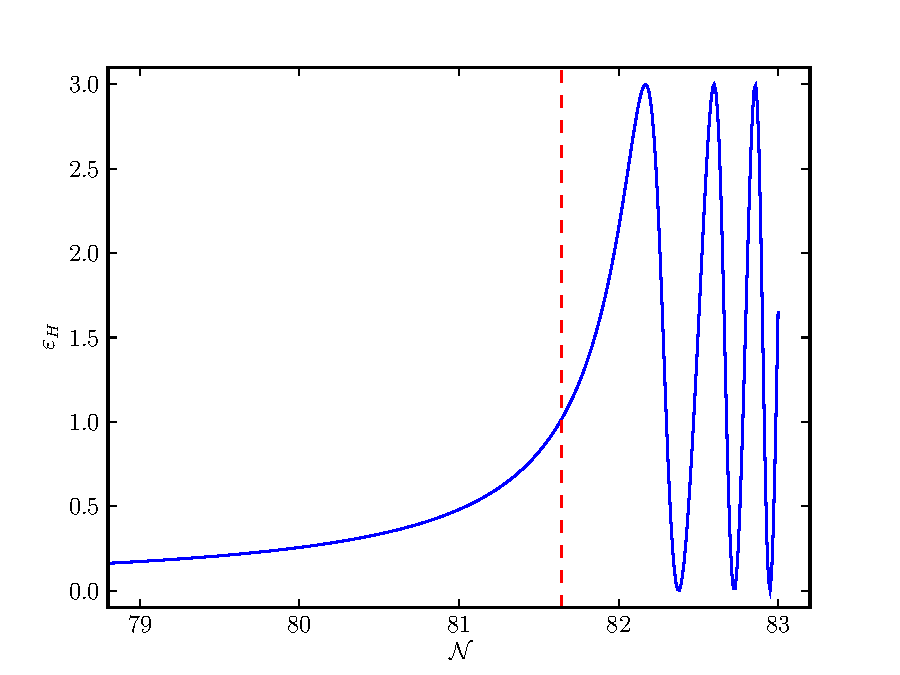
\includegraphics[scale=0.8]{./numerical/graphs/bgepsilon}
 \caption{The end of inflation is determined by calculating when
   $\varepsilon_H=-\dot{H}/H=1$ (red dashed line). Along the $x$-axis,
   $n$ is the number of e-foldings from the start of the
   simulation.}
\label{fig:eps}
\end{figure}

The system of ordinary differential equations for the first order
perturbations from \eq{eq:fontime} is calculated using a standard
Runge-Kutta method. A fixed time step method is used in order to
simplify the construction of the  second order source term and because
\emph{a priori} it is not known which time steps would be required at
second order if an adaptive time step system were used. The first
order equations are separable in terms of $k$ and so it is
straightforward to run multiple instances of the system and collate
the results at the end. However, as will be discussed below, the first
order calculation is not computationally expensive in comparison with
the other stages and takes of the order of a few minutes for around
$8000$ time steps and $1025$ $k$ modes.


Once the first order system has been solved 
the source term for the second order system must be calculated. As the
real space equation for the source involves terms quadratic in the
first order perturbation it is necessary to perform a convolution in
Fourier space, as shown in \eq{eq:KG2-fourier-sr-aterms}.  Transforming
back into real space was not considered due to the presence of both
gradient operators and their inverses. Here the slow roll version of
the source term integrand has been used, but the method can equally be
applied to the full equation. This stage is the most computationally
intensive and can be run in parallel as each time step is independent
of the others. The nature of the convolution integral and the
dependence of the first order perturbation on the absolute value of
its arguments requires that twice as many $k$ modes are calculated at
first order than are desired at second order as explained above.  As
the first order calculation is computationally cheaper than the source
term integration, this does not significantly lower the possible
resolution in $k$-space, which is still limited by the source term
computation time.  Once the integrand is determined it is fed into a
Romberg integration scheme. As for $\theta$  which was
discretised by $N_\theta$ points in \eq{eq:AtoD-num}, this requires that the
number of $k$ modes is
%
\begin{equation}
\label{eq:nk-constraint-num}
N_k=2^l + 1\,,
\end{equation}
%
for some\footnotemark $l\in\mathbb{N}$. 
\footnotetext{The number of discretised $k$ modes $N_k$ does not need to be equal to
  $N_\theta$.}
This requirement can be lifted by opting for a less
accurate and somewhat slower standard quadrature routine.


The second order system is finally run with the source term and other
necessary data being read as required from the memory or disk. The
Runge-Kutta method calculates half time steps for each required point,
for example if $y(x_n)$ is known and $y(x_{n+1})=y(x_n+h)$ is required
(for step size $h$), the method will calculate the derivatives of $y$
at $y(x_n), y(x_n +h/2)$ and $y(x_n + h)$. As we need to specify the
source term at every calculated timestep, the requested timestep for
the second order method must be twice that used at first order.  This decreases the
accuracy of the method but does not require the use
of splines and interpolation techniques to determine background and
1st order variables between time steps.


The second order system is similar in run time to the first order 
system but the
source integration is more complex, involving the
integration of $N_k^2\times N_\theta$ values at
each time step.
Although a large amount of data is produced at each step at this
stage for 
each of the wavenumbers $k$, only the integrated result is stored to be used
in the second order run.
Results for each stage are stored in the open HDF5 standard which can deal
efficiently with large
files and is very portable, allowing data analysis independent of the
Python/Numpy programming environment.
We intend to release the program under a suitable license once the code has
matured and some of the improvements discussed in Section \ref{sec:disc-num} have
been implemented.


%%%%%%%%%%%%%%%%%%%%%%%%%
\subsection{Code Tests}
\label{sec:codetests}
%%%%%%%%%%%%%%%%%%%%%%%%%


We have tested the numerical code in a variety of controlled
circumstances in order to quantify the effect of different choices of
parameters. In particular it is important to know whether the values
picked for $N_\theta$, the number of discretised $\theta$s, $\Delta k$, the size of the
spacing of the discretised $k$ modes, and the range of
$k$ values significantly impacts on the results. The ODE solving parts
of the code are straightforward and follow standard algorithms.


As mentioned above the WMAP results \cite{Komatsu:2008hk} use
observations in the range $k\in [0.92 \e{-60}, 3.1 \times
  10^{-58}]\Mpl = [3.5\e{-4}, 0.12] M_{\mathrm{pc}}^{-1}$. We will
consider three different $k$ ranges both in our results and the tests
of the code\footnotemark:
%
\begin{eqnarray}
\label{eq:Krangedefns}
K_1 &=& \left[1.9\e{-5}, 0.039\right]\Mpc^{-1}\,,\quad \Delta k = 3.8\e{-5}\Mpc^{-1}
\,,\nonumber\\
K_2 &=& \left[5.71\e{-5}, 0.12\right]\Mpc^{-1}\,, \quad \Delta k = 1.2\e{-4}\Mpc^{-1}\,,
\nonumber\\ 
K_3 &=& \left[0.52\e{-5}, 0.39\right]\Mpc^{-1}\,, \quad \Delta k = 3.8\e{-4}\Mpc^{-1} \,.
\end{eqnarray}
% 
\footnotetext{The $k$ ranges in $\Mpl$ are:
\begin{eqnarray*}
\label{eq:Krangedefns-mpl}
K_1 &=& \left[0.5\e{-61}, 1.0245\e{-58}\right]\Mpl\,,\quad \Delta k = 1\e{-61}\Mpl \nonumber\\
K_2 &=& \left[1.5\times 10^{-61}, 3.0735\e{-58}\right]\Mpl\,, \quad \Delta k = 3\e{-61}\Mpl
\nonumber\\ 
K_3 &=& \left[0.25\e{-60}, 1.02425\e{-57}\right]\Mpl\,, \quad \Delta k = 1\e{-60}\Mpl \,.
\end{eqnarray*}
}
% 
The first, $K_1$, has a very fine resolution but covers only a small portion of the WMAP range. 
The next, $K_2$, is closest to the WMAP range with a still quite fine resolution.  The final
range, $K_3$, has a larger $k$ mode step size $\Delta k = 1\e{-60}\Mpl = 3.8\e{-4}\Mpc^{-1}$ and
covers a greater range than the others, extending to much smaller scales than WMAP can observe.

\begin{figure}
% 
 \subfigure[The relative error for different $N_\theta$, the number of discretised $\theta$s,
 keeping the other
parameters fixed and using the $K_3$ range. The upper blue line ($N_\theta=129$)
and middle green line
 ($N_\theta=257$) have relative errors at least an order of magnitude larger than the lower red
line
($N_\theta=513$).]{
 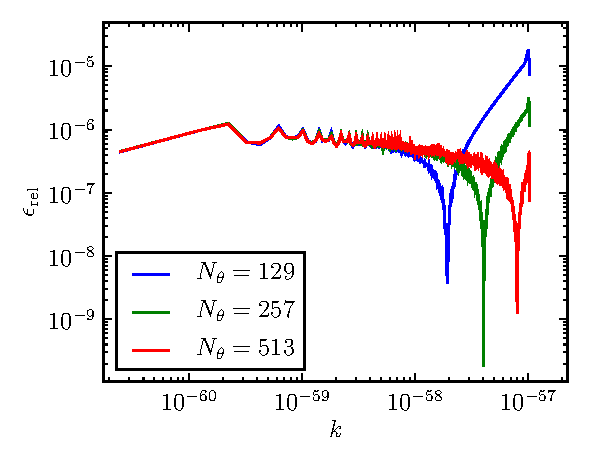
\includegraphics[scale=0.8]{numerical/graphs/err-nthetas-small.pdf}
 \label{fig:err-nthetas}
}
% 
\subfigure[The relative error for the 3 different $k$ ranges $K1$, $K2$,
$K3$ (starting from the left). The parameter $\Delta k$
is set equal to $1\e{-61}\Mpl, 3\e{-61}\Mpl, 1\e{-60}\Mpl$ respectively.]{
 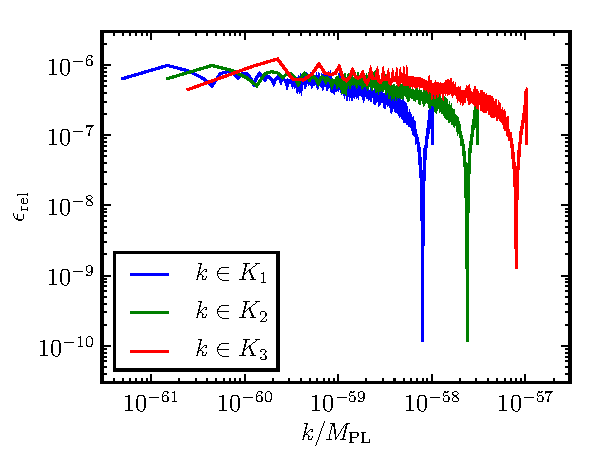
\includegraphics[scale=0.8]{numerical/graphs/err-kranges-small.pdf}
 \label{fig:err-kranges}
}
% 
\caption{Comparison of relative errors for different $N_\theta$ and $k$ ranges.}
\label{fig:err-comparison}
\end{figure}

The main new addition in the code is the calculation of the
convolution of the perturbations for the source term
\eq{eq:KG2-source-ntime}. In particular the first of the $\theta$ dependent terms in
\eq{eq:AtoD-num}, $A$,
can be convolved analytically for certain smooth $\dvp1(k)$s. 
 We take $\dvp1(k)$ to be similar in form to the initial conditions
(\ref{eq:foics}), for example $\dvp1(k)\propto 1/\sqrt{k}$ with proportionality constant
$\alpha$.
If $I_A$ denotes the convolution of the $A$ term:
% 
\begin{equation}
 I_A (k) = 2\pi \int_{\kmin}^{\kmax} q^2 \dvp1(q) A(k, q) dq \,,
\end{equation}
% 
then putting in $\dvp1(k) = \alpha/\sqrt{k}$ gives
% 
\begin{equation}
 I_A(k) = 2\pi \alpha^2 \int_{\kmin}^{\kmax} dq\, q^{\frac{3}{2}}
\int_{0}^{\pi} d\theta\, (k^2 + q^2 -2k q \cos{\theta})^{-4} \sin{\theta}\,. 
\end{equation}
% 
This has the analytic solution
% 
\begin{eqnarray}
\label{eq:err-analytic-num}
 A(k) &=& \frac{\pi}{18}\frac{\alpha^2}{k} \left\{ 
3k^3\left[\log\left(2\sqrt{k}\right) - \frac{\pi}{2}  + 
\arctan\left(\sqrt{\frac{\kmin}{k-\kmin}}\right) 
 + \log\left(2\left(\sqrt{\kmin} + \sqrt{\kmin + k}\right)\right) \right.\right. \nonumber \\
&& \left. -\, \log\left(2\left(\sqrt{\kmax} + \sqrt{\kmax + k}\right)\right) 
  - \log\left(2\left(\sqrt{\kmax} + \sqrt{\kmax - k}\right)\right) \right]  \nonumber \\
&& +\, \sqrt{\kmax}\left[\sqrt{\kmax -k} \left(-3k^2 + 14k\kmax - 8\kmax^2\right)  
 + \sqrt{\kmax +k} \left(3k^2 + 14k\kmax + 8\kmax^2\right)\right] \nonumber \\ 
&& \left. -\, \sqrt{\kmin}\left[\sqrt{k -\kmin} \left(3k^2 - 14k\kmax + 8\kmax^2\right) 
 - \sqrt{k +\kmin} \left(3k^2 + 14k\kmax + 8\kmax^2\right)\right] \right\} \,.
\end{eqnarray}
%
We have tested our code against this analytic solution for various
combinations of $k$ ranges and $N_\theta$. The relative error
%
\begin{equation}
 \epsilon_\mathrm{rel} = \frac{|\mathrm{analytic}- \mathrm{calculated} |}{|\mathrm{analytic}|}
\end{equation}
%
is small for all the tested cases but certain combinations of
parameters turned out to be better than others. The relative error of
all the following results is not affected by the choice of $\alpha$ so
we will keep it constant throughout.

\begin{figure}
 \centering
 \includegraphics[scale=0.8]{numerical/graphs/err-deltak4.pdf}
 \caption{The relative error in convolution term $A$ for different values of $\Delta k$.
The other parameters are fixed: $\kmin=1\times10^{-60}\Mpl, N_k = 1025$ and $N_\theta=513$. The
upper 
blue line ($\Delta k=1\e{-61}\Mpl$ and middle green line ($\Delta k=3\e{-61}\Mpl$) have relative
errors at
least an order of magnitude larger than the lower red line ($\Delta k=1\e{-60}\Mpl$).}
 \label{fig:err-deltaks}
\end{figure}


We first tested the effect of changing $N_\theta$, the number of
samples of the $\theta$ range $[0,\pi]$.  Figure~\ref{fig:err-nthetas}
plots these results for the $k$ range $K_3$ with $\Delta k =
1\e{-60}\Mpl$. Only three values of $N_\theta$ are shown for clarity. It
can be seen that increasing $N_\theta$ decreases the relative error (for the convolution
term at least) when the other parameters are kept constant, as one
might expect.


As mentioned above the choice of $k$ range is especially important as
the convolution of the terms depends heavily on the minimum and
maximum values of this range. Indeed this is clear from the analytic
solution in \eq{eq:err-analytic-num}. Figure~\ref{fig:err-kranges}
shows the difference in relative error for the three different $k$
ranges described above with 
% Mpc values 
$\Delta k= 3.8\e{-5}, 1.2\e{-4}$ and $3.8\e{-4}\Mpc^{-1}$
% Mpl values
($\Delta k= 1\e{-61}, 3\e{-61},1\e{-60}\Mpl$)
respectively. The accuracy is similar in all three cases.


Another important check is whether the resolution of the $k$ range is
fine enough. Varying $\Delta k$ can not be done in isolation of
course, if the constraint for $N_k$, \eq{eq:nk-constraint-num},
is to
be met. For this test the end of the $k$ range changed with $\Delta k$
but the other parameters were kept fixed as $\kmin=1\e{-60}\Mpl=3.8\e{-4}\Mpc^{-1},
N_k = 1025$ and $N_\theta=513$. Figure~\ref{fig:err-deltaks} plots
these results again for only three indicative values.  For $\Delta
k<\kmin$, here the upper two lines, there is a marked degradation in
the accuracy of the method. This is understandable as many
interpolations of multiples of $\Delta k$ below $\kmin$ will be set to
$0$. Once $\Delta k$ is greater than $\kmin$ the relative error is
very similar for higher values (not shown in the figure).


\begin{figure}
 \centering
 \includegraphics[scale=0.8]{numerical/graphs/err-deltak-kmin.pdf}
 % err-deltak-kmin.pdf: 432x324 pixel, 72dpi, 15.24x11.43 cm, bb=
 \caption{The relative error of the convolution term for three different values of $\Delta k$. In
contrast to Figure~\ref{fig:err-deltaks} $\kmin=1\e{-61}\Mpl=3.8\e{-5}\Mpc^{-1} \le \Delta k$ for
each.}
 \label{fig:err-deltak-kmin}
\end{figure}


It should be noted that these tests show the relative errors in the
computation of the $A$ convolution term, the most straightforward term in \eq{eq:AtoD-num}, only and
do not
represent
errors for the full calculation. However, they show that at least for
the pure convolution term the accuracy is good compared with the
analytic results. Equation (\ref{eq:err-analytic-num}) gives some indication of
the difficulty involved in finding an analytic solution for the other
terms, although this is a goal for future work. Having described the
implementation and accuracy of the numerical system we will outline
our results in the next section.
 
% 
% 
% 
% % % % % % % % % % % % % % % % % % % % % % % % % % % % % % % % 
% =========================================================== %
% % % % % % % % % % % % % % % % % % % % % % % % % % % % % % % %
\section{Results}
\label{sec:results}
% % % % % % % % % % % % % % % % % % % % % % % % % % % % % % % % 
% =========================================================== %
% % % % % % % % % % % % % % % % % % % % % % % % % % % % % % % %


The main result of this paper is the demonstration of a numerical solution to
the closed Klein-Gordon equation of motion for second order scalar field
perturbations as described in \eq{eq:KG2-fourier-sr-num}. This includes the slow
roll approximation of the source term for second order perturbations, but we have not used a slow
roll version of the evolution equations for the background or first order
perturbations. 

As a proof of concept we have tested the system with two standard potentials,
$\msqphisq$ and $\lambdaphifour$ and computed results across three
different $k$ ranges. As expected, considering the use of a single slowly
rolling field, the second order perturbation we have calculated is extremely
small in comparison with the first order term. However there are already
differences apparent between the two potentials which will be outlined below.
We have calibrated the parameters $m$ and $\lambda$ of the potentials using the
WMAP 5 normalisation at $\kwmap=0.002 \Mpc^{-1} = 5.25 \e{-60}\Mpl$
\cite{Komatsu:2008hk}.
We have outlined in \eq{eq:Krangedefns} the three $k$ ranges that we will use,
% 
\begin{eqnarray*}
K_1 &=& \left[1.9\e{-5}, 0.039\right]\Mpc^{-1}\,,\quad \Delta k = 3.8\e{-5}\Mpc^{-1} \nonumber\\
K_2 &=& \left[5.71\e{-5}, 0.12\right]\Mpc^{-1}\,, \quad \Delta k = 1.2\e{-4}\Mpc^{-1}
\nonumber\\ 
K_3 &=& \left[0.52\e{-5}, 0.39\right]\Mpc^{-1}\,, \quad \Delta k = 3.8\e{-4}\Mpc^{-1} \,.
\end{eqnarray*}
Many of the results will be quoted for $\kwmap$ which lies in all three of these ranges.

Given that the first order perturbations for the chosen potentials give an
almost scale invariant power spectrum with no running, it is no surprise that
the results from the three different $k$ ranges are very similar. The second
order source term is somewhat dependent on the lower bound of $k$ (upper bound
on size). This is expected and in the scale invariant case a log divergence can
be shown to exist \cite{Lyth:2007jh}. We have implemented an arbitrary sharp cutoff at $\kmin$
below
which 
$\dvp1$ is taken to be zero. As mentioned above there is some evidence to suggest that a 
similar cutoff is supported by the WMAP data \cite{Sinha:2005mn,Kim:2009pf}. 
% 
% % % % % % % % % % % % % % % % % % % % % % % % % % % % % % % % % % 

At first order our solutions agree with previous work
\cite{Salopek:1988qh,Martin:2006rs,Ringeval:2007am}, with oscillations
being damped until horizon crossing (when $k=aH$) after which the
curvature perturbation becomes conserved. Figure~\ref{fig:dp1} shows
the real and imaginary parts of the first order perturbations from
when the initial conditions are set at $k/aH=50$ to just after horizon
crossing. The x-axis for most of the following figures shows the
number of e-foldings left until the end of inflation instead of the
internally used time variable $n$.
%
% 
\begin{figure}
 \centering
 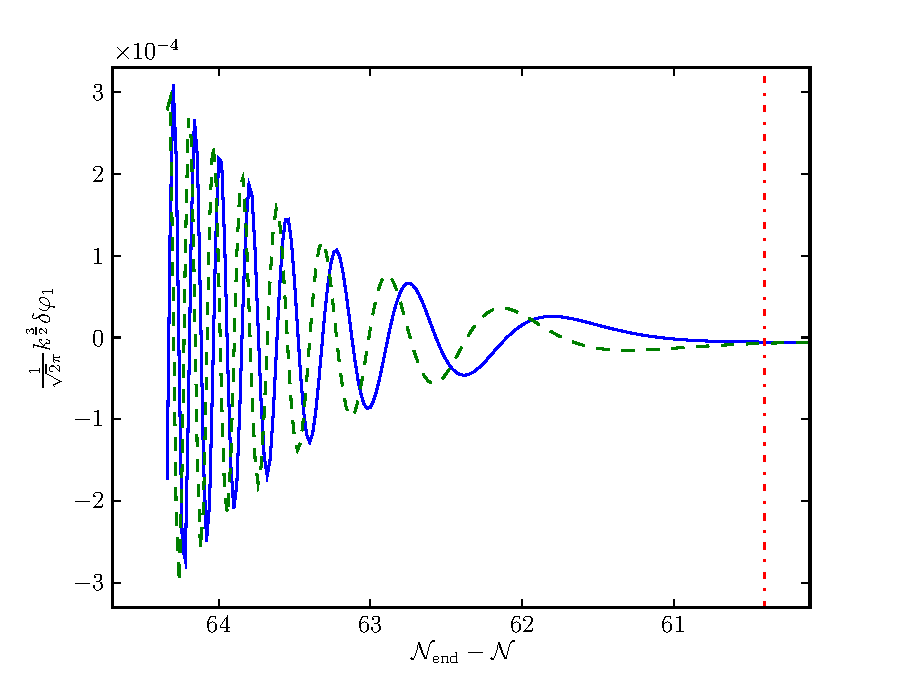
\includegraphics[scale=0.8]{numerical/graphs/dp1_kwmap}
 \caption{The first order perturbation $\dvp1$ rescaled by
$k^{3/2}/(\sqrt{2}\pi)$ from the beginning of the simulation until around
horizon crossing (red dot-dashed line). The real (blue) and imaginary (green
dashed) perturbations are shown for $\kwmap$.}
\label{fig:dp1}
\end{figure}
% 
% % % % % % % % % % % % % % % % % % % % % % % % % % % % % % % % % % % 



In Figure~\ref{fig:dp2realimag} we show the evolution of the second
order perturbations for wavenumber $\kwmap$. As mentioned above the
overall amplitude of the second order perturbations is many orders of
magnitude smaller than the first order ones. In Figures~\ref{fig:dp1}
and \ref{fig:dp2realimag} the field values have been rescaled by
$k^{3/2}/(\sqrt{2}\pi)$ to allow a better appreciation of the
magnitude of the resulting power spectra.
% 
\begin{figure}
 \centering
 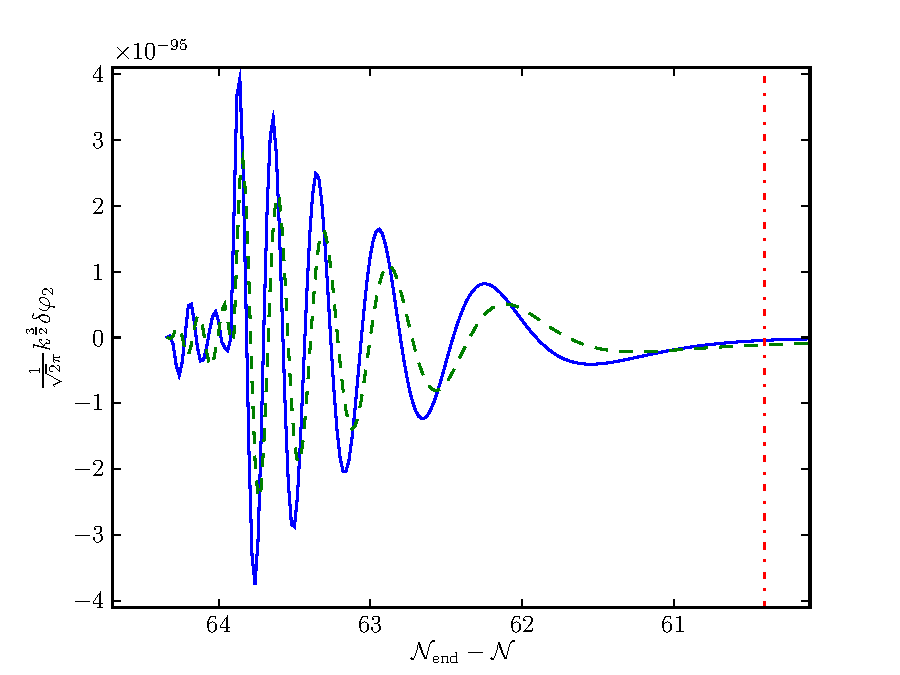
\includegraphics[scale=0.8]{numerical/graphs/dp2_kwmap}
 \caption{The real (blue line) and imaginary (green dashed) components of the second order
perturbation $\dvp2(\kwmap)$ from the beginning of the simulation until around the time
of horizon exit (red dot-dashed line).}
\label{fig:dp2realimag}
\end{figure}
% 
% % % % % % % % % % % % % % % % % % % % % % % % % % % % % % % % % % % 



The source term $S(\kvi)$ is calculated at each time step using the
results of the first order and background runs. This term drives the
production of second order perturbations as shown in
\eqs{eq:KG2-fourier-sr-num} and
(\ref{eq:KG2-fourier-sr-ntime}). Figure~\ref{fig:src-full} shows the
absolute magnitude of the source term for a single $k$ mode, $\kwmap$,
for all time steps calculated.
% 
\begin{figure}
\subfigure[Absolute magnitude of the source term.]{
 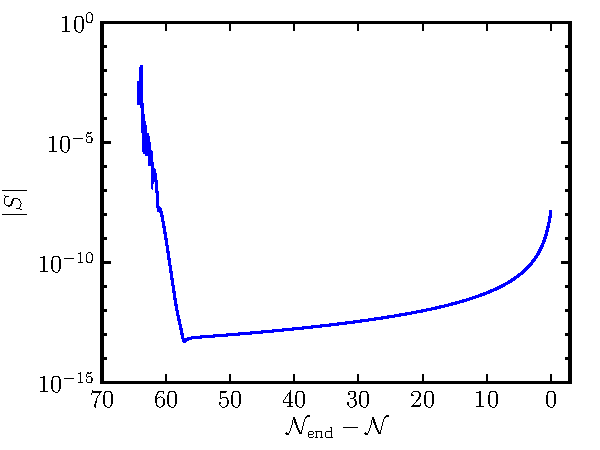
\includegraphics[scale=0.8]{numerical/graphs/src-kwmap-small}
\label{fig:src-full}
}
% 
\subfigure[Power spectrum of scalar perturbations $\mathcal{P}_{\delta\varphi} =
\frac{k^3}{2\pi^2}
|\delta\varphi|^2$.]{
 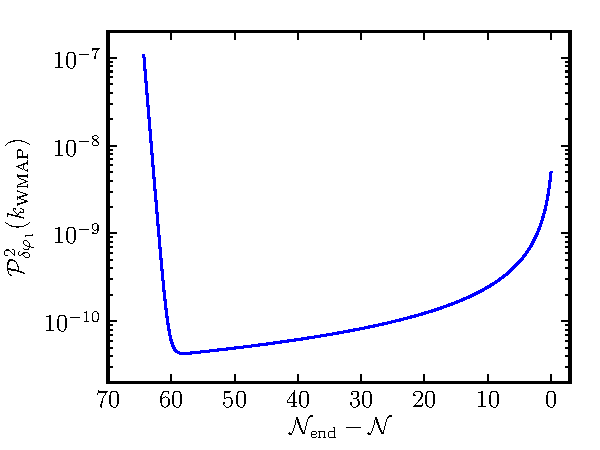
\includegraphics[scale=0.8]{numerical/graphs/Pphi-kwmap-nohoriz-small}
\label{fig:Pphi-kwmap}
}
\caption{Source term and power spectrum for the WMAP pivot scale $\kwmap$.}
\end{figure}
% 
Figure~\ref{fig:src-kwmap-3ranges} shows how the source term changes
with the choice of $k$ range.  After horizon crossing the source terms
are approximately equal. Before horizon crossing however there is a
strict hierarchy with the smaller $k$ ranges, $K_1$ and $K_2$, leading to smaller source
contributions.  As stated in Section \ref{sec:codetests}, $\Delta k$
should be at least as large as $\kmin$ in order to reduce the error to
a minimum.
% 
\begin{figure}
 \subfigure[Comparison of the source term for $\kwmap$ over three
different
ranges with different $\Delta k$s as specified in \eq{eq:Krangedefns}.]{
 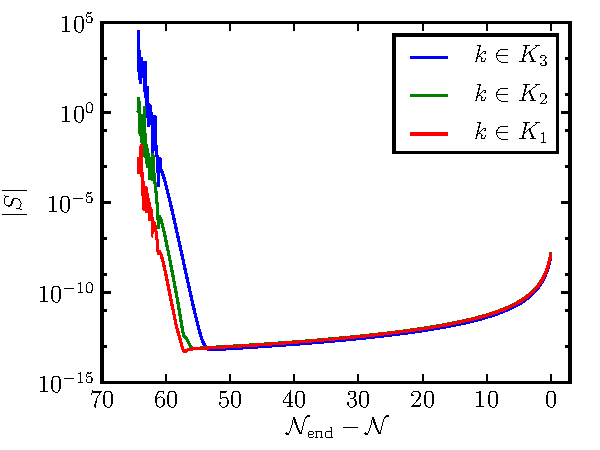
\includegraphics[scale=0.8]{numerical/graphs/src-kwmap-3ranges-small}
 \label{fig:src-kwmap-3ranges}
}
% 
\subfigure[The source term for three different $k$ values including the WMAP pivot scale. As $k$
gets larger (scale gets smaller) the source term becomes smaller.]{
 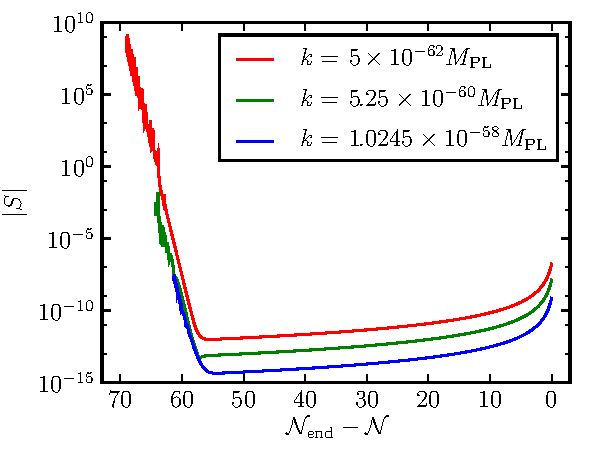
\includegraphics[scale=0.8]{numerical/graphs/src-3ks-small}
\label{fig:src-3ks}
}
\caption{Two different comparisons of the source term $S$.}
\label{fig:src-comparisons}
\end{figure}
% 
% 



The source term is large at early times, and closely follows the form
of the spectrum of the first order perturbations as can be seen from
Figure~\ref{fig:Pphi-kwmap}.
%
It is useful to compare the magnitude of the source term with the
other terms in the second order evolution equation
(\ref{eq:KG2-fourier-sr-ntime}). If we let $T$ denote the other terms,
%
\begin{equation}
\label{eq:Tdefn}
 T(\kvi) = \left(3 + \frac{\dot{H}}{H}\right)
\dot{\dvp2}(\kvi)+ \left(\frac{k}{aH}\right)^2\dvp2(\kvi)
+\left(\frac{\Upp}{H^2}-{24 \pi G}(\dot{\vp_{0}})^2\right)
\dvp2(\kvi) \,,
\end{equation}
%
then Figure~\ref{fig:src-vs-others} shows the absolute magnitude of
both $S$ and $T$.  It is clear that the source term is of comparable
magnitude only early in the simulation.  Figure~\ref{fig:s-over-t-3ks}
shows a comparison of $|S|/|T|$ for three different $k$ values. The larger the $k$ mode the closer
in amplitude $S$ is to the rest of the terms in the ODE.
A priori it is not known
where $S$ will be large for a particular chosen potential and mode but
once determined it could be possible to significantly reduce the time required
for the simulation by only calculating $S$ in the regions where it is
important.
%
\begin{figure}
% 
\subfigure[The source term (lower blue line) is compared with the $T$ term (upper green
line) as defined in the text for $\kwmap$. The source term is of comparable magnitude at the
beginning of the simulation. ]{
 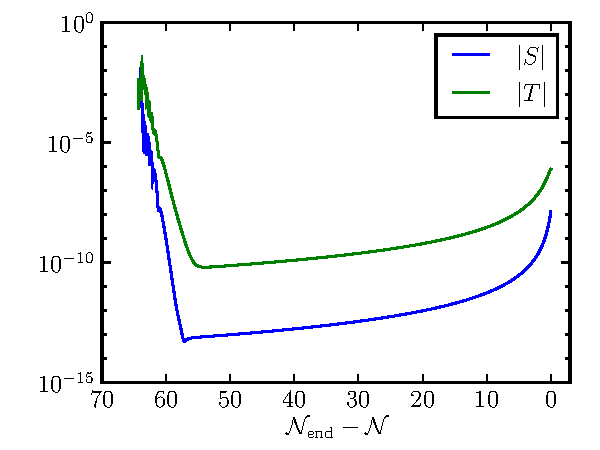
\includegraphics[scale=0.8]{numerical/graphs/src-vs-t-kwmap-small.pdf}
 \label{fig:src-vs-others}
}
% 
 \subfigure[The quotient of $S$ and $T$ terms for three different $k$ values including
the WMAP pivot scale. Depending on $k$ the source term only dominates at early stages or is
important throughout the evolution.]{
 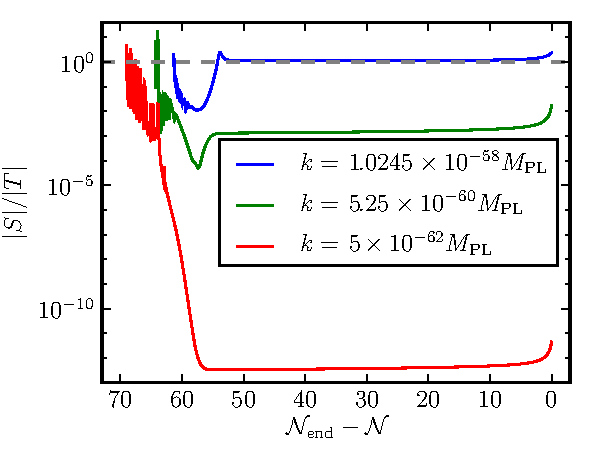
\includegraphics[scale=0.8]{numerical/graphs/s-over-t-3ks-small}
 \label{fig:s-over-t-3ks}
}
% 
\caption{Source term $S$ compared with $T$.} 
\label{fig:src-3ks-and-over-t}
\end{figure}
% 
% 
% % % % % % % % % % % % % % % % % % % % % % % % % % % % % % % % % % 


All the results quoted so far are for
the $\msqphisq$ model. We have also tested the $\lambdaphifour$ model and compared it to
$\msqphisq$. Figure~\ref{fig:src-mvl-main} compares the models for $\kwmap$.
Figure~\ref{fig:src-mvl-zoom} shows how the source term for the $\lambdaphifour$ model is larger
than the one for $\msqphisq$ to begin, but crosses over after a few e-foldings. After horizon
crossing the $\lambdaphifour$ source term is again larger. As the results at first order for both
models are so similar it is to be expected that the second order perturbations would be closely
related. 
% 
\begin{figure}
 \subfigure[The $\lambdaphifour$ model (green dashed line) initially has a larger source term but
becomes
smaller than the $\msqphisq$ model as evolution continues. After horizon crossing
the $\lambdaphifour$ term is slightly larger.]{
 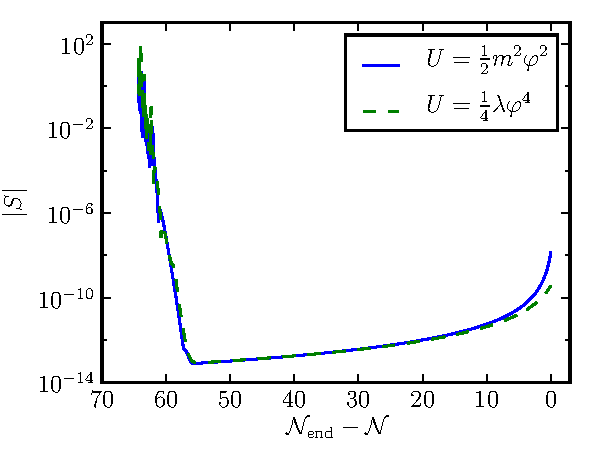
\includegraphics[scale=0.8]{numerical/graphs/src-mvl-small}
 \label{fig:src-mvl}
}
% 
\subfigure[The crossover between the models at the early stages of the simulation, before horizon 
crossing.]{
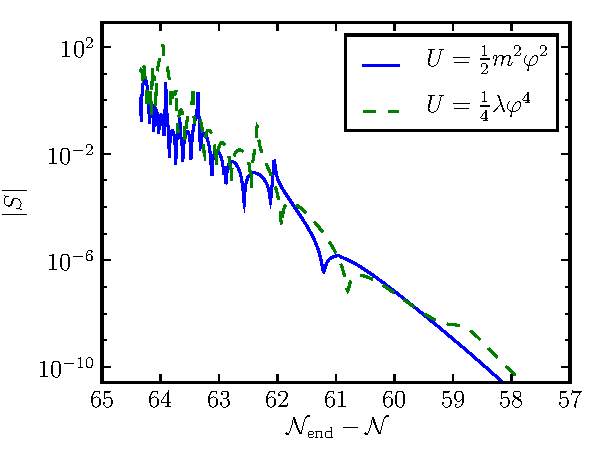
\includegraphics[scale=0.8]{numerical/graphs/src-mvl-zoom-small}
\label{fig:src-mvl-zoom}
}
\caption{A comparison of the source term for the $\msqphisq$ and
$\lambdaphifour$ models.}
\label{fig:src-mvl-main}
\end{figure}
% 
% % % % % % % % % % % % % % % % % % % % % % % % % % % % % % % % % % %

In Figure~\ref{fig:src-kinit} the value of $|S|$ at the start of the evolution of $\dvp2$ for
each $k$ mode is shown. The magnitude of the source term is much smaller for larger $k$s (smaller
scales). 
Because the smaller $k$s begin their evolution earlier the relative difference in $|S|$ is not as
pronounced when measured at a single timestep (see for example Figure~\ref{fig:src-3ks}).
It should also be remembered that the magnitude of other terms in the second order ODE is
small for larger $k$s as shown by the ratio $|S|/|T|$ in Figure~\ref{fig:src-3ks-and-over-t}
where $T$ is defined above in \eq{eq:Tdefn}.
\begin{figure}
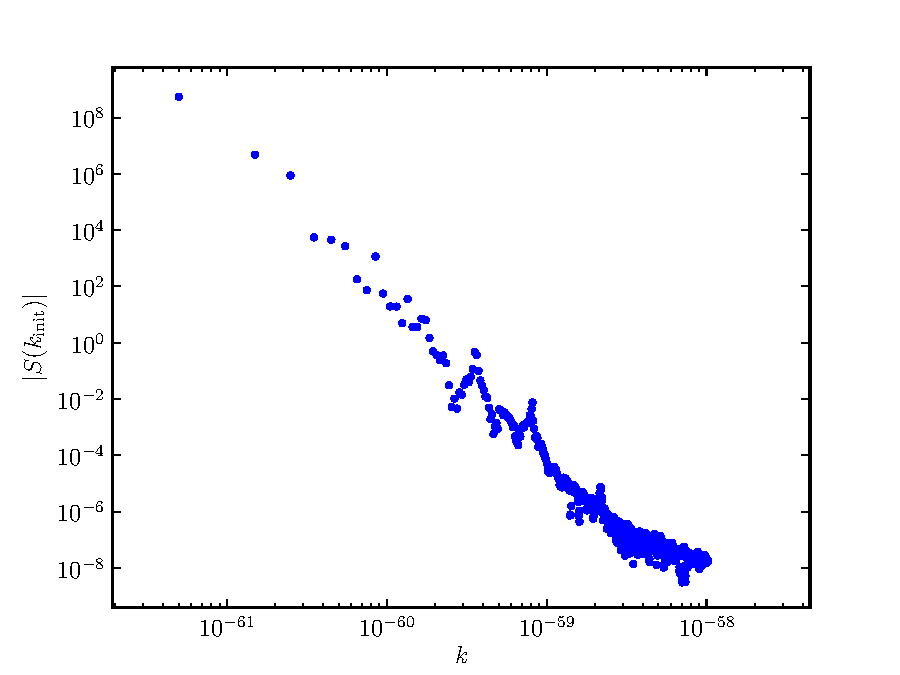
\includegraphics[scale=0.8]{numerical/graphs/src_kinit_log}
 \caption{The absolute magnitude of the source term at the initial start time for each $k$ when
$k = aH \times 50$ deep inside the horizon. The results are for the range $K_1=\left[ 1.9\e{-5},
0.039 \right] \Mpc^{-1}= \left[0.5\e{-61}, 1.0245\e{-58}\right]\Mpl$.}
\label{fig:src-kinit}
\end{figure}
% 

The source term for all $k$s can also be compared for different timesteps. In
Figure~\ref{fig:src-3ns} the upper blue line shows $|S(k)|$ around 69 e-foldings before the end of
inflation when $\dvp2$ has been initialised for only the very smallest $k$ modes. The middle green
line shows $|S|$ when all $\dvp2$ modes have been started. Finally the lower red line plots $|S|$
after all modes have exited the horizon, around 52 e-foldings before the end of inflation.
\begin{figure}
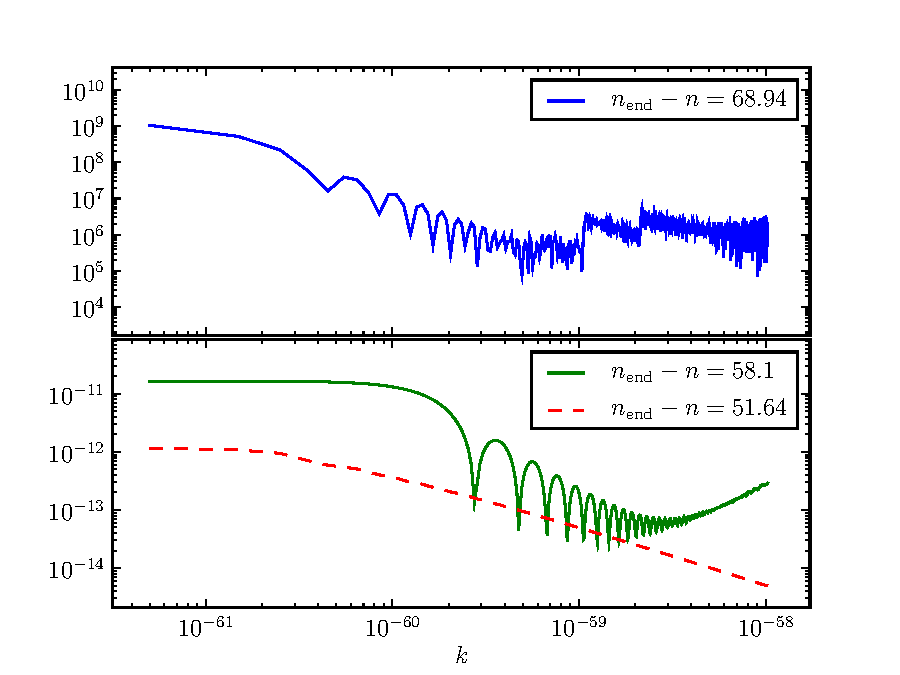
\includegraphics[scale=0.8]{numerical/graphs/src_3ns}
\caption{The absolute magnitude of the source term for all $ks$ in the range at three different
timesteps: the upper blue line when only the largest modes have been initialised; the middle green
line when all modes have been initialised; and the lower red dashed line when all modes have
exited the horizon. The $k$ range shown here is $K_1=\left[ 1.9\e{-5}, 0.039 \right] \Mpc^{-1}= 
 \left[0.5\e{-61}, 1.0245\e{-58}\right]\Mpl$.}
\label{fig:src-3ns}
\end{figure}
% 
% % % % % % % % % % % % % % % % % % % % % % % % % % % % % % % % 

% 
% 
% 
% % % % % % % % % % % % % % % % % % % % % % % % % % % % % % % % 
% =========================================================== %
% % % % % % % % % % % % % % % % % % % % % % % % % % % % % % % %
\section{Discussion and conclusion}
\label{sec:disc-num}
% % % % % % % % % % % % % % % % % % % % % % % % % % % % % % % % 
% =========================================================== %
% % % % % % % % % % % % % % % % % % % % % % % % % % % % % % % %

In this paper we have described the numerical solution of the
evolution equations for second order scalar perturbations, using the
closed form of the Klein-Gordon equation, \eq{eq:KG2-fourier-sr-num}. We
demonstrate that direct calculation of field perturbations beyond
first order using perturbation theory is readily achievable, though
not trivial.

For this first demonstration we have limited ourselves to considering
the slow roll source term in \eq{eq:KG2-fourier-sr-num} but without imposing
slow roll on the evolution terms of the ODEs. We have investigated two
standard potentials, $\frac{1}{2}m^2\phi^2$ and
$\frac{1}{4}\lambda\phi^4$, to demonstrate the capabilities of the
system. The singularity at $k=0$ which arises as larger and larger
scales are considered is avoided by implementing a cutoff at small
wavenumbers below $\kmin$. This is a pragmatic choice necessary for
the calculation, but as mentioned above there is some evidence that
such a cutoff might also explain lack of power at large scales in the
WMAP data \cite{spergel, Sinha:2005mn, Kim:2009pf}. It is also necessary to
pick a maximum $k$ value, and this choice is dictated by computational
resources and with reference to observationally relevant scales. In
this paper we have used $k$ ranges which are comparable with the
scales observed by WMAP. By comparing the analytical results of the
convolution integral with the numerical calculation, we have chosen
values of the parameters $N_\theta, N_k$ and $\Delta k$ which minimise
the numerical error. The convolution scheme that we have implemented
works best when $\Delta k>\kmin$.


We have shown explicitly that the second order calculations for our chosen
potentials are obtainable once the cut-off for $\kmin$ is
implemented. As expected for these unexceptional potentials in the slowly
rolling regime the magnitude of second order perturbations is extremely
suppressed in comparison with the first order amplitude. We have shown the
evolution of the source term equation during the inflationary regime can be
readily calculated.


There are many possible next steps to improve the program outlined in
Section \ref{sec:numerics}. Chief amongst these is to implement the
full source term equation (\ref{eq:KG2-source-ntime}). Although clearly
more complicated than the slow roll case in \eq{eq:KG2-fourier-sr-ntime}
only two more $\theta$ dependent terms need to be added to $A$--$D$ in
\eq{eq:AtoD-num}.  For the two test models we have used in this paper, which
are both slowly rolling during inflation, it is not expected that
using the full source equation would result in an appreciably
different outcome until the end of the inflationary phase. Though once
the field has stopped to roll slowly, new observable features might
arise as is indeed the case at first order. 


Beyond this the next likely step is to implement a multi-field version of the
system. This would allow the investigation of models that inherently
produce large second order perturbations. In Ref.~\cite{Malik:2006ir} the
Klein-Gordon equation is given for multiple fields and upgrading the
simulation to use these equations is a
straight-forward if lengthy process.  


The performance of the numerical simulation could also be improved by
analysing the most time consuming processes and investigating what
optimisations could be implemented. As we have discussed above we have
set $N_k=1025$ for our test runs. This provides good coverage of the
WMAP $k$ range but it is not clear whether it sufficiently
approximates the integral to infinity for the source term.  Currently
we are restricted in our choice of $N_k$ by logistical factors \ie the
running time and memory usage of the code. By optimising the routines
for both memory and speed it is hoped we can extend the maximum value
of $k$ to larger values.


By computing the perturbations to second order we have direct access
to the non-gaussianity of $\dvp{}$.  While useful for the toy models
discussed above (with $\fnl\simeq0$), when used to investigate models
with predictions of large non-linearity parameter $\fnl$ this technique
could yield greater insight into the formation and development of the
non-gaussian contributions by studying the contribution of the different
terms in the source term \eq{eq:KG2-source-ntime}.
%
It was shown recently that in order to calculate $\fnl$ instead of
using the standard method based on the Lagrangian formalism
\cite{Maldacena:2002vr}, one can instead use the field equations
\cite{Musso:2006pt,Seery:2008qj}. The method presented here will
therefore eventually allow a full numerical calculation of $\fnl$.


In summary, we have demonstrated that numerically solving the closed
Klein-Gordon equation for second order perturbations is possible. We
have used the slow roll version of the source term in this paper, but
hope to extend our work to use the full source soon. The two test
models we have used have been shown to have negligible second order
perturbations in line with analytic results. We have compared the
analytic and numerical solutions for the convolution term and found
them to be in good agreement.

%%%%%%%%%%%%%%%%%%%%%%%%%%%%
%\part*{}%Stuff at the end}
%%%%%%%%%%%%%%%%%%%%%%%%%%%%%
\chapter{Concluding summary}

% % % % % % % % % % % % % % % % % % % % % % % 
% theend.tex - Ian Huston
% $Id: theend.tex,v 1.17 2009/11/22 18:32:41 ith Exp $
% % % % % % % % % % % % % % % % % % % % % % 
% Redefine CVSRevision for this section
\renewcommand{\CVSrevision}%
{\version$Id: theend.tex,v 1.17 2009/11/22 18:32:41 ith Exp $}

% % % % % % % % % % % % % % % % % % % % % % % % % % % % % % % % 
% =========================================================== %
% % % % % % % % % % % % % % % % % % % % % % % % % % % % % % % %
\chapter{Conclusion and Discussion}
\label{ch:conclusions}
% % % % % % % % % % % % % % % % % % % % % % % % % % % % % % % % 
% =========================================================== %
% % % % % % % % % % % % % % % % % % % % % % % % % % % % % % % %

As the number of viable cosmological models increases, the need to constrain them becomes more
important. At the same time, the quantity and quality of observational data continues to improve.
There now exists the opportunity to go beyond linear statistical analyses
and confront the predictions of models with observational data from the non-linear
regime. In this thesis both analytic and numerical methods have been developed to
constrain inflationary models.

The framework used in this thesis is the Friedmann-Robertson-Walker universe,
reviewed in Chapter~\ref{ch:introduction}. During the accelerated expansion of the
inflationary period, quantum fluctuations seeded energy density variations, which in turn
gave rise to the diverse structure of the present universe. First order
cosmological perturbation theory
is necessary to describe the evolution of these fluctuations. The main observable
quantities can be calculated at horizon crossing by using the Bunch-Davies vacuum
initial conditions. The departure of the perturbations from a purely Gaussian random
field is parametrised by $\fnl$, which is described in two limits, local and
equilateral. 
In addition to canonical actions, we also introduced
non-canonical models, for which the speed of sound of the perturbations plays a
crucial role. When the sound speed is small, the amplitude of $\fnleq$ for these
models is large. 



% DBI
In Part~\ref{part:dbi}, analytic methods were developed to constrain
string theory inspired non-canonical inflationary models. The Dirac-Born-Infeld
scenario was
outlined in Chapter~\ref{ch:dbi-intro}. In this model, a D3-brane propagates in a
six-dimensional warped throat. The radial position of the brane from the tip of the
throat assumes the role of the inflaton field. The non-canonical nature of the DBI
action restricts the kinetic energy of this field no matter how steep the potential.
This allows an inflationary period of sufficient duration to occur.
This model was widely regarded as a very promising realisation of an inflationary
model in a string-theory context.

In \Rref{bmpaper}, Baumann and McAllister used the Lyth bound \cite{lyth} to limit
the tensor-scalar ratio. Their analysis was based on the conservative assumption that the brane
could
not propagate further than the full length of the throat. In Chapter~\ref{ch:dbi},
we showed that this bound can be tightened by applying it over the
portion of the throat through which the brane passes during the directly observable
stage of inflation. Restricting the field variation to be over these
approximately four e-foldings constrains $r$ to be less than $10^{-7}$ for standard
parameter values.

The most optimistic estimates of advances in experimental techniques and data
analysis, including foreground reduction, indicate that observations of $r>10^{-4}$
might be achievable in the future \cite{Baumann:2008aq,vpj}. Therefore, the new bound in
\eq{eq:upperbound} immediately rules out the observation of a tensor mode signal
from this model.

In addition to this, we also derived a lower bound on $r$ in \eq{eq:lowerbound}.
This depends on observable quantities, namely the scalar spectral index and the
equilateral non-gaussianity. Saturating the WMAP5 observational limit on $\fnleq$
and taking the best fit value for $n_s$, we found that the most conservative lower
limit is $r>0.005$. This is clearly incompatible with the previously derived upper
bound. Therefore, for standard parameter values, the D3-brane DBI scenario is not
viable. Numerical simulations by Peiris \etal in \Rref{Peiris:2007gz} have
demonstrated the lower bound, in the relativistic limit, using the
Hamiltonian flow approach.

The discovery of these incompatible bounds for DBI inflation has had a noticeable
impact on the research community, spurring interest in finding models which evade
these bounds. Many such models have been proposed with varying degrees of success. In
Section~\ref{sec:others-dbi} these were categorised according to whether they
featured single or multiple fields, and single or multiple branes. 

In Section~\ref{sec:relaxing-dbi}, a phenomenological approach was taken to easing
the upper bound on the tensor-scalar ratio. By considering a DBI-type action with unspecified field
functions,
$f_i$, we showed that the generalised lower and upper bounds can be consistent
if the product of $f_1$ and $f_2$ is sufficiently large on observable scales.


% Multi
More general actions, which relax the bounds on $r$, were derived in
Chapter~\ref{ch:multibrane}. 
We found a class of actions similar in form to that of the DBI model. 
However, instead of a square-root in the kinetic term, the index of the main term of these
actions depends on the constant of proportionality between $\Lambda$ and the sound
speed of inflaton fluctuations.
The upper bound on $r$ can be derived for these general actions and when the index
is below the critical value of $1/2$ (corresponding to the standard DBI scenario), this bound is
significantly relaxed.  
When new models are proposed in the future, our phenomenological derivation of this family of
actions will allow those models for which the bound on $r$ is less stringent to be easily
identified.

Once such model is the single field, coincident brane scenario of
Thomas \& Ward \cite{thomasward}. When $n$ D3-branes propagate in a throat, the
non-Abelian interactions between the branes result in major departures from the
single brane case. This is in contrast to the non-interacting branes model, in which
the total action is simply the sum of copies of the single brane action.

In the limit of a large number of branes being coincident, the effective action is
similar to $n$ times the single brane model, with the addition of a fuzzy potential
term. The bounds on $r$ can be somewhat relaxed when this potential is large,
but the model is still strongly constrained by current observations. For an $AdS_5$
throat, standard parameter choices limit the number of allowed branes to be
less than 150, at which point the assumption of arbitrarily large $n$ becomes
questionable.

More promising is the finite $n$ limit of the coincident brane model. The
non-Abelian nature of the interactions leads, in this case, to a recursive relation for
the $n$-brane action in terms of the $n=2$ one. In
Section~\ref{sec:finiten-multi} we showed that the action for finite $n$ is one of
the class of bound-evading actions described above. This identification is possible
because the last term of the recursive sum dominates in the relativistic limit. This
approximation is valid at least when $n<10$ and the backreaction of the multiple
branes is kept well under control for this range of $n$.

Although the bounds on $r$ are eased
for this model, we showed that observations strongly constrain the possibility of
an observable tensor signal being generated. If an observable tensor-scalar ratio is
considered to be $r>10^{-4}$ then only the two or three brane cases are capable of
producing such a signal. This bound on $n$ depends on the WMAP5 limit on $\fnleq$.
If, as expected, the observational limits on $\fnleq$ tighten considerably in the
future, the possibility of an observable tensor signal from the multi-coincident
brane model could be ruled out.

% Numerical
In Part~\ref{part:numerical} of this thesis, numerical methods were used to test inflationary
models up to second order in cosmological perturbation theory. 
% 
% 
The Klein-Gordon equation at second order was derived in \Rref{Malik:2006ir} for the
multi-field case. 
In Chapter~\ref{ch:perts}, second order gauge transformations were outlined
and the Klein-Gordon equation reproduced for a single scalar field model. In contrast
to the $\Delta \N$ approach, this equation is valid on all scales, both inside and
outside the horizon. 


In Fourier space, the second order Klein-Gordon equation \eqref{eq:SOKG-real-num} contains a
convolution term of the first order scalar field perturbation. For this first
demonstration of the numerical system, a slow roll approximation of the full
equation was used. 

Calculating the second order scalar field perturbations provides the possibility of
a unique insight into the generation and evolution of non-linear contributions to
the scalar curvature perturbation. The long term aim of this continuing project is
to analyse multi-field, non-slow roll models, in which non-Gaussian effects are
expected to play an important role.

One advantage of using the inflaton field equations is that we can directly
investigate the generation of the perturbations. Integrating the evolution
equation for a derived observable quantity would, instead, add a degree of
separation from the physical origins of the perturbation. Indeed, there is, as yet,
no known evolution equation for one of the main observable quantities, the comoving
curvature perturbation, at second order. 


As a step towards this goal, we described the implementation of a numerical
calculation of the single field, slow roll, second order equation in
Chapter~\ref{ch:numericalsystem}. The construction and evaluation of the convolved
source term in \eq{eq:KG2-src-sr-aterms} proved to be the most numerically complex
step required. 

To allow a numerical calculation, an energy scale cutoff must be implemented. We used
a sharp cutoff at small wavenumbers below which the perturbations were taken to be
identically zero. Another cutoff at small scales (or equivalently large wavenumbers) was dictated
by practical considerations of calculation size and computation time. 

We defined, in \eq{eq:AtoD-num}, four $\theta$ dependent integrals
into which the convolution term can be decomposed. By comparison with an analytic
solution for a particular smooth choice of the first order perturbation, an estimate
was made of the relative error present in the integration of each term. The
number of discrete wavenumber values, their spacing, and the number of discrete
$\theta$ values were chosen to minimise the error in one of these. From these values, three
different finite ranges of discrete values of the wavenumber were defined.
These all contain the WMAP pivot scale at $\kwmap=0.002\Mpc^{-1}$ and cover the
WMAP observed scales to varying degrees.
% 
Despite the $k$ ranges having being chosen to minimise the relative error in only
one of the $\theta$ dependent terms, the three other terms also display
small relative errors for these ranges. 
% 
The analytic solutions which have been found will form  an
important part of the testing regime for any future modifications to the numerical
code. 



The execution of the code is in four stages, building on previous calculations of
first order perturbations in Refs.~\cite{Martin:2006rs, Ringeval:2007am,
Salopek:1988qh}. First the background equations are solved and the end time of
inflation is fixed. The initial conditions for the first order perturbation can then
be set and solutions found for the evolution equations.
Despite the large volume of calculations required at each
time step, the easily parallelisable nature of the source term calculations allows
the run time of the third stage to be reduced significantly. 
The final stage of the calculation uses the source term results to solve the second
order perturbation equations.


To test the code, four different, large field, monomial potentials were used. Each
potential depends on a single parameter, which was fixed by comparing the resultant scalar
curvature power spectrum with the WMAP5 normalisation. The slow roll
approximation can be applied to all four potentials.

We presented the results for each potential in Chapter~\ref{ch:results}. The first
order results match those in Refs.~\cite{Martin:2006rs, Ringeval:2007am, Salopek:1988qh}. The
results of the source term calculation show that before
horizon crossing, the source term amplitude decays rapidly for all four potentials.
The amplitude changes less after horizon crossing, until later times when it increases
as the slow roll approximation breaks down.

The choice of wavenumber range affects the amplitude of the source term, as
expected, due to the implementation of a sharp cutoff at large scales. This
dependence is only apparent, however, before horizon crossing. For a particular
range,  the magnitude of the source term decreases as wavenumber increases. However,
the ratio of the source term to the other terms in the Klein-Gordon equation increases with
wavenumber. 

As expected, the amplitude of the second order scalar perturbations is much smaller
than that of the first order ones. After the generation of the second order
perturbations at early times, their evolution is that of a damped harmonic
oscillator similar to the first order evolution.

We have shown that the magnitude of the source term can be important throughout the
full evolution and that it is not sufficient to only calculate this term for
modes either entirely inside or outside the horizon, \iec taking a short or long
wavelength approximation respectively. By solving the evolution equations of the
inflaton field perturbation we have been able to access both of these
regimes. This is in contrast to other approaches, particularly the $\Delta\N$
formalism, which is only applicable in the large scale limit.


%New stuff
The construction of any numerical code involves a considerable commitment of time
and resources so it is important to understand why such an endeavour has been
undertaken. 
The numerical calculation of first order cosmological perturbations is an invaluable
part of the cosmologist's toolkit. It allows analytic predictions of inflationary
models to be confirmed where these exist, but also generates predictions where no
analytic solution is possible. Another important use is to test predictions based
on the slow roll approximation  against the full evolution equations. 

We have taken the first step towards upgrading this standard numerical calculation to
include second order scalar perturbations. 
% 
The ability to check the predictions of inflationary models at second order will
be a powerful tool to constrain these models and check the consistency of any
analytic assumptions that have been made. 
% 
We have presented the
first numerical calculation of the Klein-Gordon equation for second order scalar
perturbations which was derived in \Rref{Malik:2006ir}. Although we have restricted
ourselves in this thesis to the single field, slow roll version of the second order
equation,
the expertise gained and the lessons learned in the development of the numerical
system will be of significant assistance when the next steps towards a full
multi-field calculation are taken. 
% 


In the past, a numerical calculation on the scale we have achieved would have been
the preserve of dedicated supercomputing facilities. We have demonstrated that a
calculation of this scope is now possible using relatively modest local resources.
Looking forward, as the computational power available continues to improve, the
second order numerical calculation may become as straightforward to utilise as the
first order one is now. 

The equations of motion of the inflaton scalar field are similar in form to the
governing equations of other important cosmological phenomena. Therefore, it should
be possible to adapt the numerical system we have constructed and apply it to other
areas of interest, such as tensor perturbations and vorticity generation. 


The numerical calculation described is the first step towards a system capable of
handling the multi-field, non-slow roll models, for which non-linear contributions
are important. In Section~\ref{sec:next-res}, the next steps towards this goal were
outlined. 
% 
Going forward with both the non-slow roll, single field calculation and the slow
roll, multi-field calculation will pave the way for calculating the
non-slow roll, multi-field equations.
% 

The full single field, non-slow roll equation can be treated using the
method already described. 
Three more $\theta$ dependent terms are necessary to
compute the full convolution integral in this case. It will be important to find
analytic solutions for these three extra terms, as done in the slow roll case, in
order to gauge the effectiveness of the extended code.

The Klein-Gordon equation for the multi-field case introduces further complexity. We plan to
expand the numerical system to encompass two or three scalar fields. The differences
between single and multi-field models are already apparent for these cases. We have
presented the slow roll source term equation for multiple fields in vector notation.
The definitions of the four $\theta$ dependent terms used in the single
field slow roll model were also extended to the multi-field case. Beyond the slow
roll approximation, the full multi-field equation should be treatable in a similar
manner to the single field case, by introducing further $\theta$ dependent terms.



To conclude, it is worth reiterating our opening remarks. Cosmology has moved from
being a theorists' playground to a genuine scientific discipline. Inflationary models can
now be strongly tested by observations and the next generation of experiments will
place even tighter limits on the viable parameter space of such models. In this thesis, analytic
arguments have constrained string theory inspired inflationary models and numerical
methods have paved the way to calculating higher order cosmological perturbations.
\end{onehalfspace}
%%%%%%%%%%%%%%%%%%%%%%%%%%%%%
% \bibliography{references}
% \bibliographystyle{dmmm}
%%%%%%%%%%%%%%%%%%%%%%%%%%%%%abbrvnat}%
%\chapter*{Index??}
%\addcontentsline{toc}{chapter}{Index??}

\end{document}